\documentclass[]{book}
\usepackage{lmodern}
\usepackage{amssymb,amsmath}
\usepackage{ifxetex,ifluatex}
\usepackage{fixltx2e} % provides \textsubscript
\ifnum 0\ifxetex 1\fi\ifluatex 1\fi=0 % if pdftex
  \usepackage[T1]{fontenc}
  \usepackage[utf8]{inputenc}
\else % if luatex or xelatex
  \ifxetex
    \usepackage{mathspec}
  \else
    \usepackage{fontspec}
  \fi
  \defaultfontfeatures{Ligatures=TeX,Scale=MatchLowercase}
\fi
% use upquote if available, for straight quotes in verbatim environments
\IfFileExists{upquote.sty}{\usepackage{upquote}}{}
% use microtype if available
\IfFileExists{microtype.sty}{%
\usepackage{microtype}
\UseMicrotypeSet[protrusion]{basicmath} % disable protrusion for tt fonts
}{}
\usepackage[margin=1in]{geometry}
\usepackage{hyperref}
\hypersetup{unicode=true,
            pdftitle={R语言面向对象编程},
            pdfauthor={徐静},
            pdfborder={0 0 0},
            breaklinks=true}
\urlstyle{same}  % don't use monospace font for urls
\usepackage{natbib}
\bibliographystyle{apalike}
\usepackage{color}
\usepackage{fancyvrb}
\newcommand{\VerbBar}{|}
\newcommand{\VERB}{\Verb[commandchars=\\\{\}]}
\DefineVerbatimEnvironment{Highlighting}{Verbatim}{commandchars=\\\{\}}
% Add ',fontsize=\small' for more characters per line
\usepackage{framed}
\definecolor{shadecolor}{RGB}{248,248,248}
\newenvironment{Shaded}{\begin{snugshade}}{\end{snugshade}}
\newcommand{\KeywordTok}[1]{\textcolor[rgb]{0.13,0.29,0.53}{\textbf{#1}}}
\newcommand{\DataTypeTok}[1]{\textcolor[rgb]{0.13,0.29,0.53}{#1}}
\newcommand{\DecValTok}[1]{\textcolor[rgb]{0.00,0.00,0.81}{#1}}
\newcommand{\BaseNTok}[1]{\textcolor[rgb]{0.00,0.00,0.81}{#1}}
\newcommand{\FloatTok}[1]{\textcolor[rgb]{0.00,0.00,0.81}{#1}}
\newcommand{\ConstantTok}[1]{\textcolor[rgb]{0.00,0.00,0.00}{#1}}
\newcommand{\CharTok}[1]{\textcolor[rgb]{0.31,0.60,0.02}{#1}}
\newcommand{\SpecialCharTok}[1]{\textcolor[rgb]{0.00,0.00,0.00}{#1}}
\newcommand{\StringTok}[1]{\textcolor[rgb]{0.31,0.60,0.02}{#1}}
\newcommand{\VerbatimStringTok}[1]{\textcolor[rgb]{0.31,0.60,0.02}{#1}}
\newcommand{\SpecialStringTok}[1]{\textcolor[rgb]{0.31,0.60,0.02}{#1}}
\newcommand{\ImportTok}[1]{#1}
\newcommand{\CommentTok}[1]{\textcolor[rgb]{0.56,0.35,0.01}{\textit{#1}}}
\newcommand{\DocumentationTok}[1]{\textcolor[rgb]{0.56,0.35,0.01}{\textbf{\textit{#1}}}}
\newcommand{\AnnotationTok}[1]{\textcolor[rgb]{0.56,0.35,0.01}{\textbf{\textit{#1}}}}
\newcommand{\CommentVarTok}[1]{\textcolor[rgb]{0.56,0.35,0.01}{\textbf{\textit{#1}}}}
\newcommand{\OtherTok}[1]{\textcolor[rgb]{0.56,0.35,0.01}{#1}}
\newcommand{\FunctionTok}[1]{\textcolor[rgb]{0.00,0.00,0.00}{#1}}
\newcommand{\VariableTok}[1]{\textcolor[rgb]{0.00,0.00,0.00}{#1}}
\newcommand{\ControlFlowTok}[1]{\textcolor[rgb]{0.13,0.29,0.53}{\textbf{#1}}}
\newcommand{\OperatorTok}[1]{\textcolor[rgb]{0.81,0.36,0.00}{\textbf{#1}}}
\newcommand{\BuiltInTok}[1]{#1}
\newcommand{\ExtensionTok}[1]{#1}
\newcommand{\PreprocessorTok}[1]{\textcolor[rgb]{0.56,0.35,0.01}{\textit{#1}}}
\newcommand{\AttributeTok}[1]{\textcolor[rgb]{0.77,0.63,0.00}{#1}}
\newcommand{\RegionMarkerTok}[1]{#1}
\newcommand{\InformationTok}[1]{\textcolor[rgb]{0.56,0.35,0.01}{\textbf{\textit{#1}}}}
\newcommand{\WarningTok}[1]{\textcolor[rgb]{0.56,0.35,0.01}{\textbf{\textit{#1}}}}
\newcommand{\AlertTok}[1]{\textcolor[rgb]{0.94,0.16,0.16}{#1}}
\newcommand{\ErrorTok}[1]{\textcolor[rgb]{0.64,0.00,0.00}{\textbf{#1}}}
\newcommand{\NormalTok}[1]{#1}
\usepackage{longtable,booktabs}
\usepackage{graphicx,grffile}
\makeatletter
\def\maxwidth{\ifdim\Gin@nat@width>\linewidth\linewidth\else\Gin@nat@width\fi}
\def\maxheight{\ifdim\Gin@nat@height>\textheight\textheight\else\Gin@nat@height\fi}
\makeatother
% Scale images if necessary, so that they will not overflow the page
% margins by default, and it is still possible to overwrite the defaults
% using explicit options in \includegraphics[width, height, ...]{}
\setkeys{Gin}{width=\maxwidth,height=\maxheight,keepaspectratio}
\IfFileExists{parskip.sty}{%
\usepackage{parskip}
}{% else
\setlength{\parindent}{0pt}
\setlength{\parskip}{6pt plus 2pt minus 1pt}
}
\setlength{\emergencystretch}{3em}  % prevent overfull lines
\providecommand{\tightlist}{%
  \setlength{\itemsep}{0pt}\setlength{\parskip}{0pt}}
\setcounter{secnumdepth}{5}
% Redefines (sub)paragraphs to behave more like sections
\ifx\paragraph\undefined\else
\let\oldparagraph\paragraph
\renewcommand{\paragraph}[1]{\oldparagraph{#1}\mbox{}}
\fi
\ifx\subparagraph\undefined\else
\let\oldsubparagraph\subparagraph
\renewcommand{\subparagraph}[1]{\oldsubparagraph{#1}\mbox{}}
\fi

%%% Use protect on footnotes to avoid problems with footnotes in titles
\let\rmarkdownfootnote\footnote%
\def\footnote{\protect\rmarkdownfootnote}

%%% Change title format to be more compact
\usepackage{titling}

% Create subtitle command for use in maketitle
\newcommand{\subtitle}[1]{
  \posttitle{
    \begin{center}\large#1\end{center}
    }
}

\setlength{\droptitle}{-2em}
  \title{R语言面向对象编程}
  \pretitle{\vspace{\droptitle}\centering\huge}
  \posttitle{\par}
  \author{徐静}
  \preauthor{\centering\large\emph}
  \postauthor{\par}
  \predate{\centering\large\emph}
  \postdate{\par}
  \date{2018-08-06}

\usepackage{booktabs}
\usepackage{xeCJK}

\setCJKmainfont{宋体}

\setmainfont{Georgia}

\setromanfont{Georgia}

\setmonofont{Courier New}

\begin{document}
\maketitle

{
\setcounter{tocdepth}{1}
\tableofcontents
}
\chapter*{写在书前}
\addcontentsline{toc}{chapter}{写在书前}

为了理解R中的计算,下面的两个口号是有用的

\begin{quote}
一切皆是对象
\end{quote}

\begin{quote}
一切皆是函数调用
\end{quote}

\begin{quote}
from John Chambers
\end{quote}

1年半之前就有计划整理一份R语言面向对象编程的详细文档,今天终于有了一点眉目。
从2016年初开始研究R语言中的一些黑魔法,一直在尝试R语言的面向对象的编程,本人经历了Java和Python面向对象编程的洗礼,加深了对R语言面向对象编程的深入理解。本电子书是我在应用Java和Python面向对象编程后,对R语言面向对象编程的进一步理解的学习文档,希望对R社区的小伙伴有帮助。

所有代码本人均在Ubuntu 16.04 LTS和CentOs6.5下尝试正常通过。

\chapter*{声明}
\addcontentsline{toc}{chapter}{声明}

\begin{itemize}
\tightlist
\item
  关于我
\end{itemize}

徐静:

硕士研究生,
目前的研究兴趣主要包括:数理统计,统计机器学习,深度学习,网络爬虫,前端可视化,R语言和Python语言的超级粉丝,多个R包和Python模块的作者,现在正逐步向Java迁移。

Graduate students,the current research interests include: mathematical
statistics, statistical machine learning, deep learning, web crawler,
front-end visualization. He is a super fan of R and Python, and the
author of several R packages and Python modules, and now gradually
migrating to Java.

\begin{itemize}
\tightlist
\item
  声明
\end{itemize}

本书内容并非笔者原创,而是对参考文献{[}1-3{]}学习之后的整理再现,特此说明。本电子书完全免费,但转载或用于其他商业用途请说明来源:\url{https://dataxujing.github.io/R_oop/}

\begin{quote}
学R不思则罔,思R不学则殆。
\end{quote}

\chapter{R语言编程风格指南}\label{ch1}

好的编程风格(程序编写格式)就像正确使用标点符号。没有他也可以,但是他会让你编写的程序易于理解。建议参考Google
R语言编程风格指南(\url{https://nanx.me/rstyle/})。虽然你的代码只有一个作者,但通常有许多读者,所以好的风格是很重要的。当你和他人合作编写代码时,尤其要注意编程风格,但是要注意没有一种风格说是最优的,但是你们需要统一。YiHuiXie编写的formatR添加包使得整理格式混乱的代码变得容易,但是不能解决一切问题。

\section{符号和名字}

\subsection{文件名}

文件名应该有一定的意义,并且以.R结尾

\begin{Shaded}
\begin{Highlighting}[]
\CommentTok{#good}

\NormalTok{fit}\OperatorTok{-}\NormalTok{model.R}
\NormalTok{utility}\OperatorTok{-}\NormalTok{function.R}

\CommentTok{#bad}

\NormalTok{foo.r}
\NormalTok{stuff.r}
\end{Highlighting}
\end{Shaded}

如果文件需要按照顺序执行,那么做好在命名时加上数字前缀

\begin{Shaded}
\begin{Highlighting}[]
\DecValTok{0}\OperatorTok{-}\NormalTok{download.R}
\DecValTok{1}\OperatorTok{-}\NormalTok{parse.R}
\DecValTok{2}\OperatorTok{-}\NormalTok{explore.R}
\end{Highlighting}
\end{Shaded}

\subsection{对象名}

在计算机科学中有两件非常难的事情,缓存失效和对象命名。变量和函数名应该是小写字母,使用下划线(\_)将名字中的单词分开。通常变量名应该是名词,函数名应该是动词。追求简洁而有意义的名字。

\begin{Shaded}
\begin{Highlighting}[]
\CommentTok{#good}

\NormalTok{day_one}
\NormalTok{day_}\DecValTok{1}

\CommentTok{#bad}

\NormalTok{first_day_of_month}
\NormalTok{DayOne}
\NormalTok{dayone}
\NormalTok{djm1}
\end{Highlighting}
\end{Shaded}

\section{语法}

\subsection{空格}

所有中缀运算符(=,+,-,\textless{}-等)的两边使用空格。要在逗号的后面而非前面加上空格

\begin{Shaded}
\begin{Highlighting}[]
\CommentTok{#good}

\NormalTok{average <-}\StringTok{ }\KeywordTok{mean}\NormalTok{(feet }\OperatorTok{/}\StringTok{ }\DecValTok{12} \OperatorTok{+}\StringTok{ }\NormalTok{inches, }\DataTypeTok{na.rm =} \OtherTok{TRUE}\NormalTok{)}

\CommentTok{#bad}

\NormalTok{average<-}\KeywordTok{mean}\NormalTok{(feet}\OperatorTok{/}\DecValTok{12}\OperatorTok{+}\NormalTok{inches,}\DataTypeTok{na.rm=}\OtherTok{TRUE}\NormalTok{)}
\end{Highlighting}
\end{Shaded}

这个规则有个小小的例外,:,::,:::的两边不需要空格

\begin{Shaded}
\begin{Highlighting}[]
\CommentTok{#good}

\NormalTok{x <-}\StringTok{ }\DecValTok{1}\OperatorTok{:}\DecValTok{10}
\NormalTok{base}\OperatorTok{::}\NormalTok{get}

\CommentTok{#bad}

\NormalTok{x <-}\StringTok{ }\DecValTok{1}\OperatorTok{:}\DecValTok{10}
\NormalTok{base }\OperatorTok{::}\StringTok{ }\NormalTok{get}
\end{Highlighting}
\end{Shaded}

在小括号的左边放置一个空格,函数调用例外

\begin{Shaded}
\begin{Highlighting}[]
\CommentTok{#good}

\ControlFlowTok{if}\NormalTok{ (debug) }\KeywordTok{do}\NormalTok{(x)}
\KeywordTok{plot}\NormalTok{(x, y)}

\CommentTok{#bad}

\ControlFlowTok{if}\NormalTok{(debug)}\KeywordTok{do}\NormalTok{(x)}
\KeywordTok{plot}\NormalTok{ (x, y)}
\end{Highlighting}
\end{Shaded}

如果是为了对齐等号或赋值符号,也可以使用额外的空格

\begin{Shaded}
\begin{Highlighting}[]
\KeywordTok{list}\NormalTok{(}
  \DataTypeTok{total =}\NormalTok{ a }\OperatorTok{+}\StringTok{ }\NormalTok{b }\OperatorTok{+}\StringTok{ }\NormalTok{c,}
  \DataTypeTok{mean  =}\NormalTok{ (a }\OperatorTok{+}\StringTok{ }\NormalTok{b }\OperatorTok{+}\StringTok{ }\NormalTok{c) }\OperatorTok{/}\StringTok{ }\NormalTok{n}
\NormalTok{)}
\end{Highlighting}
\end{Shaded}

小括号或中括号内代码的两侧不需要放置空格(除非有逗号,要在逗号的后边放置空格)

\begin{Shaded}
\begin{Highlighting}[]
\CommentTok{#good}

\ControlFlowTok{if}\NormalTok{ (debug) }\KeywordTok{do}\NormalTok{(x)}
\NormalTok{diamonds[}\DecValTok{5}\NormalTok{, ]}

\CommentTok{#bad }

\ControlFlowTok{if}\NormalTok{ ( debug ) }\KeywordTok{do}\NormalTok{(x)}
\NormalTok{x[}\DecValTok{1}\NormalTok{,]}
\NormalTok{x[}\DecValTok{1}\NormalTok{, ]}
\end{Highlighting}
\end{Shaded}

\subsection{大括号}

大括号的左半边不能独占一行,它后边也应该新起一行,右半边应该独占一行或它的后边是else。对大括号中的代码要缩进

\begin{Shaded}
\begin{Highlighting}[]
\CommentTok{#good}

\ControlFlowTok{if}\NormalTok{ (y }\OperatorTok{<}\StringTok{ }\DecValTok{0} \OperatorTok{&&}\StringTok{ }\NormalTok{debug) \{}
  \KeywordTok{message}\NormalTok{(}\StringTok{"Y is negative"}\NormalTok{)}
\NormalTok{\}}

\ControlFlowTok{if}\NormalTok{ (y }\OperatorTok{==}\StringTok{ }\DecValTok{0}\NormalTok{) \{}
  \KeywordTok{log}\NormalTok{(x)}
\NormalTok{\} }\ControlFlowTok{else}\NormalTok{ \{}
\NormalTok{  y}\OperatorTok{^}\NormalTok{x}
\NormalTok{\}}


\CommentTok{#bad}

\ControlFlowTok{if}\NormalTok{ (y }\OperatorTok{<=}\StringTok{ }\DecValTok{0} \OperatorTok{&&}\StringTok{ }\NormalTok{debug) }
\KeywordTok{message}\NormalTok{(}\StringTok{"Y is negative"}\NormalTok{)}
\ControlFlowTok{if}\NormalTok{ (y }\OperatorTok{==}\StringTok{ }\DecValTok{0}\NormalTok{) \{}
  \KeywordTok{log}\NormalTok{(x)}
\NormalTok{\}}
\ControlFlowTok{else}\NormalTok{ \{}
\NormalTok{  y}\OperatorTok{^}\NormalTok{x}
\NormalTok{\}}
\end{Highlighting}
\end{Shaded}

可以在同一行上留下非常短的语句:

\begin{Shaded}
\begin{Highlighting}[]
\ControlFlowTok{if}\NormalTok{ (y }\OperatorTok{<}\StringTok{ }\DecValTok{0} \OperatorTok{&&}\StringTok{ }\NormalTok{debug) }\KeywordTok{message}\NormalTok{(}\StringTok{"Y is message"}\NormalTok{)}
\end{Highlighting}
\end{Shaded}

\subsection{行的长度}

努力使每行代码不超过80个字符,如果你的代码超过了这个长度,这说明你应该将一些功能打包成独立的函数。

\subsection{缩进}

缩进代码使用两个空格,不要使用制表符(tab)或者制表符加空格。唯一的例外是,如果一个函数定义跨越了很多行。这种情况下,第二行要缩进到定义开始的地方:

\begin{Shaded}
\begin{Highlighting}[]
\NormalTok{long_function_name <-}\StringTok{ }\ControlFlowTok{function}\NormalTok{ (}\DataTypeTok{a =} \StringTok{"a long argument"}\NormalTok{,}
                                \DataTypeTok{b =} \StringTok{"another argument"}\NormalTok{,}
                                \DataTypeTok{c =} \StringTok{"another long argument"}\NormalTok{) \{}
  \CommentTok{# As usual code is idented by two spaces.}
\NormalTok{\}}
\end{Highlighting}
\end{Shaded}

\subsection{赋值}

赋值时使用 \textless{}- 而不是 =。

\begin{Shaded}
\begin{Highlighting}[]
\CommentTok{#good}

\NormalTok{x <-}\StringTok{ }\DecValTok{5}

\CommentTok{#bad}

\NormalTok{x =}\StringTok{ }\DecValTok{5}
\end{Highlighting}
\end{Shaded}

\section{结构}

\textbf{注释指南}

对代码进行注释,每行的注释都应该以注释符和一个空格开始: \#。
注释应该解释为什么。而不是是什么。

使用由-和=构成的注释行将文件分割成容易理解的段落(块)

\begin{Shaded}
\begin{Highlighting}[]
\CommentTok{# Load Data --------------------------------------------}

\CommentTok{# Plot Data --------------------------------------------}
\end{Highlighting}
\end{Shaded}

好的程序猿一定有自己的编程风格,并且在团队中能够快速的调整使得编程风格达成一致,所以与其他人合作意味着你可能需要对自己喜好的某些风格做出让步。

\chapter{R语言面向对象编程指南}\label{ch2}

面向对象是一种对世界理解和抽象的方法,当代码复杂度增加难以维护的时候,面向对象就会显得很重要,我经历过Java和Python两种语言从面向过程到面向对象的改造,对R的面向对象的编程也早有些研究但开始的时候并不是那么的透彻。随着大数据时代AI时代的来临,R将走向大规模的企业级应用,因此面向对象的编程方式也会将成为R语言的一种非常重要的趋势,并且多位R语言大神,像Hadley
Wickham等在R包开发中早就引入了面向对象的编程方式,R语言的发展也势必会面向对象。

\section{什么是面向对象}

学过计算机编程基础的人都知道,计算机是通过接受一些逻辑指令,然后翻译成机器码,进而控制CPU的电路,从而实现我们能看到的所有操作。无论是何种计算机编程语言,都可以认为是计算机和人类沟通的翻译,将一般人能懂的计算机语言翻译成计算机能懂的机器语言。

简单的理解,有的语言比较接近机器的习惯,机器执行起来会更有效率;有的语言比较接近人的习惯,人类设计起来会更容易。面向对象的思想就属于第二种情况。

人的思维方式和计算机是不同的,计算机习惯按照顺序执行不同的指令,依据严格的逻辑进行不同的行为,而人类处理问题的方式通常是先对问题进行分析,然后调动不同的资源做不同的事情。

喜欢历史故事的朋友都知道诸葛亮打仗和刘邦打仗的区别。诸葛亮会命令某人埋伏,某人放火,某人举旗,某人不战而退,某人斜刺里杀出,每个人听到命令都不知道最后会发生什么。直到最后敌军被一条龙的歼灭后,得胜归来的将军们对诸葛亮佩服的五体投地。而刘邦打仗的故事远没有那么精彩,事情来了该让韩信做的交给韩信,该让萧何做的交给萧何。

如何像刘邦一样的写程序,这就是面向对象的程序设计。韩信,萧何这些人都可以认为是对象,我们只需要知道他们有什么特点,根据问题的不同派不同的人去做就可以了,而诸葛亮关注的是具体流程,至于是关羽去放火还是张飞去放火反而不重要了,这就是过程式的编程思想。

面向对象的程序设计在运行效率上可能没有优势,但是节约了开发者和设计者的时间,在R语言和S语言上这一点完全一致,S语言很重要的设计理念是``人的时间远比机器的时间宝贵''。对各种模型和算法的封装及重用与面向对象的编程目的是相同的。

在面向对象的程序设计中,对象(object)是最基本的元素,不过对象指的是具体的实例,在对象之上还有一个类(class)的概念。这里的类和R中的类的概念没有任何不同,都是指某一种抽象对象的类型(和R中的type不同,type指的是在内存存储方面的类型)。

比如说``马''就是一个类,随便牵来一匹白马或红马都属于马这个范畴,但都和马这个东西不一样,如果牵来的白马是刘备的的卢马,红马是关羽的赤兔马,那么这两匹马就是对象。所以类是抽象的概念,对象是类的具体实例。我们直接操作的是对象,但是需要定义的是类。

用面向对象的专业术语来说,马就是一个``类'',白马和红马是马的``子类'',的卢马是白马实例化的对象,也是马实例化的对象。

一般来说类包含属性和方法,属性指的是类具有的某些信息,在计算机程序中通常是变量,方法指的是类进行的操作,在计算机程序中相当于函数。

并不是具有了类和对象的概念后就成了面向对象的程序设计,一般来说还得具备三个特性:封装、继承和多态。

封装指的是隐藏对象的实现细节,仅对外公开接口,每个对象都可以独立的完成一定的功能,不需要和其他对象有过多的交互,所有的数据交换都通过接口来处理,专业术语是降低系统的``耦合度''。

比如说马这种交通工具就是一个封装的很好的类,具有颜色、体重等属性,具有载人、奔跑等方法。用的时候把马牵出来,通过缰绳和马鞭这几个接口来控制动作。

继承是一个类可以继承另一个类的各种属性及方法,重写或增加某些属性和方法,被继承的类称为``父类'',继承了父类的类的称为``子类''。通过继承可以重写父类方法或增加额外功能,注意R语言像Python一样支持多重继承,Java不支持多继承,但是有其他办法实现。当然除了继承也可以组合类。

多态可以说是面向对象的程序设计中最关键的特性,如果某种语言支持以上所有特性但是不支持多态,我们称其为``基于对象''而不是面向对象,所谓多态简单来说就是希望能用相同的命令作用于不同的类,根据类的不同产生不同的结果。

\begin{Shaded}
\begin{Highlighting}[]
\CommentTok{#作用在数值数据}
\KeywordTok{summary}\NormalTok{(}\KeywordTok{rnorm}\NormalTok{(}\DecValTok{10}\NormalTok{))}
\end{Highlighting}
\end{Shaded}

\begin{verbatim}
##    Min. 1st Qu.  Median    Mean 3rd Qu.    Max. 
## -1.0652 -0.7036 -0.2353  0.2621  1.2058  2.2533
\end{verbatim}

\begin{Shaded}
\begin{Highlighting}[]
\CommentTok{#作用在Model上}
\KeywordTok{summary}\NormalTok{(}\KeywordTok{lm}\NormalTok{(}\KeywordTok{rnorm}\NormalTok{(}\DecValTok{10}\NormalTok{)}\OperatorTok{~}\KeywordTok{rnorm}\NormalTok{(}\DecValTok{10}\NormalTok{)))}
\end{Highlighting}
\end{Shaded}

\begin{verbatim}
## 
## Call:
## lm(formula = rnorm(10) ~ rnorm(10))
## 
## Residuals:
##     Min      1Q  Median      3Q     Max 
## -1.4959 -0.5513 -0.3392  0.6401  1.7993 
## 
## Coefficients:
##             Estimate Std. Error t value Pr(>|t|)
## (Intercept)  -0.1801     0.3618  -0.498    0.631
## 
## Residual standard error: 1.144 on 9 degrees of freedom
\end{verbatim}

\section{R为什么要进行面向对象的编程}\label{r}

R主要面向统计计算,而且代码量一般不会很大,几十行,几百行,使用面向过程的编程方式就可以很好的完成编程任务。在R中流传着一个深入人心的说法``万物皆对象'',另一方面,R是一种函数式的语言,与面向对象的程序设计存在着天然的差异,实际上这两个对象的描述的含义是不同的。``万物皆对象''是指R的基本数据结构的地位都是相同的,任何东西包括函数都可以认为是对象,都能作为参数传入到函数中。而``面向对象''指的是一种编程泛型,已经成为一个专有的名词。

但是随着R语言在工业界的火热,伴随着越来越多的工程背景的人的加入,R语言开始向更多领域发展,会有越来越难以维护的海量代码项目,所以必须使用面向对象的编程思想,此外如果你开发一些R包需要对特殊的对象重定义S3(下一章会讲)的方法,需要对大量程序代码最大化的重用和封装(S4(后面会讲到)),那么这时候你同样需要用到R语言的面向对象的编程。

一句话,随着R语言的发展,R面向对象编程一定是一个大的趋势。

\section{R的面向对象编程}\label{r}

R的面向对象是基于泛型函数(generic
function)的,而不是基于类层次结构,接下来我们从面向对象的3个特征入手,分别用R语言进行实现。

\begin{itemize}
\tightlist
\item
  封装
\end{itemize}

\begin{Shaded}
\begin{Highlighting}[]
\CommentTok{# 定义teacher对象和行为}
\NormalTok{teacher <-}\StringTok{ }\ControlFlowTok{function}\NormalTok{(x,...) }\KeywordTok{UseMethod}\NormalTok{(}\StringTok{"teacher"}\NormalTok{)}
\NormalTok{teacher.lecture <-}\StringTok{ }\ControlFlowTok{function}\NormalTok{(x,...) }\KeywordTok{print}\NormalTok{(}\StringTok{"上课"}\NormalTok{)}
\NormalTok{teacher.assignment <-}\StringTok{ }\ControlFlowTok{function}\NormalTok{(x,...) }\KeywordTok{print}\NormalTok{(}\StringTok{"布置作业"}\NormalTok{)}
\NormalTok{teacher.correcting <-}\StringTok{ }\ControlFlowTok{function}\NormalTok{(x,...) }\KeywordTok{print}\NormalTok{(}\StringTok{"批改作业"}\NormalTok{)}
\NormalTok{teacher.default <-}\StringTok{ }\ControlFlowTok{function}\NormalTok{(x,...) }\KeywordTok{print}\NormalTok{(}\StringTok{"你不是teacher"}\NormalTok{)}

\CommentTok{# 定义同学对象和行为}

\NormalTok{student <-}\StringTok{ }\ControlFlowTok{function}\NormalTok{(x,...) }\KeywordTok{UseMethod}\NormalTok{(}\StringTok{"student"}\NormalTok{)}
\NormalTok{student.attend <-}\StringTok{ }\ControlFlowTok{function}\NormalTok{(x,...) }\KeywordTok{print}\NormalTok{(}\StringTok{"听课"}\NormalTok{)}
\NormalTok{student.homework <-}\StringTok{ }\ControlFlowTok{function}\NormalTok{(x,...) }\KeywordTok{print}\NormalTok{(}\StringTok{"写作业"}\NormalTok{)}
\NormalTok{student.exam <-}\StringTok{ }\ControlFlowTok{function}\NormalTok{(x,...) }\KeywordTok{print}\NormalTok{(}\StringTok{"考试"}\NormalTok{)}
\NormalTok{student.default <-}\StringTok{ }\ControlFlowTok{function}\NormalTok{(x,...) }\KeywordTok{print}\NormalTok{(}\StringTok{"你不是student"}\NormalTok{)}

\CommentTok{#定义两个变量,a老师和b同学}

\NormalTok{a <-}\StringTok{ 'teacher'}
\NormalTok{b <-}\StringTok{ 'student'}

\CommentTok{# 给老师变量设置行为}

\KeywordTok{attr}\NormalTok{(a,}\StringTok{"class"}\NormalTok{) <-}\StringTok{ 'lecture'}
\CommentTok{# 执行老师的行为}

\KeywordTok{teacher}\NormalTok{(a)}
\end{Highlighting}
\end{Shaded}

\begin{verbatim}
## [1] "上课"
\end{verbatim}

\begin{Shaded}
\begin{Highlighting}[]
\KeywordTok{attr}\NormalTok{(b,}\StringTok{'class'}\NormalTok{) <-}\StringTok{ 'attend'}
\KeywordTok{student}\NormalTok{(b)}
\end{Highlighting}
\end{Shaded}

\begin{verbatim}
## [1] "听课"
\end{verbatim}

\begin{Shaded}
\begin{Highlighting}[]
\KeywordTok{attr}\NormalTok{(a,}\StringTok{'class'}\NormalTok{) <-}\StringTok{ 'assignment'}
\KeywordTok{teacher}\NormalTok{(a)}
\end{Highlighting}
\end{Shaded}

\begin{verbatim}
## [1] "布置作业"
\end{verbatim}

\begin{itemize}
\tightlist
\item
  继承
\end{itemize}

\begin{Shaded}
\begin{Highlighting}[]
\CommentTok{# 给同学对象增加新的行为}
\NormalTok{student.correcting <-}\StringTok{ }\ControlFlowTok{function}\NormalTok{(x) }\KeywordTok{print}\NormalTok{(}\StringTok{"帮助老师批改作业"}\NormalTok{)}

\CommentTok{# 辅助变量用于设置初始值}
\NormalTok{char0 =}\StringTok{ }\KeywordTok{character}\NormalTok{(}\DecValTok{0}\NormalTok{)}
\CommentTok{#实现继承关系}
\NormalTok{create <-}\StringTok{ }\ControlFlowTok{function}\NormalTok{(}\DataTypeTok{classes=}\NormalTok{char0,}\DataTypeTok{parents=}\NormalTok{char0)\{}
\NormalTok{  mro <-}\StringTok{ }\KeywordTok{c}\NormalTok{(classes)}
  \ControlFlowTok{for}\NormalTok{(name }\ControlFlowTok{in}\NormalTok{ parents)\{}
\NormalTok{    mro <-}\StringTok{ }\KeywordTok{c}\NormalTok{(mro,name)}
\NormalTok{    ancestors <-}\StringTok{ }\KeywordTok{attr}\NormalTok{(}\KeywordTok{get}\NormalTok{(name),}\StringTok{'type'}\NormalTok{)}
\NormalTok{    mro <-}\StringTok{ }\KeywordTok{c}\NormalTok{(mro,}\KeywordTok{ancestors}\NormalTok{(ancestors }\OperatorTok{!=}\StringTok{ }\NormalTok{name))}
    
\NormalTok{  \}}
  
  \KeywordTok{return}\NormalTok{(mro)}
\NormalTok{\}}

\CommentTok{# 定义构造函数,创建对象}
\NormalTok{NewInstance <-}\StringTok{ }\ControlFlowTok{function}\NormalTok{(}\DataTypeTok{value=}\DecValTok{0}\NormalTok{,}\DataTypeTok{classes=}\NormalTok{char0,}\DataTypeTok{parents=}\NormalTok{char0) \{}
\NormalTok{  obj <-}\StringTok{ }\NormalTok{value}
  \KeywordTok{attr}\NormalTok{(obj,}\StringTok{'type'}\NormalTok{) <-}\StringTok{ }\KeywordTok{create}\NormalTok{(classes,parents)}
  \KeywordTok{attr}\NormalTok{(obj,}\StringTok{"class"}\NormalTok{) <-}\StringTok{ }\KeywordTok{c}\NormalTok{(}\StringTok{'homework'}\NormalTok{,}\StringTok{'correcting'}\NormalTok{,}\StringTok{'exam'}\NormalTok{)}
  \KeywordTok{return}\NormalTok{(obj)}
\NormalTok{\}}

\CommentTok{# 创建对象实例}
\NormalTok{StudentObj <-}\StringTok{ }\KeywordTok{NewInstance}\NormalTok{()}
\CommentTok{# 创建子对象实例}
\NormalTok{s1 <-}\StringTok{ }\KeywordTok{NewInstance}\NormalTok{(}\StringTok{"普通同学"}\NormalTok{,}\DataTypeTok{classes =} \StringTok{'normal'}\NormalTok{,}\DataTypeTok{parents =} \StringTok{"StudentObj"}\NormalTok{)}
\NormalTok{s2 <-}\StringTok{ }\KeywordTok{NewInstance}\NormalTok{(}\StringTok{'课代表'}\NormalTok{,}\DataTypeTok{classes=}\StringTok{'leader'}\NormalTok{,}\DataTypeTok{parents=}\StringTok{'StudentObj'}\NormalTok{)}

\CommentTok{# 给课代表,增加批改作业行为}
\KeywordTok{attr}\NormalTok{(s2,}\StringTok{'class'}\NormalTok{) <-}\StringTok{ }\KeywordTok{c}\NormalTok{(}\KeywordTok{attr}\NormalTok{(s2,}\StringTok{'class'}\NormalTok{),}\StringTok{'correcting'}\NormalTok{)}
\NormalTok{s1}
\NormalTok{s2}
\end{Highlighting}
\end{Shaded}

\begin{itemize}
\tightlist
\item
  多态
\end{itemize}

\begin{Shaded}
\begin{Highlighting}[]
\CommentTok{# 创建优等生和次等生,两个实例}
\NormalTok{e1 <-}\StringTok{ }\KeywordTok{NewInstance}\NormalTok{(}\StringTok{"优等生"}\NormalTok{,}\DataTypeTok{classes=}\StringTok{'excellent'}\NormalTok{,}\DataTypeTok{parents=}\StringTok{'StudentObj'}\NormalTok{)}

\NormalTok{e2 <-}\StringTok{ }\KeywordTok{NewInstance}\NormalTok{(}\StringTok{"次等生"}\NormalTok{,}\DataTypeTok{classes=}\StringTok{'poor'}\NormalTok{,}\DataTypeTok{parents=}\StringTok{'StudentObj'}\NormalTok{)}

\NormalTok{student.exam <-}\StringTok{ }\ControlFlowTok{function}\NormalTok{(x,score)\{}
\NormalTok{  p <-}\StringTok{ '考试'}
  \ControlFlowTok{if}\NormalTok{(score}\OperatorTok{>}\DecValTok{85}\NormalTok{) }\KeywordTok{print}\NormalTok{(}\KeywordTok{paste}\NormalTok{(p,}\StringTok{"优秀"}\NormalTok{))}
  \ControlFlowTok{if}\NormalTok{(score}\OperatorTok{<}\DecValTok{70}\NormalTok{) }\KeywordTok{print}\NormalTok{(}\KeywordTok{paste}\NormalTok{(p,}\StringTok{"及格"}\NormalTok{))}

\NormalTok{\}}

\CommentTok{# 执行优等生的考试行为,并输入分数为90}
\KeywordTok{attr}\NormalTok{(e1,}\StringTok{'class'}\NormalTok{) <-}\StringTok{ 'exam'}
\KeywordTok{stuent}\NormalTok{(e1,}\DecValTok{90}\NormalTok{)}
\NormalTok{[}\DecValTok{1}\NormalTok{] “考试优秀}\StringTok{"}

\StringTok{attr(e2,'class') <- 'exam'}

\StringTok{student(e2,66)}
\StringTok{[1] ”考试及格"}
\end{Highlighting}
\end{Shaded}

通过R语言的面向对象的反省函数,我们就可以实现面向对象的编程。

\chapter{基于S3的面向对象编程}\label{S3}

对于R语言的面向对象编程,不同于其他编程语言,R语言提供了3种底层对象类型,一种是S3类型,一种是S4类型,还有一种是RC类型。

S3对象简答,具有动态性,结构化特征不明显,S4对象结构化。功能强大,RC对象是R2.12版本后使用的新类型,用于解决S3,S4很难是想的对象。

本章主要介绍S3的面向对象编程的细节

\section{S3对象的介绍}\label{s3}

在R语言中,基于S3对象的面向对象编程,是一种基于泛型函数的实现方式。泛型函数是一种特殊的函数,根据传入对象的类型决定调用那个具体的方法。基于S3对象实现面向对象编程,不同其他语言的面型对象编程,是一种动态函数调用的模拟实现。S3对象被广泛应用于R的早期的开发包中。

\section{创建S3对象}\label{s3}

注意:本文会用到pryr,为了方便我们检查对象的类型,引入pryr包作为辅助工具。

\begin{Shaded}
\begin{Highlighting}[]
\KeywordTok{library}\NormalTok{(pryr)}

\CommentTok{#通过变量创建S3对象}

\NormalTok{x <-}\StringTok{ }\DecValTok{1}
\KeywordTok{attr}\NormalTok{(x,}\StringTok{'class'}\NormalTok{) <-}\StringTok{ 'foo'}
\NormalTok{x}
\end{Highlighting}
\end{Shaded}

\begin{verbatim}
## [1] 1
## attr(,"class")
## [1] "foo"
\end{verbatim}

\begin{Shaded}
\begin{Highlighting}[]
\KeywordTok{attr}\NormalTok{(x,}\StringTok{"class"}\NormalTok{)}
\end{Highlighting}
\end{Shaded}

\begin{verbatim}
## [1] "foo"
\end{verbatim}

\begin{Shaded}
\begin{Highlighting}[]
\KeywordTok{class}\NormalTok{(x)}
\end{Highlighting}
\end{Shaded}

\begin{verbatim}
## [1] "foo"
\end{verbatim}

\begin{Shaded}
\begin{Highlighting}[]
\CommentTok{#用pryr包的otype函数,检查x的类型}
\KeywordTok{otype}\NormalTok{(x)}
\end{Highlighting}
\end{Shaded}

\begin{verbatim}
## [1] "S3"
\end{verbatim}

通过structure()函数创建S3对象

\begin{Shaded}
\begin{Highlighting}[]
\NormalTok{y <-}\StringTok{ }\KeywordTok{structure}\NormalTok{(}\DecValTok{2}\NormalTok{,}\DataTypeTok{class=}\StringTok{"foo"}\NormalTok{)}

\NormalTok{y}
\end{Highlighting}
\end{Shaded}

\begin{verbatim}
## [1] 2
## attr(,"class")
## [1] "foo"
\end{verbatim}

\begin{Shaded}
\begin{Highlighting}[]
\KeywordTok{attr}\NormalTok{(y,}\StringTok{"class"}\NormalTok{)}
\end{Highlighting}
\end{Shaded}

\begin{verbatim}
## [1] "foo"
\end{verbatim}

\begin{Shaded}
\begin{Highlighting}[]
\KeywordTok{class}\NormalTok{(y)}
\end{Highlighting}
\end{Shaded}

\begin{verbatim}
## [1] "foo"
\end{verbatim}

\begin{Shaded}
\begin{Highlighting}[]
\KeywordTok{otype}\NormalTok{(y)}
\end{Highlighting}
\end{Shaded}

\begin{verbatim}
## [1] "S3"
\end{verbatim}

创建一个多类型的S3对象,S3独享没有明确结构关系,一个S3对象可以有多个类型,S3对象的class属性可以是一个响亮,包括多种类型

\begin{Shaded}
\begin{Highlighting}[]
\NormalTok{x <-}\StringTok{ }\DecValTok{1}
\KeywordTok{attr}\NormalTok{(x,}\StringTok{"class"}\NormalTok{) <-}\StringTok{ }\KeywordTok{c}\NormalTok{(}\StringTok{"foo"}\NormalTok{,}\StringTok{"bar"}\NormalTok{)}
\KeywordTok{class}\NormalTok{(x)}
\end{Highlighting}
\end{Shaded}

\begin{verbatim}
## [1] "foo" "bar"
\end{verbatim}

\begin{Shaded}
\begin{Highlighting}[]
\KeywordTok{otype}\NormalTok{(x)}
\end{Highlighting}
\end{Shaded}

\begin{verbatim}
## [1] "S3"
\end{verbatim}

\section{泛型函数和方法调用}

对于S3对象的使用,通常用UseMethod()函数来定义一个泛型函数的名称,通过传入参数的class属性,来确定方法调用。

定义一个teacher的泛型函数

\begin{itemize}
\item
  用UseMethod()定义teacher泛型函数
\item
  用teacher.xxx的语法格式定义teacher对象的行为
\item
  其中teacher.default是默认行为
\end{itemize}

\begin{Shaded}
\begin{Highlighting}[]
\CommentTok{# 用UseMethod()定义teacher泛型函数}
\NormalTok{teacher <-}\StringTok{ }\ControlFlowTok{function}\NormalTok{(x,...) }\KeywordTok{UseMethod}\NormalTok{(}\StringTok{"teacher"}\NormalTok{)}
\CommentTok{# 用pryr包中ftype()函数,检查teacher类型}
\KeywordTok{ftype}\NormalTok{(teacher)}
\NormalTok{[}\DecValTok{1}\NormalTok{] }\StringTok{"s3"} \StringTok{"generic"}

\CommentTok{# 定义teacher内部函数}

\NormalTok{teacher.lecture <-}\StringTok{ }\ControlFlowTok{function}\NormalTok{(x,...) }\KeywordTok{print}\NormalTok{(}\StringTok{"讲课"}\NormalTok{)}
\NormalTok{teacher.assignment <-}\StringTok{ }\ControlFlowTok{function}\NormalTok{(x,...) }\KeywordTok{print}\NormalTok{(}\StringTok{"布置作业"}\NormalTok{)}
\NormalTok{teacher.correcting <-}\StringTok{ }\ControlFlowTok{function}\NormalTok{(x,...) }\KeywordTok{print}\NormalTok{(}\StringTok{"批改作业"}\NormalTok{)}
\NormalTok{teacher.default <-}\StringTok{ }\ControlFlowTok{function}\NormalTok{(x,...) }\KeywordTok{print}\NormalTok{(}\StringTok{"你不是teacher"}\NormalTok{)}
\end{Highlighting}
\end{Shaded}

方法调用通过传入参数的class属性,来确定不同方法调用

\begin{itemize}
\item
  定义一个变量a,并设置a的class属性为lecture
\item
  把变量a传入到teacher泛型函数中
\item
  函数teacher.lecture()函数的行为被调用
\end{itemize}

\begin{Shaded}
\begin{Highlighting}[]
\NormalTok{a <-}\StringTok{ "teacher"}
\CommentTok{# 给老师变量设置行为}
\KeywordTok{attr}\NormalTok{(a,}\StringTok{"class"}\NormalTok{) <-}\StringTok{ 'lecture'}
\CommentTok{# 执行老师的行为}
\KeywordTok{teacher}\NormalTok{(a)}
\NormalTok{[}\DecValTok{1}\NormalTok{] “讲课”}
\end{Highlighting}
\end{Shaded}

当然我们可以直接调用teacher中定义的行为,如果这样做就失去了面向对象封装的意义

\begin{Shaded}
\begin{Highlighting}[]
\KeywordTok{teacher.lecture}\NormalTok{()}
\NormalTok{[}\DecValTok{1}\NormalTok{] }\StringTok{"讲课"}
\KeywordTok{teacher.lecture}\NormalTok{(a)}
\NormalTok{[}\DecValTok{1}\NormalTok{] }\StringTok{"讲课"}
\KeywordTok{teacher}\NormalTok{()}
\NormalTok{[}\DecValTok{1}\NormalTok{] }\StringTok{"你不是teacher"}
\end{Highlighting}
\end{Shaded}

\section{查看S3对象的函数}\label{s3}

当我们使用S3队形进行面向对象封装后,可以使用methods()函数来查看S3对象中的定义的内部行为函数。

\begin{Shaded}
\begin{Highlighting}[]
\CommentTok{# 查看teacher对象}
\OperatorTok{>}\StringTok{ }\NormalTok{teacher}
\ControlFlowTok{function}\NormalTok{(x,...) }\KeywordTok{Usemethod}\NormalTok{(}\StringTok{"teacher"}\NormalTok{)}

\CommentTok{# 查看teacher对象的内部函数}
\OperatorTok{>}\StringTok{ }\KeywordTok{methods}\NormalTok{(teacher)}
\NormalTok{[}\DecValTok{1}\NormalTok{] teacher.assignment teacher.correcting teacher.default teacher.lecture}

\CommentTok{#通过methods()的generic.function参数,来匹配泛型函数名字}
\OperatorTok{>}\StringTok{ }\KeywordTok{methods}\NormalTok{(}\DataTypeTok{generic.function =}\NormalTok{ predict)}
\NormalTok{[}\DecValTok{1}\NormalTok{] predict.ar}\OperatorTok{*}\StringTok{ }\NormalTok{......}
\end{Highlighting}
\end{Shaded}

通过methods()的class参数,来匹配类的名字

\begin{Shaded}
\begin{Highlighting}[]
\OperatorTok{>}\StringTok{ }\KeywordTok{methods}\NormalTok{(}\DataTypeTok{class=}\NormalTok{lm)}
\NormalTok{[}\DecValTok{1}\NormalTok{]add1.lm}\OperatorTok{*}\StringTok{ }\NormalTok{......}
\end{Highlighting}
\end{Shaded}

用getAnywhere()函数,查看所有函数

\begin{Shaded}
\begin{Highlighting}[]
\CommentTok{#查看teacher.lecture函数}

\OperatorTok{>}\KeywordTok{getAnywhere}\NormalTok{(teacher.lecture)}
\end{Highlighting}
\end{Shaded}

使用getS3method()函数,也同样可以查看不可见的函数

\begin{Shaded}
\begin{Highlighting}[]
\CommentTok{# getS3method()函数查找predict.ppr}

\NormalTok{get时}\KeywordTok{method}\NormalTok{(}\StringTok{"predict"}\NormalTok{,}\StringTok{"ppr"}\NormalTok{)}
\end{Highlighting}
\end{Shaded}

\section{S3对象的继承关系}\label{s3}

S3独享有一种非常简单的继承方式,用NextMethod()函数来实现。

定义一个node泛型函数

\begin{Shaded}
\begin{Highlighting}[]
\OperatorTok{>}\StringTok{ }\NormalTok{node <-}\StringTok{ }\ControlFlowTok{function}\NormalTok{(x) }\KeywordTok{UseMethod}\NormalTok{(}\StringTok{"node"}\NormalTok{,x)}
\OperatorTok{>}\StringTok{ }\NormalTok{node.default <-}\StringTok{ }\ControlFlowTok{function}\NormalTok{(x) }\StringTok{"Default node"}

\CommentTok{#father函数}
\OperatorTok{>}\StringTok{ }\NormalTok{node.father <-}\StringTok{ }\ControlFlowTok{function}\NormalTok{(x) }\KeywordTok{c}\NormalTok{(}\StringTok{"father"}\NormalTok{)}

\CommentTok{# son函数,通过NextMethod()函数只想father函数}
\OperatorTok{>}\StringTok{ }\NormalTok{node.son <-}\StringTok{ }\ControlFlowTok{function}\NormalTok{(x) }\KeywordTok{c}\NormalTok{(}\StringTok{'son'}\NormalTok{,}\KeywordTok{NextMethod}\NormalTok{())}

\CommentTok{#定义n1}
\OperatorTok{>}\StringTok{ }\NormalTok{n1 <-}\StringTok{ }\KeywordTok{structure}\NormalTok{(}\DecValTok{1}\NormalTok{,}\DataTypeTok{class=}\KeywordTok{c}\NormalTok{(}\StringTok{"father"}\NormalTok{))}
\CommentTok{# 在node函数中传入n1,执行node.father()函数}
\OperatorTok{>}\StringTok{ }\KeywordTok{node}\NormalTok{(n1)}
\NormalTok{[}\DecValTok{1}\NormalTok{] }\StringTok{"father"}

\CommentTok{# 定义n2,设置class属性为两个}
\OperatorTok{>}\StringTok{ }\NormalTok{n2 <-}\StringTok{ }\KeywordTok{structure}\NormalTok{(}\DecValTok{1}\NormalTok{,}\DataTypeTok{class=}\KeywordTok{c}\NormalTok{(}\StringTok{"son"}\NormalTok{,}\StringTok{"father"}\NormalTok{))}
\CommentTok{# 在node函数中传入n2,执行node.son()函数和node.father()函数}
\OperatorTok{>}\StringTok{ }\KeywordTok{node}\NormalTok{(n2)}
\NormalTok{[}\DecValTok{1}\NormalTok{] }\StringTok{"son"} \StringTok{"father"}
\end{Highlighting}
\end{Shaded}

通过对node()函数传入n2的参数,node.son()先被执行,然后通过NextMethod()函数继续执行了node.father()函数。这样其实就模拟了,子函数调用父函数的过程,实现了面向对象编程中的继承。

\section{S3对象的缺点}\label{s3}

从上面S3对象的介绍上来看,S3对象并不是完全的面向对象实现,而是一种通过泛型函数模拟的面向对象的实现。

\begin{itemize}
\item
  S3用起来简单,但在实际的面向对象编程的过程中,当对象关系有一定的复杂度,S3对象所表达的意义就变得不太清楚
\item
  S3封装的内部函数,可以绕过泛型函数的检查,以直接被调用
\item
  S3参数的class属性,可以被任意设置,没有预处理的检查
\item
  S3参数,只能通过调用class属性进行函数调用,其他属性则不会被class()函数执行
\item
  S3参数的class属性有多个值时,调用时会被按照程序赋值顺序来调用第一个合法的函数
\end{itemize}

所以,S3只是R语言面向对象的一种简单的实现。

\section{S3对象的使用}\label{s3}

S3对象系统,被广泛的应用于R语言早期的开发中。在base包中,就有很多S3对象

base包的S3对象

\begin{Shaded}
\begin{Highlighting}[]
\CommentTok{# mean 函数}
\NormalTok{mean}
\end{Highlighting}
\end{Shaded}

\begin{verbatim}
## function (x, ...) 
## UseMethod("mean")
## <bytecode: 0x000000001b953ed8>
## <environment: namespace:base>
\end{verbatim}

\begin{Shaded}
\begin{Highlighting}[]
\KeywordTok{ftype}\NormalTok{(mean)}
\end{Highlighting}
\end{Shaded}

\begin{verbatim}
## [1] "s3"      "generic"
\end{verbatim}

\begin{Shaded}
\begin{Highlighting}[]
\CommentTok{# t函数}
\KeywordTok{ftype}\NormalTok{(t)}
\end{Highlighting}
\end{Shaded}

\begin{verbatim}
## [1] "s3"      "generic"
\end{verbatim}

\begin{Shaded}
\begin{Highlighting}[]
\CommentTok{# plot函数}
\KeywordTok{ftype}\NormalTok{(plot)}
\end{Highlighting}
\end{Shaded}

\begin{verbatim}
## [1] "s3"      "generic"
\end{verbatim}

自定义S3对象

\begin{Shaded}
\begin{Highlighting}[]
\CommentTok{# 定义数字变量a}

\NormalTok{a <-}\StringTok{ }\DecValTok{1}
\CommentTok{# 变量a的class为number}
\KeywordTok{class}\NormalTok{(a)}
\end{Highlighting}
\end{Shaded}

\begin{verbatim}
## [1] "numeric"
\end{verbatim}

\begin{Shaded}
\begin{Highlighting}[]
\CommentTok{# 定义泛型函数f1}
\NormalTok{f1 <-}\StringTok{ }\ControlFlowTok{function}\NormalTok{(x)\{}
\NormalTok{  a <-}\DecValTok{2}
  \KeywordTok{UseMethod}\NormalTok{(}\StringTok{"f1"}\NormalTok{)}
\NormalTok{\}}
\CommentTok{# 定义f1的内部函数}
\NormalTok{f1.numeric <-}\StringTok{ }\ControlFlowTok{function}\NormalTok{(x) a}

\CommentTok{# 给f1()传入变量a}
\KeywordTok{f1}\NormalTok{(a)}
\end{Highlighting}
\end{Shaded}

\begin{verbatim}
## [1] 2
\end{verbatim}

\begin{Shaded}
\begin{Highlighting}[]
\CommentTok{# 给f1()传入99}
\KeywordTok{f1}\NormalTok{(}\DecValTok{99}\NormalTok{)}
\end{Highlighting}
\end{Shaded}

\begin{verbatim}
## [1] 2
\end{verbatim}

\begin{Shaded}
\begin{Highlighting}[]
\CommentTok{# 定义f1内部函数}
\NormalTok{f1.character <-}\StringTok{ }\ControlFlowTok{function}\NormalTok{(x) }\KeywordTok{paste}\NormalTok{(}\StringTok{"char"}\NormalTok{,x)}

\CommentTok{# 给f1()传入字符a}
\KeywordTok{f1}\NormalTok{(}\StringTok{"a"}\NormalTok{)}
\end{Highlighting}
\end{Shaded}

\begin{verbatim}
## [1] "char a"
\end{verbatim}

这样,我们就对S3对象系统有了一个全面认识,开始R语言的面向对象编程之路。

\chapter{基于S4的面向对象编程}\label{S4}

S4对象系统具有明显的结构化特征,更适合面向对象的程序设计。Bioconductor社区以S4对象作为基础框架,只接受S4定义的R包。

\section{S4对象介绍}\label{s4}

S4对象系统是一种标准的R语言面向对象实现方式,S4对象有明确的类定义,参数定义,参数检查,继承关系,实例化等的面向对象系统的特征。

\section{创建S4对象}\label{s4}

使用辅助的pryr包

\begin{Shaded}
\begin{Highlighting}[]
\CommentTok{# 加载pryr包}
\KeywordTok{library}\NormalTok{(pryr)}
\end{Highlighting}
\end{Shaded}

\subsection{如何创建S4对象?}\label{s4}

由于S4对象是标准的面向对象实现方式,有专门的类定义函数setClass()和类的实例化函数new(),我们看一下setClass()和new()是如何工作的。

\begin{itemize}
\tightlist
\item
  setClass()
\end{itemize}

\begin{Shaded}
\begin{Highlighting}[]
\KeywordTok{setClass}\NormalTok{(class,representation,prototype,}\DataTypeTok{contains=}\KeywordTok{character}\NormalTok{(),}
\NormalTok{  validity,access,where,version,sealed,package,}
  \DataTypeTok{S3methods=}\OtherTok{FALSE}\NormalTok{,slots)}
\end{Highlighting}
\end{Shaded}

参数列表:

\begin{itemize}
\item
  Class:定义类名
\item
  slots:定义属性和属性类型
\item
  prototype:定义属性的默认值
\item
  contains=character():定义父类,继承关系
\item
  validity:定义属性的类型检查
\item
  where:定义存储空间
\item
  sealed:如果设置TRUE,则同名类不能再次定义
\item
  package:定义所属的包
\item
  S3methods:R3.0.0后不建议使用
\item
  representation:R3.0.0后不建议使用
\item
  access:R3.0.0后不建议使用
\item
  version:R3.0.0后不建议使用
\end{itemize}

\subsection{创建一个S4对象实例}\label{s4}

\begin{Shaded}
\begin{Highlighting}[]
\CommentTok{# 定义一个S4对象}

\KeywordTok{setClass}\NormalTok{(}\StringTok{"Person"}\NormalTok{,}\DataTypeTok{slots=}\KeywordTok{list}\NormalTok{(}\DataTypeTok{name=}\StringTok{"character"}\NormalTok{,}\DataTypeTok{age=}\StringTok{"numeric"}\NormalTok{))}

\CommentTok{# 实例化一个Person对象}

\NormalTok{father <-}\StringTok{ }\KeywordTok{new}\NormalTok{(}\StringTok{"Person"}\NormalTok{,}\DataTypeTok{name=}\StringTok{"F"}\NormalTok{,}\DataTypeTok{age=}\DecValTok{44}\NormalTok{)}

\CommentTok{# 查看father对象,有两个属性name和age}
\NormalTok{father}
\end{Highlighting}
\end{Shaded}

\begin{verbatim}
## An object of class "Person"
## Slot "name":
## [1] "F"
## 
## Slot "age":
## [1] 44
\end{verbatim}

\begin{Shaded}
\begin{Highlighting}[]
\CommentTok{# 查看father对象类型为Person}
\KeywordTok{class}\NormalTok{(father)}
\end{Highlighting}
\end{Shaded}

\begin{verbatim}
## [1] "Person"
## attr(,"package")
## [1] ".GlobalEnv"
\end{verbatim}

\begin{Shaded}
\begin{Highlighting}[]
\CommentTok{# 查看father对象为S4的对象}
\KeywordTok{otype}\NormalTok{(father)}
\end{Highlighting}
\end{Shaded}

\begin{verbatim}
## [1] "S4"
\end{verbatim}

\subsection{创建一个有继承关系的S4对象}\label{s4}

\begin{Shaded}
\begin{Highlighting}[]
\CommentTok{# 创建一个S4对象Person}
\KeywordTok{setClass}\NormalTok{(}\StringTok{"Person"}\NormalTok{,}\DataTypeTok{slots=}\KeywordTok{list}\NormalTok{(}\DataTypeTok{name=}\StringTok{"character"}\NormalTok{,}\DataTypeTok{age=}\StringTok{"numeric"}\NormalTok{))}

\CommentTok{# 创建Person的子类}
\KeywordTok{setClass}\NormalTok{(}\StringTok{"Son"}\NormalTok{,}\DataTypeTok{slots=}\KeywordTok{list}\NormalTok{(}\DataTypeTok{father=}\StringTok{"Person"}\NormalTok{,}\DataTypeTok{mother=}\StringTok{"Person"}\NormalTok{),}\DataTypeTok{contains =} \StringTok{"Person"}\NormalTok{)}

\CommentTok{# 实例化Person对象}

\NormalTok{father <-}\StringTok{ }\KeywordTok{new}\NormalTok{(}\StringTok{"Person"}\NormalTok{,}\DataTypeTok{name=}\StringTok{"F"}\NormalTok{,}\DataTypeTok{age=}\DecValTok{44}\NormalTok{)}
\NormalTok{mother <-}\StringTok{ }\KeywordTok{new}\NormalTok{(}\StringTok{"Person"}\NormalTok{,}\DataTypeTok{name=}\StringTok{"M"}\NormalTok{,}\DataTypeTok{age=}\DecValTok{39}\NormalTok{)}

\CommentTok{# 实例化一个Son对象}

\NormalTok{son <-}\StringTok{ }\KeywordTok{new}\NormalTok{(}\StringTok{"Son"}\NormalTok{,}\DataTypeTok{name=}\StringTok{"S"}\NormalTok{,}\DataTypeTok{age=}\DecValTok{16}\NormalTok{,}\DataTypeTok{father=}\NormalTok{father,}\DataTypeTok{mother=}\NormalTok{mother)}

\CommentTok{# 查看son对象的name属性}
\NormalTok{son}\OperatorTok{@}\NormalTok{name}
\end{Highlighting}
\end{Shaded}

\begin{verbatim}
## [1] "S"
\end{verbatim}

\begin{Shaded}
\begin{Highlighting}[]
\CommentTok{# 查看son对象的age属性}
\NormalTok{son}\OperatorTok{@}\NormalTok{age}
\end{Highlighting}
\end{Shaded}

\begin{verbatim}
## [1] 16
\end{verbatim}

\begin{Shaded}
\begin{Highlighting}[]
\CommentTok{# 查看son对象的father属性}
\NormalTok{son}\OperatorTok{@}\NormalTok{father}
\end{Highlighting}
\end{Shaded}

\begin{verbatim}
## An object of class "Person"
## Slot "name":
## [1] "F"
## 
## Slot "age":
## [1] 44
\end{verbatim}

\begin{Shaded}
\begin{Highlighting}[]
\CommentTok{# 查看son对象的mother属性}
\NormalTok{son}\OperatorTok{@}\NormalTok{mother}
\end{Highlighting}
\end{Shaded}

\begin{verbatim}
## An object of class "Person"
## Slot "name":
## [1] "M"
## 
## Slot "age":
## [1] 39
\end{verbatim}

\begin{Shaded}
\begin{Highlighting}[]
\CommentTok{# 查看son类型}
\KeywordTok{otype}\NormalTok{(son)}
\end{Highlighting}
\end{Shaded}

\begin{verbatim}
## [1] "S4"
\end{verbatim}

\begin{Shaded}
\begin{Highlighting}[]
\CommentTok{# 查看son@name的属性}
\KeywordTok{otype}\NormalTok{(son}\OperatorTok{@}\NormalTok{name)}
\end{Highlighting}
\end{Shaded}

\begin{verbatim}
## [1] "base"
\end{verbatim}

\begin{Shaded}
\begin{Highlighting}[]
\CommentTok{#  查看son@mother的属性}
\KeywordTok{otype}\NormalTok{(son}\OperatorTok{@}\NormalTok{mother)}
\end{Highlighting}
\end{Shaded}

\begin{verbatim}
## [1] "S4"
\end{verbatim}

\begin{Shaded}
\begin{Highlighting}[]
\CommentTok{# 用isS4()检查S4对象的类型}
\KeywordTok{isS4}\NormalTok{(son)}
\end{Highlighting}
\end{Shaded}

\begin{verbatim}
## [1] TRUE
\end{verbatim}

\begin{Shaded}
\begin{Highlighting}[]
\KeywordTok{isS4}\NormalTok{(son}\OperatorTok{@}\NormalTok{name)}
\end{Highlighting}
\end{Shaded}

\begin{verbatim}
## [1] FALSE
\end{verbatim}

\begin{Shaded}
\begin{Highlighting}[]
\KeywordTok{isS4}\NormalTok{(son}\OperatorTok{@}\NormalTok{mother)}
\end{Highlighting}
\end{Shaded}

\begin{verbatim}
## [1] TRUE
\end{verbatim}

\subsection{S4对象的默认值}\label{s4}

\begin{Shaded}
\begin{Highlighting}[]
\KeywordTok{setClass}\NormalTok{(}\StringTok{"Person"}\NormalTok{,}\DataTypeTok{slots=}\KeywordTok{list}\NormalTok{(}\DataTypeTok{name=}\StringTok{"character"}\NormalTok{,}\DataTypeTok{age=}\StringTok{"numeric"}\NormalTok{))}

\CommentTok{# 属性age为空}
\NormalTok{a <-}\StringTok{ }\KeywordTok{new}\NormalTok{(}\StringTok{"Person"}\NormalTok{,}\DataTypeTok{name=}\StringTok{"a"}\NormalTok{)}
\NormalTok{a}
\end{Highlighting}
\end{Shaded}

\begin{verbatim}
## An object of class "Person"
## Slot "name":
## [1] "a"
## 
## Slot "age":
## numeric(0)
\end{verbatim}

\begin{Shaded}
\begin{Highlighting}[]
\CommentTok{# 设置属性age的默认值为20}

\KeywordTok{setClass}\NormalTok{(}\StringTok{"Person"}\NormalTok{,}\DataTypeTok{slots=}\KeywordTok{list}\NormalTok{(}\DataTypeTok{name=}\StringTok{"character"}\NormalTok{,}\DataTypeTok{age=}\StringTok{"numeric"}\NormalTok{),}\DataTypeTok{prototype=}\KeywordTok{list}\NormalTok{(}\DataTypeTok{age=}\DecValTok{20}\NormalTok{))}

\CommentTok{# 初始化b对象}
\NormalTok{b <-}\StringTok{ }\KeywordTok{new}\NormalTok{(}\StringTok{"Person"}\NormalTok{,}\DataTypeTok{name=}\StringTok{"b"}\NormalTok{)}

\CommentTok{# 属性age的默认值是20}
\NormalTok{b }
\end{Highlighting}
\end{Shaded}

\begin{verbatim}
## An object of class "Person"
## Slot "name":
## [1] "b"
## 
## Slot "age":
## [1] 20
\end{verbatim}

\subsection{S4对象的类型检查}\label{s4}

\begin{Shaded}
\begin{Highlighting}[]
\KeywordTok{setClass}\NormalTok{(}\StringTok{"Person"}\NormalTok{,}\DataTypeTok{slots=}\KeywordTok{list}\NormalTok{(}\DataTypeTok{name=}\StringTok{"character"}\NormalTok{,}\DataTypeTok{age=}\StringTok{"numeric"}\NormalTok{))}
\CommentTok{#传入错误age类型}
\NormalTok{bad <-}\StringTok{ }\KeywordTok{new}\NormalTok{(}\StringTok{"Person"}\NormalTok{,}\DataTypeTok{name=}\StringTok{"bad"}\NormalTok{,}\DataTypeTok{age=}\StringTok{"abc"}\NormalTok{)}

\NormalTok{###}
\NormalTok{Error }\ControlFlowTok{in} \KeywordTok{validObject}\NormalTok{(.Object) }\OperatorTok{:}\StringTok{ }\NormalTok{类别为“Person”的对象不对}\OperatorTok{:}\StringTok{ }\NormalTok{invalid object }\ControlFlowTok{for}\NormalTok{ slot }\StringTok{"age"} \ControlFlowTok{in}\NormalTok{ class }\StringTok{"Person"}\OperatorTok{:}\StringTok{ }\NormalTok{got class }\StringTok{"character"}\NormalTok{, should be or extend class }\StringTok{"numeric"}       
\end{Highlighting}
\end{Shaded}

\begin{Shaded}
\begin{Highlighting}[]
\CommentTok{# 设置age的非负检查}
\KeywordTok{setValidity}\NormalTok{(}\StringTok{"Person"}\NormalTok{,}\ControlFlowTok{function}\NormalTok{(object)\{}
  \ControlFlowTok{if}\NormalTok{(object}\OperatorTok{@}\NormalTok{age }\OperatorTok{<=}\StringTok{ }\DecValTok{0}\NormalTok{) }\KeywordTok{stop}\NormalTok{(}\StringTok{"Age is negative."}\NormalTok{)}
\NormalTok{\})}

\CommentTok{# 传入小于0的年龄}
\NormalTok{bad2 <-}\StringTok{ }\KeywordTok{new}\NormalTok{(}\StringTok{"Person"}\NormalTok{,}\DataTypeTok{name=}\StringTok{"bad"}\NormalTok{,}\DataTypeTok{age=}\OperatorTok{-}\DecValTok{1}\NormalTok{)}

\NormalTok{###}
\NormalTok{Error }\ControlFlowTok{in} \KeywordTok{validityMethod}\NormalTok{(object) }\OperatorTok{:}\StringTok{ }\NormalTok{Age is negative.}
\end{Highlighting}
\end{Shaded}

\subsection{从一个已经实例化的对象中创建新对象}

S4对象,还支持从一个已经实例化的对象中创建新对象,创建时可以覆盖旧对象的值

\begin{Shaded}
\begin{Highlighting}[]
\KeywordTok{setClass}\NormalTok{(}\StringTok{"Person"}\NormalTok{,}\DataTypeTok{slots=}\KeywordTok{list}\NormalTok{(}\DataTypeTok{name=}\StringTok{"character"}\NormalTok{,}\DataTypeTok{age=}\StringTok{"numeric"}\NormalTok{))}

\CommentTok{# 创建一个对象实例n1}

\NormalTok{n1 <-}\StringTok{ }\KeywordTok{new}\NormalTok{(}\StringTok{"Person"}\NormalTok{,}\DataTypeTok{name=}\StringTok{"n1"}\NormalTok{,}\DataTypeTok{age=}\DecValTok{19}\NormalTok{)}
\NormalTok{n1}
\end{Highlighting}
\end{Shaded}

\begin{verbatim}
## An object of class "Person"
## Slot "name":
## [1] "n1"
## 
## Slot "age":
## [1] 19
\end{verbatim}

\begin{Shaded}
\begin{Highlighting}[]
\CommentTok{# 从实例n1中,创建实例n2,并修改name的属性值}

\NormalTok{n2 <-}\StringTok{ }\KeywordTok{initialize}\NormalTok{(n1,}\DataTypeTok{name=}\StringTok{"n2"}\NormalTok{)}
\NormalTok{n2}
\end{Highlighting}
\end{Shaded}

\begin{verbatim}
## An object of class "Person"
## Slot "name":
## [1] "n2"
## 
## Slot "age":
## [1] 19
\end{verbatim}

\section{访问对象的属性}

在S3对象中,一般我使用\$来访问一个对象的属性,但在S4对象中,\href{mailto:我们只能用@来访问一个对象的属性}{\nolinkurl{我们只能用@来访问一个对象的属性}}。

\begin{Shaded}
\begin{Highlighting}[]
\KeywordTok{setClass}\NormalTok{(}\StringTok{"Person"}\NormalTok{,}\DataTypeTok{slots=}\KeywordTok{list}\NormalTok{(}\DataTypeTok{name=}\StringTok{"character"}\NormalTok{,}\DataTypeTok{age=}\StringTok{"numeric"}\NormalTok{))}
\NormalTok{a <-}\StringTok{ }\KeywordTok{new}\NormalTok{(}\StringTok{"Person"}\NormalTok{,}\DataTypeTok{name=}\StringTok{"a"}\NormalTok{)}

\CommentTok{# 访问S4对象的属性}

\NormalTok{a}\OperatorTok{@}\NormalTok{name}
\end{Highlighting}
\end{Shaded}

\begin{verbatim}
## [1] "a"
\end{verbatim}

\begin{Shaded}
\begin{Highlighting}[]
\KeywordTok{slot}\NormalTok{(a,}\StringTok{"name"}\NormalTok{)}
\end{Highlighting}
\end{Shaded}

\begin{verbatim}
## [1] "a"
\end{verbatim}

\begin{Shaded}
\begin{Highlighting}[]
\CommentTok{# 错误的访问}
\CommentTok{#a$name}
\CommentTok{#a[1]}
\end{Highlighting}
\end{Shaded}

\section{S4的泛型函数}\label{s4}

S4的泛型函数实现有别于S3的实现,S4分离了方法的定义和实现,如在其他语言中我们常说的接口和实现分离。通过setGeneric()来定义接口,通过setMethod()来定义现实类。这样可以让S4对象系统,更符合面向对象的特征。

普通函数的定义和调用

\begin{Shaded}
\begin{Highlighting}[]
\NormalTok{work <-}\StringTok{ }\ControlFlowTok{function}\NormalTok{(x) }\KeywordTok{cat}\NormalTok{(x,}\StringTok{"is working"}\NormalTok{)}
\KeywordTok{work}\NormalTok{(}\StringTok{"Conan"}\NormalTok{)}
\end{Highlighting}
\end{Shaded}

\begin{verbatim}
## Conan is working
\end{verbatim}

让我们看看如何用R分离接口和实现

\begin{Shaded}
\begin{Highlighting}[]
\CommentTok{# 定义Person对象}

\KeywordTok{setClass}\NormalTok{(}\StringTok{"Person"}\NormalTok{,}\DataTypeTok{slots=}\KeywordTok{list}\NormalTok{(}\DataTypeTok{name=}\StringTok{"character"}\NormalTok{,}\DataTypeTok{age=}\StringTok{"numeric"}\NormalTok{))}

\CommentTok{# 定义泛型函数work即接口}
\KeywordTok{setGeneric}\NormalTok{(}\StringTok{"work"}\NormalTok{,}\ControlFlowTok{function}\NormalTok{(object) }\KeywordTok{standardGeneric}\NormalTok{(}\StringTok{"work"}\NormalTok{))}
\end{Highlighting}
\end{Shaded}

\begin{verbatim}
## [1] "work"
\end{verbatim}

\begin{Shaded}
\begin{Highlighting}[]
\CommentTok{# 定义work的实现,并指定参数类型为Person对象}
\KeywordTok{setMethod}\NormalTok{(}\StringTok{"work"}\NormalTok{,}\KeywordTok{signature}\NormalTok{(}\DataTypeTok{object=}\StringTok{"Person"}\NormalTok{),}\ControlFlowTok{function}\NormalTok{(object) }\KeywordTok{cat}\NormalTok{(object}\OperatorTok{@}\NormalTok{name,}\StringTok{"is working"}\NormalTok{))}
\end{Highlighting}
\end{Shaded}

\begin{verbatim}
## [1] "work"
\end{verbatim}

\begin{Shaded}
\begin{Highlighting}[]
\CommentTok{# 创建一个Person对象a}
\NormalTok{a <-}\StringTok{ }\KeywordTok{new}\NormalTok{(}\StringTok{"Person"}\NormalTok{,}\DataTypeTok{name=}\StringTok{"Conan"}\NormalTok{,}\DataTypeTok{age=}\DecValTok{16}\NormalTok{)}

\CommentTok{# 把对象a传入work函数}
\KeywordTok{work}\NormalTok{(a)}
\end{Highlighting}
\end{Shaded}

\begin{verbatim}
## Conan is working
\end{verbatim}

通过S4对象系统,把原来的函数定义和调用2步完成的分成4步。

\begin{itemize}
\item
  定义数据对象类型
\item
  定义接口函数
\item
  定义实现函数
\item
  把数据对象以参数传入到接口函数,执行实现函数
\end{itemize}

通过S4对象系统,是一个结构化的,完整的面向对象的实现。

\section{查看S4对象的函数}\label{s4}

当我们使用S4对象进行面向对象封装后,我们还需要能查看到S4对象的定义和函数定义,还是以上街中Person和work的例子

\begin{Shaded}
\begin{Highlighting}[]
\KeywordTok{library}\NormalTok{(pryr)}
\CommentTok{# 检查work的类型}

\KeywordTok{ftype}\NormalTok{(work)}

\CommentTok{# 直接查看work函数}
\NormalTok{work}

\CommentTok{# 查看work函数的显示定义}
\KeywordTok{showMethod}\NormalTok{(work)}

\CommentTok{# 查看Person对象的work函数现实}
\KeywordTok{getMethod}\NormalTok{(}\StringTok{"work"}\NormalTok{,}\StringTok{"Person"}\NormalTok{)}

\CommentTok{# 检查Person对象有没有work函数}

\KeywordTok{existMethod}\NormalTok{(}\StringTok{"work"}\NormalTok{,}\StringTok{"Person"}\NormalTok{)}
\KeywordTok{hasMethod}\NormalTok{(}\StringTok{"work"}\NormalTok{,}\StringTok{"Person"}\NormalTok{)}
\end{Highlighting}
\end{Shaded}

\section{S4对象的使用}\label{s4}

下面我们用S4对象那个实现一个具体的例子。

\subsection{任务1:定义一个图形库的数据结构和计算函数}\label{1}

假设Shape为图形的基类,包括圆形(Circle)和椭圆形(Ellipse),并计算出他们的面积(area)和周长(circum)

\begin{itemize}
\item
  定义图形库的数据结构
\item
  定义圆形的数据结构,并计算面积和周长
\item
  定义椭圆形的数据结构,并计算面积和周长
\end{itemize}

定义基类Shape和圆形类Circle

\begin{Shaded}
\begin{Highlighting}[]
\CommentTok{# 定义基类Shape}

\KeywordTok{setClass}\NormalTok{(}\StringTok{"Shape"}\NormalTok{,}\DataTypeTok{slots=}\KeywordTok{list}\NormalTok{(}\DataTypeTok{name=}\StringTok{"character"}\NormalTok{))}

\CommentTok{# 定义圆形类,并继承shape,属性radius默认为1}

\KeywordTok{setClass}\NormalTok{(}\StringTok{"Circle"}\NormalTok{,}\DataTypeTok{contains =} \StringTok{"Shape"}\NormalTok{,}\DataTypeTok{slots=}\KeywordTok{list}\NormalTok{(}\DataTypeTok{radius=}\StringTok{"numeric"}\NormalTok{),}\DataTypeTok{prototype=}\KeywordTok{list}\NormalTok{(}\DataTypeTok{radius=}\DecValTok{1}\NormalTok{))}

\CommentTok{# 验正radius属性值要大于等于0}
\KeywordTok{setValidity}\NormalTok{(}\StringTok{"Circle"}\NormalTok{,}\ControlFlowTok{function}\NormalTok{(object)\{}
  \ControlFlowTok{if}\NormalTok{(object}\OperatorTok{@}\NormalTok{radius }\OperatorTok{<=}\StringTok{ }\DecValTok{0}\NormalTok{) }\KeywordTok{stop}\NormalTok{(}\StringTok{"Radius is negative"}\NormalTok{)}
\NormalTok{\})}
\end{Highlighting}
\end{Shaded}

\begin{verbatim}
## Class "Circle" [in ".GlobalEnv"]
## 
## Slots:
##                           
## Name:     radius      name
## Class:   numeric character
## 
## Extends: "Shape"
\end{verbatim}

\begin{Shaded}
\begin{Highlighting}[]
\CommentTok{# 创建两个圆形实例}

\NormalTok{c1 <-}\StringTok{ }\KeywordTok{new}\NormalTok{(}\StringTok{"Circle"}\NormalTok{,}\DataTypeTok{name=}\StringTok{"c1"}\NormalTok{)}
\NormalTok{c2 <-}\StringTok{ }\KeywordTok{new}\NormalTok{ (}\StringTok{"Circle"}\NormalTok{,}\DataTypeTok{name=}\StringTok{"c2"}\NormalTok{,}\DataTypeTok{radius=}\DecValTok{5}\NormalTok{)}
\end{Highlighting}
\end{Shaded}

定义计算面积的接口和实现

\begin{Shaded}
\begin{Highlighting}[]
\KeywordTok{setGeneric}\NormalTok{(}\StringTok{"area"}\NormalTok{,}\ControlFlowTok{function}\NormalTok{(obj,...)\{}
  \KeywordTok{standardGeneric}\NormalTok{(}\StringTok{"area"}\NormalTok{)}
  
\NormalTok{\})}
\end{Highlighting}
\end{Shaded}

\begin{verbatim}
## [1] "area"
\end{verbatim}

\begin{Shaded}
\begin{Highlighting}[]
\CommentTok{# 计算面积的函数实现}

\KeywordTok{setMethod}\NormalTok{(}\StringTok{"area"}\NormalTok{,}\StringTok{"Circle"}\NormalTok{,}\ControlFlowTok{function}\NormalTok{(obj,...)\{}
  \KeywordTok{print}\NormalTok{(}\StringTok{"Area Circle Method"}\NormalTok{)}
\NormalTok{  pi}\OperatorTok{*}\NormalTok{obj}\OperatorTok{@}\NormalTok{radius}\OperatorTok{^}\DecValTok{2}
\NormalTok{\})}
\end{Highlighting}
\end{Shaded}

\begin{verbatim}
## [1] "area"
\end{verbatim}

\begin{Shaded}
\begin{Highlighting}[]
\CommentTok{# 分别计算c1和c2的两个圆形的面积}
\KeywordTok{area}\NormalTok{(c1)}
\end{Highlighting}
\end{Shaded}

\begin{verbatim}
## [1] "Area Circle Method"
\end{verbatim}

\begin{verbatim}
## [1] 3.141593
\end{verbatim}

\begin{Shaded}
\begin{Highlighting}[]
\KeywordTok{area}\NormalTok{(c2)}
\end{Highlighting}
\end{Shaded}

\begin{verbatim}
## [1] "Area Circle Method"
\end{verbatim}

\begin{verbatim}
## [1] 78.53982
\end{verbatim}

定义计算周长的接口和实现

\begin{Shaded}
\begin{Highlighting}[]
\CommentTok{# 计算周长泛型函数接口}

\KeywordTok{setGeneric}\NormalTok{(}\StringTok{"circum"}\NormalTok{,}\ControlFlowTok{function}\NormalTok{(obj,...)\{}
  \KeywordTok{standardGeneric}\NormalTok{(}\StringTok{"circum"}\NormalTok{)}
\NormalTok{\})}
\end{Highlighting}
\end{Shaded}

\begin{verbatim}
## [1] "circum"
\end{verbatim}

\begin{Shaded}
\begin{Highlighting}[]
\CommentTok{# 计算周长的函数实现}

\KeywordTok{setMethod}\NormalTok{(}\StringTok{"circum"}\NormalTok{,}\StringTok{"Circle"}\NormalTok{,}\ControlFlowTok{function}\NormalTok{(obj,...)\{}
  \DecValTok{2}\OperatorTok{*}\NormalTok{pi}\OperatorTok{*}\NormalTok{obj}\OperatorTok{@}\NormalTok{radius}
\NormalTok{\})}
\end{Highlighting}
\end{Shaded}

\begin{verbatim}
## [1] "circum"
\end{verbatim}

\begin{Shaded}
\begin{Highlighting}[]
\CommentTok{# 分别计算c1和c2的周长}

\KeywordTok{circum}\NormalTok{(c1)}
\end{Highlighting}
\end{Shaded}

\begin{verbatim}
## [1] 6.283185
\end{verbatim}

\begin{Shaded}
\begin{Highlighting}[]
\KeywordTok{circum}\NormalTok{(c2)}
\end{Highlighting}
\end{Shaded}

\begin{verbatim}
## [1] 31.41593
\end{verbatim}

上面代码,我们实现了圆形的定义,下面我们实现椭圆形

\begin{Shaded}
\begin{Highlighting}[]
\CommentTok{# 定义椭圆形的类,继承Shape,radius参数默认值为c(1,1)# 分别表示椭圆形的常半径和短半径}

\KeywordTok{setClass}\NormalTok{(}\StringTok{"Ellipse"}\NormalTok{,}\DataTypeTok{contains =} \StringTok{"Shape"}\NormalTok{,}\DataTypeTok{slots=}\KeywordTok{list}\NormalTok{(}\DataTypeTok{radius=}\StringTok{"numeric"}\NormalTok{),}\DataTypeTok{prototype =} \KeywordTok{list}\NormalTok{(}\DataTypeTok{radius=}\KeywordTok{c}\NormalTok{(}\DecValTok{1}\NormalTok{,}\DecValTok{1}\NormalTok{)))}

\CommentTok{# 验证radius参数}

\KeywordTok{setValidity}\NormalTok{(}\StringTok{"Ellipse"}\NormalTok{,}\ControlFlowTok{function}\NormalTok{(object)\{}
  \ControlFlowTok{if}\NormalTok{(}\KeywordTok{length}\NormalTok{(object}\OperatorTok{@}\NormalTok{radius)}\OperatorTok{!=}\DecValTok{2}\NormalTok{) }\KeywordTok{stop}\NormalTok{(}\StringTok{"It's note Ellipse"}\NormalTok{)}
  \ControlFlowTok{if}\NormalTok{(}\KeywordTok{length}\NormalTok{(}\KeywordTok{which}\NormalTok{(object}\OperatorTok{@}\NormalTok{radius}\OperatorTok{<=}\DecValTok{0}\NormalTok{))}\OperatorTok{>}\DecValTok{0}\NormalTok{) }\KeywordTok{stop}\NormalTok{(}\StringTok{"Radius is negative"}\NormalTok{)}
\NormalTok{\})}
\end{Highlighting}
\end{Shaded}

\begin{verbatim}
## Class "Ellipse" [in ".GlobalEnv"]
## 
## Slots:
##                           
## Name:     radius      name
## Class:   numeric character
## 
## Extends: "Shape"
\end{verbatim}

\begin{Shaded}
\begin{Highlighting}[]
\CommentTok{# 创建两个椭圆形实例e1,e2}

\NormalTok{e1 <-}\StringTok{ }\KeywordTok{new}\NormalTok{(}\StringTok{"Ellipse"}\NormalTok{,}\DataTypeTok{name=}\StringTok{"e1"}\NormalTok{)}
\NormalTok{e2 <-}\StringTok{ }\KeywordTok{new}\NormalTok{(}\StringTok{"Ellipse"}\NormalTok{,}\DataTypeTok{name=}\StringTok{"e2"}\NormalTok{,}\DataTypeTok{radius=}\KeywordTok{c}\NormalTok{(}\DecValTok{5}\NormalTok{,}\DecValTok{1}\NormalTok{))}

\CommentTok{# 计算椭圆形面积的函数的实现}

\KeywordTok{setMethod}\NormalTok{(}\StringTok{"area"}\NormalTok{,}\StringTok{'Ellipse'}\NormalTok{,}\ControlFlowTok{function}\NormalTok{(obj,...)\{}
  \KeywordTok{print}\NormalTok{(}\StringTok{"Area Ellipse Method"}\NormalTok{)}
\NormalTok{  pi}\OperatorTok{*}\KeywordTok{prod}\NormalTok{(obj}\OperatorTok{@}\NormalTok{radius)}
\NormalTok{\})}
\end{Highlighting}
\end{Shaded}

\begin{verbatim}
## [1] "area"
\end{verbatim}

\begin{Shaded}
\begin{Highlighting}[]
\CommentTok{# 计算e1,e2的面积}

\KeywordTok{area}\NormalTok{(e1)}
\end{Highlighting}
\end{Shaded}

\begin{verbatim}
## [1] "Area Ellipse Method"
\end{verbatim}

\begin{verbatim}
## [1] 3.141593
\end{verbatim}

\begin{Shaded}
\begin{Highlighting}[]
\KeywordTok{area}\NormalTok{(e2)}
\end{Highlighting}
\end{Shaded}

\begin{verbatim}
## [1] "Area Ellipse Method"
\end{verbatim}

\begin{verbatim}
## [1] 15.70796
\end{verbatim}

\begin{Shaded}
\begin{Highlighting}[]
\CommentTok{# 计算椭圆形周长的函数实现}

\KeywordTok{setMethod}\NormalTok{(}\StringTok{"circum"}\NormalTok{,}\StringTok{"Ellipse"}\NormalTok{,}\ControlFlowTok{function}\NormalTok{(obj,...)\{}
  \KeywordTok{cat}\NormalTok{(}\StringTok{"Ellipse Circum:}\CharTok{\textbackslash{}n}\StringTok{"}\NormalTok{)}
  \DecValTok{2}\OperatorTok{*}\NormalTok{pi}\OperatorTok{*}\KeywordTok{sqrt}\NormalTok{((obj}\OperatorTok{@}\NormalTok{radius[}\DecValTok{1}\NormalTok{]}\OperatorTok{^}\DecValTok{2}\OperatorTok{+}\NormalTok{obj}\OperatorTok{@}\NormalTok{radius[}\DecValTok{2}\NormalTok{]}\OperatorTok{^}\DecValTok{2}\NormalTok{)}\OperatorTok{/}\DecValTok{2}\NormalTok{)}
\NormalTok{\})}
\end{Highlighting}
\end{Shaded}

\begin{verbatim}
## [1] "circum"
\end{verbatim}

\begin{Shaded}
\begin{Highlighting}[]
\CommentTok{# 计算e1,e2周长}

\KeywordTok{circum}\NormalTok{(e1)}
\end{Highlighting}
\end{Shaded}

\begin{verbatim}
## Ellipse Circum:
\end{verbatim}

\begin{verbatim}
## [1] 6.283185
\end{verbatim}

\begin{Shaded}
\begin{Highlighting}[]
\KeywordTok{circum}\NormalTok{(e2)}
\end{Highlighting}
\end{Shaded}

\begin{verbatim}
## Ellipse Circum:
\end{verbatim}

\begin{verbatim}
## [1] 22.65435
\end{verbatim}

\subsection{任务2:重构圆形和椭圆形的设计}\label{2}

上一步,我们已经完成了圆形和椭圆形的数据结构定义,以及计算面积和周长的方法实现。不知大家有没有发现,圆形是椭圆的一个特例吗?当椭圆形的长轴和短轴相等时,形成的图形为圆形。椭圆是圆形的父类,而圆形是椭圆形的子类。

\begin{Shaded}
\begin{Highlighting}[]
\CommentTok{# 基类Shape}

\KeywordTok{setClass}\NormalTok{(}\StringTok{"Shape"}\NormalTok{,}\DataTypeTok{slots=}\KeywordTok{list}\NormalTok{(}\DataTypeTok{name=}\StringTok{"character"}\NormalTok{,}\DataTypeTok{shape=}\StringTok{"character"}\NormalTok{))}

\CommentTok{# Ellipse继承Shape}

\KeywordTok{setClass}\NormalTok{(}\StringTok{"Ellipse"}\NormalTok{,}\DataTypeTok{contains =} \StringTok{"Shape"}\NormalTok{,}\DataTypeTok{slots=}\KeywordTok{list}\NormalTok{(}\DataTypeTok{radius=}\StringTok{"numeric"}\NormalTok{),}\DataTypeTok{prototype =} \KeywordTok{list}\NormalTok{(}\DataTypeTok{radius=}\KeywordTok{c}\NormalTok{(}\DecValTok{1}\NormalTok{,}\DecValTok{1}\NormalTok{),}\DataTypeTok{shape=}\StringTok{"Ellipse"}\NormalTok{))}

\CommentTok{# Circle继承Ellipse}

\KeywordTok{setClass}\NormalTok{(}\StringTok{"Circle"}\NormalTok{,}\DataTypeTok{contains =} \StringTok{"Ellipse"}\NormalTok{,}\DataTypeTok{slots=}\KeywordTok{list}\NormalTok{(}\DataTypeTok{radius=}\StringTok{"numeric"}\NormalTok{),}\DataTypeTok{prototype=}\KeywordTok{list}\NormalTok{(}\DataTypeTok{radius=}\DecValTok{1}\NormalTok{,}\DataTypeTok{shape=}\StringTok{"Circle"}\NormalTok{))}

\CommentTok{# 定义area接口}

\KeywordTok{setGeneric}\NormalTok{(}\StringTok{"area"}\NormalTok{,}\ControlFlowTok{function}\NormalTok{(obj,...) }\KeywordTok{standardGeneric}\NormalTok{(}\StringTok{"area"}\NormalTok{))}
\end{Highlighting}
\end{Shaded}

\begin{verbatim}
## [1] "area"
\end{verbatim}

\begin{Shaded}
\begin{Highlighting}[]
\CommentTok{# 定义area的Ellipse实现}

\KeywordTok{setMethod}\NormalTok{(}\StringTok{"area"}\NormalTok{,}\StringTok{"Ellipse"}\NormalTok{,}\ControlFlowTok{function}\NormalTok{(obj,...)\{}
  \KeywordTok{cat}\NormalTok{(}\StringTok{"Ellipse Area: }\CharTok{\textbackslash{}n}\StringTok{"}\NormalTok{)}
\NormalTok{  pi}\OperatorTok{*}\KeywordTok{prod}\NormalTok{(obj}\OperatorTok{@}\NormalTok{radius)}
\NormalTok{\})}
\end{Highlighting}
\end{Shaded}

\begin{verbatim}
## [1] "area"
\end{verbatim}

\begin{Shaded}
\begin{Highlighting}[]
\CommentTok{# 定义area的Circle实现}

\KeywordTok{setMethod}\NormalTok{(}\StringTok{"area"}\NormalTok{,}\StringTok{"Circle"}\NormalTok{,}\ControlFlowTok{function}\NormalTok{(obj,...)\{}
  \KeywordTok{cat}\NormalTok{(}\StringTok{"Circle Area:}\CharTok{\textbackslash{}n}\StringTok{"}\NormalTok{)}
\NormalTok{  pi}\OperatorTok{*}\NormalTok{obj}\OperatorTok{@}\NormalTok{radius}\OperatorTok{^}\DecValTok{2}
\NormalTok{\})}
\end{Highlighting}
\end{Shaded}

\begin{verbatim}
## [1] "area"
\end{verbatim}

\begin{Shaded}
\begin{Highlighting}[]
\CommentTok{# 定义circum接口}

\KeywordTok{setGeneric}\NormalTok{(}\StringTok{"circum"}\NormalTok{,}\ControlFlowTok{function}\NormalTok{(obj,...) }\KeywordTok{standardGeneric}\NormalTok{(}\StringTok{"circum"}\NormalTok{))}
\end{Highlighting}
\end{Shaded}

\begin{verbatim}
## [1] "circum"
\end{verbatim}

\begin{Shaded}
\begin{Highlighting}[]
\CommentTok{# 定义circum的ellipse实现}

\KeywordTok{setMethod}\NormalTok{(}\StringTok{"circum"}\NormalTok{,}\StringTok{"Ellipse"}\NormalTok{,}\ControlFlowTok{function}\NormalTok{(obj,...)\{}
  \KeywordTok{cat}\NormalTok{(}\StringTok{"Ellipse circum:}\CharTok{\textbackslash{}n}\StringTok{"}\NormalTok{)}
  \DecValTok{2}\OperatorTok{*}\NormalTok{pi}\OperatorTok{*}\KeywordTok{sqrt}\NormalTok{((obj}\OperatorTok{@}\NormalTok{radius[}\DecValTok{1}\NormalTok{]}\OperatorTok{^}\DecValTok{2}\OperatorTok{+}\NormalTok{obj}\OperatorTok{@}\NormalTok{radius[}\DecValTok{2}\NormalTok{]}\OperatorTok{^}\DecValTok{2}\NormalTok{)}\OperatorTok{/}\DecValTok{2}\NormalTok{)}
\NormalTok{\})}
\end{Highlighting}
\end{Shaded}

\begin{verbatim}
## [1] "circum"
\end{verbatim}

\begin{Shaded}
\begin{Highlighting}[]
\CommentTok{# 定义circum的circle实现}

\KeywordTok{setMethod}\NormalTok{(}\StringTok{"circum"}\NormalTok{,}\StringTok{"Circle"}\NormalTok{,}\ControlFlowTok{function}\NormalTok{(obj,...)\{}
  \KeywordTok{cat}\NormalTok{(}\StringTok{"Ellipse circum:}\CharTok{\textbackslash{}n}\StringTok{"}\NormalTok{)}
  \DecValTok{2}\OperatorTok{*}\NormalTok{pi}\OperatorTok{*}\NormalTok{obj}\OperatorTok{@}\NormalTok{radius}
\NormalTok{\})}
\end{Highlighting}
\end{Shaded}

\begin{verbatim}
## [1] "circum"
\end{verbatim}

\begin{Shaded}
\begin{Highlighting}[]
\CommentTok{# 创建实例}

\NormalTok{e1 <-}\StringTok{ }\KeywordTok{new}\NormalTok{(}\StringTok{"Ellipse"}\NormalTok{,}\DataTypeTok{name=}\StringTok{"e1"}\NormalTok{,}\DataTypeTok{radius=}\KeywordTok{c}\NormalTok{(}\DecValTok{2}\NormalTok{,}\DecValTok{5}\NormalTok{))}
\NormalTok{e2 <-}\StringTok{ }\KeywordTok{new}\NormalTok{(}\StringTok{"Circle"}\NormalTok{,}\DataTypeTok{name=}\StringTok{"e2"}\NormalTok{,}\DataTypeTok{radius=}\DecValTok{2}\NormalTok{)}

\CommentTok{#计算面积和周长}

\KeywordTok{area}\NormalTok{(e1)}
\end{Highlighting}
\end{Shaded}

\begin{verbatim}
## Ellipse Area:
\end{verbatim}

\begin{verbatim}
## [1] 31.41593
\end{verbatim}

\begin{Shaded}
\begin{Highlighting}[]
\KeywordTok{circum}\NormalTok{(e1)}
\end{Highlighting}
\end{Shaded}

\begin{verbatim}
## Ellipse circum:
\end{verbatim}

\begin{verbatim}
## [1] 23.92566
\end{verbatim}

\begin{Shaded}
\begin{Highlighting}[]
\KeywordTok{area}\NormalTok{(e2)}
\end{Highlighting}
\end{Shaded}

\begin{verbatim}
## Circle Area:
\end{verbatim}

\begin{verbatim}
## [1] 12.56637
\end{verbatim}

\begin{Shaded}
\begin{Highlighting}[]
\KeywordTok{circum}\NormalTok{(e2)}
\end{Highlighting}
\end{Shaded}

\begin{verbatim}
## Ellipse circum:
\end{verbatim}

\begin{verbatim}
## [1] 12.56637
\end{verbatim}

这样是不是显得更合理?

\subsection{任务3:增加矩形的图形处理}\label{3}

进一步扩充图形库需要加入矩形和正方形

\begin{itemize}
\item
  定义矩形的数据结构,计算面积和周长
\item
  定义长方形的数据结构,计算面积和周长
\item
  矩形是正方形的父类,正方形是矩形的子类
\end{itemize}

\begin{Shaded}
\begin{Highlighting}[]
\CommentTok{# 定义矩形Rectangle,继承Shape}

\KeywordTok{setClass}\NormalTok{(}\StringTok{"Rectangle"}\NormalTok{,}\DataTypeTok{contains =} \StringTok{"Shape"}\NormalTok{,}\DataTypeTok{slots=}\KeywordTok{list}\NormalTok{(}\DataTypeTok{edges=}\StringTok{"numeric"}\NormalTok{),}\DataTypeTok{prototype=}\KeywordTok{list}\NormalTok{(}\DataTypeTok{edges=}\KeywordTok{c}\NormalTok{(}\DecValTok{1}\NormalTok{,}\DecValTok{1}\NormalTok{),}\DataTypeTok{shape=}\StringTok{"Rectangle"}\NormalTok{))}

\CommentTok{# 定义正方形Square继承Rectangle}

\KeywordTok{setClass}\NormalTok{(}\StringTok{"Square"}\NormalTok{,}\DataTypeTok{contains =} \StringTok{"Rectangle"}\NormalTok{,}\DataTypeTok{slots=}\KeywordTok{list}\NormalTok{(}\DataTypeTok{edges=}\StringTok{"numeric"}\NormalTok{),}\DataTypeTok{prototype =} \KeywordTok{list}\NormalTok{(}\DataTypeTok{edges=}\DecValTok{1}\NormalTok{,}\DataTypeTok{shape=}\StringTok{"Square"}\NormalTok{))}

\CommentTok{# 定义area的Rectangle实现}

\KeywordTok{setMethod}\NormalTok{(}\StringTok{"area"}\NormalTok{,}\StringTok{"Rectangle"}\NormalTok{,}\ControlFlowTok{function}\NormalTok{(obj,...)\{}
  \KeywordTok{cat}\NormalTok{(}\StringTok{"Rectangle Area:}\CharTok{\textbackslash{}n}\StringTok{"}\NormalTok{)}
  \KeywordTok{prod}\NormalTok{(obj}\OperatorTok{@}\NormalTok{edges)}
\NormalTok{\})}
\end{Highlighting}
\end{Shaded}

\begin{verbatim}
## [1] "area"
\end{verbatim}

\begin{Shaded}
\begin{Highlighting}[]
\CommentTok{# 定义area的Square}

\KeywordTok{setMethod}\NormalTok{(}\StringTok{"area"}\NormalTok{,}\StringTok{"Square"}\NormalTok{,}\ControlFlowTok{function}\NormalTok{(obj,...)\{}
  \KeywordTok{cat}\NormalTok{(}\StringTok{"Square Area: }\CharTok{\textbackslash{}n}\StringTok{"}\NormalTok{)}
\NormalTok{  obj}\OperatorTok{@}\NormalTok{edges}\OperatorTok{^}\DecValTok{2}
\NormalTok{\})}
\end{Highlighting}
\end{Shaded}

\begin{verbatim}
## [1] "area"
\end{verbatim}

\begin{Shaded}
\begin{Highlighting}[]
\CommentTok{# 定义circum的Rectangle实现}

\KeywordTok{setMethod}\NormalTok{(}\StringTok{"circum"}\NormalTok{,}\StringTok{"Rectangle"}\NormalTok{,}\ControlFlowTok{function}\NormalTok{(obj,...)\{}
  \KeywordTok{cat}\NormalTok{(}\StringTok{"Rectangle Circum:}\CharTok{\textbackslash{}n}\StringTok{"}\NormalTok{)}
  \DecValTok{2}\OperatorTok{*}\KeywordTok{sum}\NormalTok{(obj}\OperatorTok{@}\NormalTok{edges)}
\NormalTok{\})}
\end{Highlighting}
\end{Shaded}

\begin{verbatim}
## [1] "circum"
\end{verbatim}

\begin{Shaded}
\begin{Highlighting}[]
\CommentTok{# 定义circum的Square实现}

\KeywordTok{setMethod}\NormalTok{(}\StringTok{"circum"}\NormalTok{,}\StringTok{"Square"}\NormalTok{,}\ControlFlowTok{function}\NormalTok{(obj,...)\{}
  \KeywordTok{cat}\NormalTok{(}\StringTok{"Square circum:}\CharTok{\textbackslash{}n}\StringTok{"}\NormalTok{)}
  \DecValTok{4}\OperatorTok{*}\NormalTok{obj}\OperatorTok{@}\NormalTok{edges}
\NormalTok{\})}
\end{Highlighting}
\end{Shaded}

\begin{verbatim}
## [1] "circum"
\end{verbatim}

\begin{Shaded}
\begin{Highlighting}[]
\CommentTok{# 创建实例}

\NormalTok{r1 <-}\StringTok{ }\KeywordTok{new}\NormalTok{(}\StringTok{"Rectangle"}\NormalTok{,}\DataTypeTok{name=}\StringTok{"r1"}\NormalTok{,}\DataTypeTok{edges=}\KeywordTok{c}\NormalTok{(}\DecValTok{2}\NormalTok{,}\DecValTok{5}\NormalTok{))}
\NormalTok{s1 <-}\StringTok{ }\KeywordTok{new}\NormalTok{(}\StringTok{"Square"}\NormalTok{,}\DataTypeTok{name=}\StringTok{'s1'}\NormalTok{,}\DataTypeTok{edges=}\DecValTok{2}\NormalTok{)}

\CommentTok{# 计算矩形的面积和周长}

\KeywordTok{area}\NormalTok{(r1)}
\end{Highlighting}
\end{Shaded}

\begin{verbatim}
## Rectangle Area:
\end{verbatim}

\begin{verbatim}
## [1] 10
\end{verbatim}

\begin{Shaded}
\begin{Highlighting}[]
\KeywordTok{circum}\NormalTok{(r1)}
\end{Highlighting}
\end{Shaded}

\begin{verbatim}
## Rectangle Circum:
\end{verbatim}

\begin{verbatim}
## [1] 14
\end{verbatim}

\begin{Shaded}
\begin{Highlighting}[]
\KeywordTok{area}\NormalTok{(s1)}
\end{Highlighting}
\end{Shaded}

\begin{verbatim}
## Square Area:
\end{verbatim}

\begin{verbatim}
## [1] 4
\end{verbatim}

\begin{Shaded}
\begin{Highlighting}[]
\KeywordTok{circum}\NormalTok{(s1)}
\end{Highlighting}
\end{Shaded}

\begin{verbatim}
## Square circum:
\end{verbatim}

\begin{verbatim}
## [1] 8
\end{verbatim}

这样,图形库就支持4种图形了,用面向对象的结构去设计,就会非常清晰。

\subsection{任务4:在基类Shape中增加shape属性和getShape方法}\label{4shapeshapegetshape}

对图形库的所有图形定义图形类型的变量shape,然后在提供一个getShape函数来检查实例中的shape变量。

\begin{Shaded}
\begin{Highlighting}[]
\CommentTok{# 重新定义基类Shape,增加shape属性}

\KeywordTok{setClass}\NormalTok{(}\StringTok{"Shape"}\NormalTok{,}\DataTypeTok{slots=}\KeywordTok{list}\NormalTok{(}\DataTypeTok{name=}\StringTok{"character"}\NormalTok{,}\DataTypeTok{shape=}\StringTok{"character"}\NormalTok{))}

\CommentTok{# 定义getShape接口}

\KeywordTok{setGeneric}\NormalTok{(}\StringTok{"getShape"}\NormalTok{,}\ControlFlowTok{function}\NormalTok{(obj,...)\{}
  \KeywordTok{standardGeneric}\NormalTok{(}\StringTok{"getShape"}\NormalTok{)}
\NormalTok{\})}
\end{Highlighting}
\end{Shaded}

\begin{verbatim}
## [1] "getShape"
\end{verbatim}

\begin{Shaded}
\begin{Highlighting}[]
\CommentTok{# 定义getShape实现}

\KeywordTok{setMethod}\NormalTok{(}\StringTok{"getShape"}\NormalTok{,}\StringTok{"Shape"}\NormalTok{,}\ControlFlowTok{function}\NormalTok{(obj,...)\{}
  \KeywordTok{cat}\NormalTok{(obj}\OperatorTok{@}\NormalTok{shape,}\StringTok{"}\CharTok{\textbackslash{}n}\StringTok{"}\NormalTok{)}
\NormalTok{\})}
\end{Highlighting}
\end{Shaded}

\begin{verbatim}
## [1] "getShape"
\end{verbatim}

其实,这样改动一下就OK了,我们只需要重新实例化每个图形的对象就好了。

\begin{Shaded}
\begin{Highlighting}[]
\CommentTok{# 实例化一个Square对象,并给shape属性赋值}

\NormalTok{s1 <-}\StringTok{ }\KeywordTok{new}\NormalTok{(}\StringTok{"Square"}\NormalTok{,}\DataTypeTok{name=}\StringTok{'s1'}\NormalTok{,}\DataTypeTok{edges=}\DecValTok{2}\NormalTok{,}\DataTypeTok{shape=}\StringTok{'Square'}\NormalTok{)}

\CommentTok{# 调用基类的getShape()函数}

\KeywordTok{getShape}\NormalTok{(s1)}
\end{Highlighting}
\end{Shaded}

\begin{verbatim}
## Square
\end{verbatim}

如果再多做一步,可以修改每个对象的定义,增加shape属性的默认值。

\begin{Shaded}
\begin{Highlighting}[]
\KeywordTok{setClass}\NormalTok{(}\StringTok{"Ellipse"}\NormalTok{,}\DataTypeTok{contains =} \StringTok{'Shape'}\NormalTok{,}\DataTypeTok{slots=}\KeywordTok{list}\NormalTok{(}\DataTypeTok{radius=}\StringTok{"numeric"}\NormalTok{),}\DataTypeTok{prototype =} \KeywordTok{list}\NormalTok{(}\DataTypeTok{radius=}\KeywordTok{c}\NormalTok{(}\DecValTok{1}\NormalTok{,}\DecValTok{1}\NormalTok{),}\DataTypeTok{shape=}\StringTok{"Ellipse"}\NormalTok{))}
\end{Highlighting}
\end{Shaded}

通过这节的例子,我们全面的了解了R语言的面向的使用和S4对象系统的面向对象的程序设计。

在程序猿的世界里,世间万物都可以抽象成对象!

\chapter{基于RC的面向对象编程}\label{RC}

RC(Reference
Class)对象系统从底层上改变了原有S3和S4对象系统的设计,去掉了泛型函数,其真正的以类为基础实现面向对象的特征。在R中常备简记为R5\url{http://adv-r.had.co.nz/R5.html}(但这不是官方的名称),而是为了从形式上和S3和S4相匹配。

\section{RC对象系统的介绍}\label{rc}

RC是Reference
Classes的简称,又称为R5,在R语言的2.12版本被引入,是最新一代的面向对象系统。

RC不同于原来的S3和S4独享系统,RC队形系统得的方法是在类中自定的,而不是泛型函数。RC对象的行为更相似于其他的编程语言,实例化队形的语法也有所改变。

从面向对象的角度来说,我们下面重定义几个名词。

\begin{itemize}
\item
  类:面向对象系统的基本类型,类是静态结构定义。
\item
  对象:类实例化之后,在内存中生成结构体
\item
  方法:是类中的函数定义,不通过泛型函数实现。
\end{itemize}

\section{如何创建RC类?}\label{rc}

RC对象是以类为基本类型,有专门的类的定义函数setRefClass(),实例化则通过类的方法生成。

\subsection{setRefClass()}\label{setrefclass}

\begin{Shaded}
\begin{Highlighting}[]
\KeywordTok{setRefClass}\NormalTok{(Class,}\DataTypeTok{fields=}\NormalTok{,}\DataTypeTok{contains=}\NormalTok{,}\DataTypeTok{methods=}\NormalTok{,}\DataTypeTok{where=}\NormalTok{,...)}
\end{Highlighting}
\end{Shaded}

参数列表:

\begin{itemize}
\item
  Class: 定义类名
\item
  fields: 定义属性和属性类型
\item
  contains:定义父类,继承关系
\item
  methods: 定义类中的方法
\item
  where: 定义存储空间
\end{itemize}

从setRefClass()函数的定义来看,参数比S4的setClass()函数变少了

\subsection{创建RC类和实例}\label{rc}

\begin{Shaded}
\begin{Highlighting}[]
\CommentTok{# 定义一个RC类}

\NormalTok{User <-}\StringTok{ }\KeywordTok{setRefClass}\NormalTok{(}\StringTok{"User"}\NormalTok{,}\DataTypeTok{fields=}\KeywordTok{list}\NormalTok{(}\DataTypeTok{name=}\StringTok{"character"}\NormalTok{))}

\CommentTok{# 查看User的定义}
\NormalTok{User}
\end{Highlighting}
\end{Shaded}

\begin{verbatim}
## Generator for class "User":
## 
## Class fields:
##                 
## Name:       name
## Class: character
## 
## Class Methods: 
##      "field", "trace", "getRefClass", "initFields", "copy", "callSuper", 
##      ".objectPackage", "export", "untrace", "getClass", "show", 
##      "usingMethods", ".objectParent", "import"
## 
## Reference Superclasses: 
##      "envRefClass"
\end{verbatim}

\begin{Shaded}
\begin{Highlighting}[]
\CommentTok{# 实例化一个User对象u1}

\NormalTok{u1 <-}\StringTok{ }\NormalTok{User}\OperatorTok{$}\KeywordTok{new}\NormalTok{(}\DataTypeTok{name=}\StringTok{'u1'}\NormalTok{)}

\CommentTok{# 查看u1对对象}

\NormalTok{u1}
\end{Highlighting}
\end{Shaded}

\begin{verbatim}
## Reference class object of class "User"
## Field "name":
## [1] "u1"
\end{verbatim}

\begin{Shaded}
\begin{Highlighting}[]
\CommentTok{# 检查User类的类型}
\KeywordTok{library}\NormalTok{(pryr)}
\KeywordTok{class}\NormalTok{(User)}
\end{Highlighting}
\end{Shaded}

\begin{verbatim}
## [1] "refObjectGenerator"
## attr(,"package")
## [1] "methods"
\end{verbatim}

\begin{Shaded}
\begin{Highlighting}[]
\KeywordTok{is.object}\NormalTok{(User)}
\end{Highlighting}
\end{Shaded}

\begin{verbatim}
## [1] TRUE
\end{verbatim}

\begin{Shaded}
\begin{Highlighting}[]
\KeywordTok{otype}\NormalTok{(User)}
\end{Highlighting}
\end{Shaded}

\begin{verbatim}
## [1] "RC"
\end{verbatim}

\begin{Shaded}
\begin{Highlighting}[]
\CommentTok{# 检查u1的类型}

\KeywordTok{class}\NormalTok{(u1)}
\end{Highlighting}
\end{Shaded}

\begin{verbatim}
## [1] "User"
## attr(,"package")
## [1] ".GlobalEnv"
\end{verbatim}

\begin{Shaded}
\begin{Highlighting}[]
\KeywordTok{is.object}\NormalTok{(u1)}
\end{Highlighting}
\end{Shaded}

\begin{verbatim}
## [1] TRUE
\end{verbatim}

\begin{Shaded}
\begin{Highlighting}[]
\KeywordTok{otype}\NormalTok{(u1)}
\end{Highlighting}
\end{Shaded}

\begin{verbatim}
## [1] "RC"
\end{verbatim}

\subsection{创建一个有继承关系的RC类}\label{rc}

\begin{Shaded}
\begin{Highlighting}[]
\CommentTok{# 创建RC类User}

\NormalTok{User <-}\StringTok{ }\KeywordTok{setRefClass}\NormalTok{(}\StringTok{"User"}\NormalTok{,}\DataTypeTok{fields=}\KeywordTok{list}\NormalTok{(}\DataTypeTok{name=}\StringTok{"character"}\NormalTok{))}

\CommentTok{# 创建User的子类Member}

\NormalTok{Member <-}\StringTok{ }\KeywordTok{setRefClass}\NormalTok{(}\StringTok{"Member"}\NormalTok{,}\DataTypeTok{contains=}\StringTok{"User"}\NormalTok{,}\DataTypeTok{fields=}\KeywordTok{list}\NormalTok{(}\DataTypeTok{manager=}\StringTok{"User"}\NormalTok{))}

\CommentTok{# 实例化User}
\NormalTok{manager <-}\StringTok{ }\NormalTok{User}\OperatorTok{$}\KeywordTok{new}\NormalTok{(}\DataTypeTok{name=}\StringTok{"manager"}\NormalTok{)}

\CommentTok{# 实例化一个son对象}

\NormalTok{member <-}\StringTok{ }\NormalTok{Member}\OperatorTok{$}\KeywordTok{new}\NormalTok{(}\DataTypeTok{name=}\StringTok{"member"}\NormalTok{,}\DataTypeTok{manager=}\NormalTok{manager)}

\CommentTok{# 查看Mebmber对象}

\NormalTok{member}
\end{Highlighting}
\end{Shaded}

\begin{verbatim}
## Reference class object of class "Member"
## Field "name":
## [1] "member"
## Field "manager":
## Reference class object of class "User"
## Field "name":
## [1] "manager"
\end{verbatim}

\begin{Shaded}
\begin{Highlighting}[]
\CommentTok{# 查看member对象的name属性}

\NormalTok{member}\OperatorTok{$}\NormalTok{name}
\end{Highlighting}
\end{Shaded}

\begin{verbatim}
## [1] "member"
\end{verbatim}

\begin{Shaded}
\begin{Highlighting}[]
\CommentTok{# 查看member对象的manager属性}

\NormalTok{member}\OperatorTok{$}\NormalTok{manager}
\end{Highlighting}
\end{Shaded}

\begin{verbatim}
## Reference class object of class "User"
## Field "name":
## [1] "manager"
\end{verbatim}

\begin{Shaded}
\begin{Highlighting}[]
\CommentTok{# 查看对象的属性类型}

\KeywordTok{otype}\NormalTok{(member}\OperatorTok{$}\NormalTok{name)}
\end{Highlighting}
\end{Shaded}

\begin{verbatim}
## [1] "base"
\end{verbatim}

\begin{Shaded}
\begin{Highlighting}[]
\KeywordTok{otype}\NormalTok{(member}\OperatorTok{$}\NormalTok{manager)}
\end{Highlighting}
\end{Shaded}

\begin{verbatim}
## [1] "RC"
\end{verbatim}

\subsection{RC对象的默认值}\label{rc}

RC类有一个指定构造器方法\$initialize(),这个构造器方法在实例化对象时,会自动被运行一次,通过这个构造方法可以设置属性的默认值。

\begin{Shaded}
\begin{Highlighting}[]
\CommentTok{# 定义一个RC类}

\NormalTok{User <-}\StringTok{ }\KeywordTok{setRefClass}\NormalTok{(}\StringTok{"User"}\NormalTok{,}
                    \CommentTok{# 定义两个属性}
                    \DataTypeTok{fields=}\KeywordTok{list}\NormalTok{(}\DataTypeTok{name=}\StringTok{"character"}\NormalTok{,}\DataTypeTok{level=}\StringTok{"numeric"}\NormalTok{),}
                    \DataTypeTok{methods =} \KeywordTok{list}\NormalTok{(}\DataTypeTok{initialize=}\ControlFlowTok{function}\NormalTok{(name,level)\{}
                      \KeywordTok{print}\NormalTok{(}\StringTok{"User::initialize"}\NormalTok{)}
                      \CommentTok{# 给属性增加默认值}
\NormalTok{                      name <<-}\StringTok{ "conan"}
\NormalTok{                      level <<-}\StringTok{ }\DecValTok{1}
\NormalTok{                    \}))}

\CommentTok{# 实例化u1}
\NormalTok{u1 <-}\StringTok{ }\NormalTok{User}\OperatorTok{$}\KeywordTok{new}\NormalTok{()}
\end{Highlighting}
\end{Shaded}

\begin{verbatim}
## [1] "User::initialize"
\end{verbatim}

\begin{Shaded}
\begin{Highlighting}[]
\CommentTok{# 查看对象u1属性被增加了默认值}

\NormalTok{u1}
\end{Highlighting}
\end{Shaded}

\begin{verbatim}
## Reference class object of class "User"
## Field "name":
## [1] "conan"
## Field "level":
## [1] 1
\end{verbatim}

\section{对象赋值}

\begin{Shaded}
\begin{Highlighting}[]
\CommentTok{# 定义User类}

\NormalTok{User <-}\StringTok{ }\KeywordTok{setRefClass}\NormalTok{(}\StringTok{"User"}\NormalTok{,}\DataTypeTok{fields=}\KeywordTok{list}\NormalTok{(}\DataTypeTok{name=}\StringTok{'character'}\NormalTok{,}\DataTypeTok{age=}\StringTok{'numeric'}\NormalTok{,}\DataTypeTok{gender=}\StringTok{'factor'}\NormalTok{))}

\CommentTok{# 定义一个factor类型}
\NormalTok{genderFactor <-}\StringTok{ }\KeywordTok{factor}\NormalTok{(}\KeywordTok{c}\NormalTok{(}\StringTok{'F'}\NormalTok{,}\StringTok{'M'}\NormalTok{))}

\CommentTok{# 实例化u1}

\NormalTok{u1 <-}\StringTok{ }\NormalTok{User}\OperatorTok{$}\KeywordTok{new}\NormalTok{(}\DataTypeTok{name=}\StringTok{"u1"}\NormalTok{,}\DataTypeTok{age=}\DecValTok{44}\NormalTok{,}\DataTypeTok{gender=}\NormalTok{genderFactor[}\DecValTok{1}\NormalTok{])}

\CommentTok{# 查看age属性值}
\NormalTok{u1}\OperatorTok{$}\NormalTok{age}
\end{Highlighting}
\end{Shaded}

\begin{verbatim}
## [1] 44
\end{verbatim}

给u1的age属性赋值

\begin{Shaded}
\begin{Highlighting}[]
\CommentTok{# 重新赋值}

\NormalTok{u1}\OperatorTok{$}\NormalTok{age <-}\StringTok{ }\DecValTok{10}

\CommentTok{# age属性改变}
\NormalTok{u1}\OperatorTok{$}\NormalTok{age}
\end{Highlighting}
\end{Shaded}

\begin{verbatim}
## [1] 10
\end{verbatim}

把u1对象赋给u2对象

\begin{Shaded}
\begin{Highlighting}[]
\CommentTok{# 把u1赋值给u2对象}
\NormalTok{u2 <-}\StringTok{ }\NormalTok{u1}

\CommentTok{# 查看u2的age属性}
\NormalTok{u2}\OperatorTok{$}\NormalTok{age}
\end{Highlighting}
\end{Shaded}

\begin{verbatim}
## [1] 10
\end{verbatim}

\begin{Shaded}
\begin{Highlighting}[]
\CommentTok{# 重新赋值}
\NormalTok{u1}\OperatorTok{$}\NormalTok{age <-}\StringTok{ }\DecValTok{20}

\CommentTok{# 查看u1,u2的age属性都发生了改变}

\NormalTok{u1}\OperatorTok{$}\NormalTok{age}
\end{Highlighting}
\end{Shaded}

\begin{verbatim}
## [1] 20
\end{verbatim}

\begin{Shaded}
\begin{Highlighting}[]
\NormalTok{u2}\OperatorTok{$}\NormalTok{age}
\end{Highlighting}
\end{Shaded}

\begin{verbatim}
## [1] 20
\end{verbatim}

这是由于把u1赋值给u2,传递的是u1的实例化对象的引用,而不是值本身,这一点与其他语言中对象赋值时一样的。

如果想进行赋值而不是引入传递,可以进行下面的操作

\begin{Shaded}
\begin{Highlighting}[]
\CommentTok{# 调用u1的内置方法copy(),赋值给u3}

\NormalTok{u3 <-}\StringTok{ }\NormalTok{u1}\OperatorTok{$}\KeywordTok{copy}\NormalTok{()}

\CommentTok{# 查看u3的age属性}
\NormalTok{u3}\OperatorTok{$}\NormalTok{age}
\end{Highlighting}
\end{Shaded}

\begin{verbatim}
## [1] 20
\end{verbatim}

\begin{Shaded}
\begin{Highlighting}[]
\CommentTok{# 重新赋值,u3的age属性值并未变化}

\NormalTok{u1}\OperatorTok{$}\NormalTok{age <-}\StringTok{ }\DecValTok{30}
\end{Highlighting}
\end{Shaded}

对引入关系把我,可以减少值传递过程中的内存复制过程,可以让我们的程序运行效率更高。

\section{定义对象的方法}

在S3,S4的对象系统中,我们实现对象行为时,都是借助于泛型函数实现的。这种实现方法的最大问题是:在定义函数和对象的代码是分离的,需要在运行时,通过判断对象的类型完成方法的调用。而RC对象系统中,方法可以定义在类的内部,通过实例化的对象完成方法的调用。

\begin{Shaded}
\begin{Highlighting}[]
\CommentTok{# 定义一个RC类包括方法}

\NormalTok{User <-}\StringTok{ }\KeywordTok{setRefClass}\NormalTok{(}\StringTok{"User"}\NormalTok{,}\DataTypeTok{fields=}\KeywordTok{list}\NormalTok{(}\DataTypeTok{name=}\StringTok{"character"}\NormalTok{,}\DataTypeTok{favorite=}\StringTok{'vector'}\NormalTok{),}
                    
                    \CommentTok{# 方法属性}
                    \DataTypeTok{methods=} \KeywordTok{list}\NormalTok{(}

                      \CommentTok{# 增加一个兴趣}
                      \DataTypeTok{addFavorite =} \ControlFlowTok{function}\NormalTok{(x)\{}
\NormalTok{                        favorite <<-}\StringTok{ }\KeywordTok{c}\NormalTok{(favorite,x)}
\NormalTok{                      \},}
                      \CommentTok{# 删除一个兴趣}
                      \DataTypeTok{delFavorite =} \ControlFlowTok{function}\NormalTok{(x)\{}
\NormalTok{                        favorite <<-}\StringTok{ }\NormalTok{favorite[}\OperatorTok{-}\KeywordTok{which}\NormalTok{(favorite}\OperatorTok{==}\NormalTok{x)]}
\NormalTok{                      \},}
                      \CommentTok{# 重新定义兴趣列表}
                      \DataTypeTok{setFavorite =} \ControlFlowTok{function}\NormalTok{(x)\{}
\NormalTok{                        favorite <<-}\StringTok{ }\NormalTok{x}
\NormalTok{                      \}}
\NormalTok{                    ))}

\CommentTok{# 实例化对象u1}

\NormalTok{u1 <-}\StringTok{ }\NormalTok{User}\OperatorTok{$}\KeywordTok{new}\NormalTok{(}\DataTypeTok{name=}\StringTok{"u1"}\NormalTok{,}\DataTypeTok{favorite=}\KeywordTok{c}\NormalTok{(}\StringTok{'movie'}\NormalTok{,}\StringTok{'football'}\NormalTok{))}

\CommentTok{# 查看u1对象}

\NormalTok{u1}
\end{Highlighting}
\end{Shaded}

\begin{verbatim}
## Reference class object of class "User"
## Field "name":
## [1] "u1"
## Field "favorite":
## [1] "movie"    "football"
\end{verbatim}

接下来进行方法操作

\begin{Shaded}
\begin{Highlighting}[]
\CommentTok{# 删除一个兴趣}
\NormalTok{u1}\OperatorTok{$}\KeywordTok{delFavorite}\NormalTok{(}\StringTok{"football"}\NormalTok{)}
\CommentTok{# 查看兴趣属性}
\NormalTok{u1}\OperatorTok{$}\NormalTok{favorite }
\end{Highlighting}
\end{Shaded}

\begin{verbatim}
## [1] "movie"
\end{verbatim}

直接到方法定义到类的内部,通过实例化的对象进行访问。这样就做到了,在定义时就能保证了方法的作用域,减少运行时检查的系统开销。

\section{RC对象内置方法和内置属性}\label{rc}

对于RC的实例化对象,除了我们自己定义的方法函数,还有几个内置的方法。之前属性赋值赋值时使用的copy()方法,就是其中之一

\subsection{内置方法:}

\begin{itemize}
\item
  initialize类的初始化函数,用于设置属性的默认值,只有在类定义的方法中使用。
\item
  callSuper调用父类的同名方法,只能在类定义的方法中使用
\item
  copy复制实例化对象的所有属性
\item
  initFields给对象的属性赋值
\item
  field查看属性或给属性赋值
\item
  getClass查看对象的类定义
\item
  getRefClass()同getClass()
\item
  show 查看当前对象
\item
  export查看属性值以类为作用域
\item
  import 把一个对象的属性值赋值给另一个对象
\item
  trace跟踪对象中方法调用,用于程序debug
\item
  untrace取消跟踪
\item
  usingMethods用于实现方法调用,只能在类定义的方法中使用,这个方法不利于程序的健壮性,所以不建议使用。
\end{itemize}

接下来我们使用这些内置方法。

\begin{Shaded}
\begin{Highlighting}[]
\CommentTok{# 类User}

\NormalTok{User <-}\StringTok{ }\KeywordTok{setRefClass}\NormalTok{(}\StringTok{"User"}\NormalTok{,}
                    \DataTypeTok{fields=}\KeywordTok{list}\NormalTok{(}\DataTypeTok{name=}\StringTok{"character"}\NormalTok{,}\DataTypeTok{level=}\StringTok{"numeric"}\NormalTok{),}
                    \DataTypeTok{methods =} \KeywordTok{list}\NormalTok{(}
                      \DataTypeTok{initialize=}\ControlFlowTok{function}\NormalTok{(name,level)\{}
                        \KeywordTok{print}\NormalTok{(}\StringTok{"User::initialize"}\NormalTok{)}
\NormalTok{                        name <<-}\StringTok{ "conan"}
\NormalTok{                        level <<-}\StringTok{ }\DecValTok{1}
\NormalTok{                      \},}
                      \DataTypeTok{addLevel =} \ControlFlowTok{function}\NormalTok{(x)\{}
                        \KeywordTok{print}\NormalTok{(}\StringTok{"User::addlevel"}\NormalTok{)}
\NormalTok{                        level<<-level}\OperatorTok{+}\NormalTok{x}
\NormalTok{                      \},}
                      \DataTypeTok{addHighLevel =} \ControlFlowTok{function}\NormalTok{()\{}
                        \KeywordTok{print}\NormalTok{(}\StringTok{"user::addHighLevel"}\NormalTok{)}
                        \KeywordTok{addLevel}\NormalTok{(}\DecValTok{2}\NormalTok{)}
\NormalTok{                      \}}
\NormalTok{                    ))}
\end{Highlighting}
\end{Shaded}

定义子类Member继承父类User,并包括同名方法addLevel覆盖父类的方法,在addLevel方法中,会调用父类的同名方法。

\begin{Shaded}
\begin{Highlighting}[]
\CommentTok{# 子类Member}

\NormalTok{Member <-}\StringTok{ }\KeywordTok{setRefClass}\NormalTok{(}\StringTok{"Member"}\NormalTok{,}\DataTypeTok{contains=}\StringTok{"User"}\NormalTok{,}
                      \CommentTok{# 子类中的属性}
                      \DataTypeTok{fields =} \KeywordTok{list}\NormalTok{(}\DataTypeTok{age=}\StringTok{'numeric'}\NormalTok{),}
                      \DataTypeTok{methods=}\KeywordTok{list}\NormalTok{(}
                        
                        \CommentTok{# 覆盖父类的同名方法}
                        \DataTypeTok{addLevel =} \ControlFlowTok{function}\NormalTok{(x)\{}
                          \KeywordTok{print}\NormalTok{(}\StringTok{"Member::addLevel"}\NormalTok{)}
                                                  \KeywordTok{callSuper}\NormalTok{(x)}
\NormalTok{                        level <<-}\StringTok{ }\NormalTok{level}\OperatorTok{+}\DecValTok{1}
                        
\NormalTok{                        \}}

\NormalTok{                      )}
\NormalTok{                      )}
\end{Highlighting}
\end{Shaded}

分别实例化对象u1,m1

\begin{Shaded}
\begin{Highlighting}[]
\CommentTok{# 实例化u1}

\NormalTok{u1 <-}\StringTok{ }\NormalTok{User}\OperatorTok{$}\KeywordTok{new}\NormalTok{(}\DataTypeTok{name=}\StringTok{'u1'}\NormalTok{,}\DataTypeTok{level=}\DecValTok{10}\NormalTok{)}
\end{Highlighting}
\end{Shaded}

\begin{verbatim}
## [1] "User::initialize"
\end{verbatim}

\begin{Shaded}
\begin{Highlighting}[]
\CommentTok{# 查看u1对象,$new()不能实现赋值操作}

\NormalTok{u1}
\end{Highlighting}
\end{Shaded}

\begin{verbatim}
## Reference class object of class "User"
## Field "name":
## [1] "conan"
## Field "level":
## [1] 1
\end{verbatim}

\begin{Shaded}
\begin{Highlighting}[]
\CommentTok{# 通过$initFields()向属性赋值}

\NormalTok{u1}\OperatorTok{$}\KeywordTok{initFields}\NormalTok{(}\DataTypeTok{name=}\StringTok{'u1'}\NormalTok{,}\DataTypeTok{level=}\DecValTok{10}\NormalTok{)}
\end{Highlighting}
\end{Shaded}

\begin{verbatim}
## Reference class object of class "User"
## Field "name":
## [1] "u1"
## Field "level":
## [1] 10
\end{verbatim}

\begin{Shaded}
\begin{Highlighting}[]
\CommentTok{# 实例化m1}

\NormalTok{m1 <-}\StringTok{ }\NormalTok{Member}\OperatorTok{$}\KeywordTok{new}\NormalTok{()}
\end{Highlighting}
\end{Shaded}

\begin{verbatim}
## [1] "User::initialize"
\end{verbatim}

\begin{Shaded}
\begin{Highlighting}[]
\NormalTok{m1}\OperatorTok{$}\KeywordTok{initFields}\NormalTok{(}\DataTypeTok{name=}\StringTok{'m1'}\NormalTok{,}\DataTypeTok{level=}\DecValTok{100}\NormalTok{,}\DataTypeTok{age=}\DecValTok{12}\NormalTok{)}
\end{Highlighting}
\end{Shaded}

\begin{verbatim}
## Reference class object of class "Member"
## Field "name":
## [1] "m1"
## Field "level":
## [1] 100
## Field "age":
## [1] 12
\end{verbatim}

执行\$copy()方法,赋值对象属性并传值。

\begin{Shaded}
\begin{Highlighting}[]
\CommentTok{# 属性赋值到u2}
\NormalTok{u2 <-}\StringTok{ }\NormalTok{u1}\OperatorTok{$}\KeywordTok{copy}\NormalTok{()}
\end{Highlighting}
\end{Shaded}

\begin{verbatim}
## [1] "User::initialize"
\end{verbatim}

使用方法field(),查看并给level属性赋值

\begin{Shaded}
\begin{Highlighting}[]
\CommentTok{# 查看level属性值}

\NormalTok{u1}\OperatorTok{$}\KeywordTok{field}\NormalTok{(}\StringTok{'level'}\NormalTok{)}
\end{Highlighting}
\end{Shaded}

\begin{verbatim}
## [1] 10
\end{verbatim}

\begin{Shaded}
\begin{Highlighting}[]
\CommentTok{# 给level属性值为1}

\NormalTok{u1}\OperatorTok{$}\KeywordTok{field}\NormalTok{(}\StringTok{'level'}\NormalTok{,}\DecValTok{1}\NormalTok{)}

\CommentTok{# 查看level属性值}

\NormalTok{u1}\OperatorTok{$}\NormalTok{level}
\end{Highlighting}
\end{Shaded}

\begin{verbatim}
## [1] 1
\end{verbatim}

使用getRefClass()和getClass()方法查看u1对象的类定义。

\begin{Shaded}
\begin{Highlighting}[]
\CommentTok{# 类引入的定义}

\NormalTok{m1}\OperatorTok{$}\KeywordTok{getRefClass}\NormalTok{()}
\end{Highlighting}
\end{Shaded}

\begin{verbatim}
## Generator for class "Member":
## 
## Class fields:
##                                     
## Name:       name     level       age
## Class: character   numeric   numeric
## 
## Class Methods: 
##      "addLevel#User", "import", ".objectParent", "usingMethods", "show", 
##      "getClass", "untrace", "export", ".objectPackage", "callSuper", 
##      "copy", "initFields", "getRefClass", "trace", "field", "initialize", 
##      "addLevel", "addHighLevel"
## 
## Reference Superclasses: 
##      "User", "envRefClass"
\end{verbatim}

\begin{Shaded}
\begin{Highlighting}[]
\CommentTok{# 类定义}

\NormalTok{m1}\OperatorTok{$}\KeywordTok{getClass}\NormalTok{()}
\end{Highlighting}
\end{Shaded}

\begin{verbatim}
## Reference Class "Member":
## 
## Class fields:
##                                     
## Name:       name     level       age
## Class: character   numeric   numeric
## 
## Class Methods: 
##      "addLevel#User", "import", ".objectParent", "usingMethods", "show", 
##      "getClass", "untrace", "export", ".objectPackage", "callSuper", 
##      "copy", "initFields", "getRefClass", "trace", "field", "initialize", 
##      "addLevel", "addHighLevel"
## 
## Reference Superclasses: 
##      "User", "envRefClass"
\end{verbatim}

\begin{Shaded}
\begin{Highlighting}[]
\CommentTok{# 通过otype查看类型的不同}

\KeywordTok{otype}\NormalTok{(m1}\OperatorTok{$}\KeywordTok{getRefClass}\NormalTok{())}
\end{Highlighting}
\end{Shaded}

\begin{verbatim}
## [1] "RC"
\end{verbatim}

\begin{Shaded}
\begin{Highlighting}[]
\KeywordTok{otype}\NormalTok{(m1}\OperatorTok{$}\KeywordTok{getClass}\NormalTok{())}
\end{Highlighting}
\end{Shaded}

\begin{verbatim}
## [1] "S4"
\end{verbatim}

使用\$show()方法查看属性值,\$show(),同show()函数,对象直接输出时就是调用了\$show()方法

\begin{Shaded}
\begin{Highlighting}[]
\NormalTok{m1}\OperatorTok{$}\KeywordTok{show}\NormalTok{()}
\end{Highlighting}
\end{Shaded}

\begin{verbatim}
## Reference class object of class "Member"
## Field "name":
## [1] "m1"
## Field "level":
## [1] 100
## Field "age":
## [1] 12
\end{verbatim}

\begin{Shaded}
\begin{Highlighting}[]
\KeywordTok{show}\NormalTok{(m1)}
\end{Highlighting}
\end{Shaded}

\begin{verbatim}
## Reference class object of class "Member"
## Field "name":
## [1] "m1"
## Field "level":
## [1] 100
## Field "age":
## [1] 12
\end{verbatim}

\begin{Shaded}
\begin{Highlighting}[]
\NormalTok{m1}
\end{Highlighting}
\end{Shaded}

\begin{verbatim}
## Reference class object of class "Member"
## Field "name":
## [1] "m1"
## Field "level":
## [1] 100
## Field "age":
## [1] 12
\end{verbatim}

使用\$trace()跟踪方法调用,再用\$untrace()方法取消跟踪绑定

\begin{Shaded}
\begin{Highlighting}[]
\CommentTok{# 对我addLevel()方法跟踪}

\NormalTok{m1}\OperatorTok{$}\KeywordTok{trace}\NormalTok{(}\StringTok{'addLevel'}\NormalTok{)}
\end{Highlighting}
\end{Shaded}

\begin{verbatim}
## Tracing reference method "addLevel" for object from class
## "Member"
\end{verbatim}

\begin{verbatim}
## [1] "addLevel"
\end{verbatim}

\begin{Shaded}
\begin{Highlighting}[]
\CommentTok{# 调用addlevel()方法,tracing m1$addLevel(1)被打印跟踪生效}

\NormalTok{m1}\OperatorTok{$}\KeywordTok{addLevel}\NormalTok{(}\DecValTok{1}\NormalTok{)}
\end{Highlighting}
\end{Shaded}

\begin{verbatim}
## Tracing m1$addLevel(1) on entry 
## [1] "Member::addLevel"
## [1] "User::addlevel"
\end{verbatim}

\begin{Shaded}
\begin{Highlighting}[]
\CommentTok{# 取消对addLevel()方法跟踪}

\NormalTok{m1}\OperatorTok{$}\KeywordTok{untrace}\NormalTok{(}\StringTok{"addLevel"}\NormalTok{)}
\end{Highlighting}
\end{Shaded}

\begin{verbatim}
## Untracing reference method "addLevel" for object from class
## "Member"
\end{verbatim}

\begin{verbatim}
## [1] "addLevel"
\end{verbatim}

使用\$export()方法,以类作为作用域查看属性

\begin{Shaded}
\begin{Highlighting}[]
\CommentTok{# 查看在member类中的属性}
\NormalTok{m1}\OperatorTok{$}\KeywordTok{export}\NormalTok{(}\StringTok{"Member"}\NormalTok{)}
\end{Highlighting}
\end{Shaded}

\begin{verbatim}
## Reference class object of class "Member"
## Field "name":
## [1] "m1"
## Field "level":
## [1] 102
## Field "age":
## [1] 12
\end{verbatim}

\begin{Shaded}
\begin{Highlighting}[]
\CommentTok{# 查看在User类中的属性,当前作用域不包括age属性}

\NormalTok{m1}\OperatorTok{$}\KeywordTok{export}\NormalTok{(}\StringTok{"User"}\NormalTok{)}
\end{Highlighting}
\end{Shaded}

\begin{verbatim}
## [1] "User::initialize"
\end{verbatim}

\begin{verbatim}
## Reference class object of class "User"
## Field "name":
## [1] "m1"
## Field "level":
## [1] 102
\end{verbatim}

使用\$import()方法,把一个对象的属性值赋值给另一个对象

\begin{Shaded}
\begin{Highlighting}[]
\CommentTok{# 实例化m2}

\NormalTok{m2 <-}\StringTok{ }\NormalTok{Member}\OperatorTok{$}\KeywordTok{new}\NormalTok{()}
\end{Highlighting}
\end{Shaded}

\begin{verbatim}
## [1] "User::initialize"
\end{verbatim}

\begin{Shaded}
\begin{Highlighting}[]
\NormalTok{m2}
\end{Highlighting}
\end{Shaded}

\begin{verbatim}
## Reference class object of class "Member"
## Field "name":
## [1] "conan"
## Field "level":
## [1] 1
## Field "age":
## numeric(0)
\end{verbatim}

\begin{Shaded}
\begin{Highlighting}[]
\CommentTok{# 把m1对象的值赋值给m2对象}

\NormalTok{m2}\OperatorTok{$}\KeywordTok{import}\NormalTok{(m1)}
\end{Highlighting}
\end{Shaded}

\subsection{内置属性}

RC对象实例化后,有两个内置属性

\begin{itemize}
\item
  .self 实例化对象自身
\item
  .refClassDef类的定义类型
\end{itemize}

\begin{Shaded}
\begin{Highlighting}[]
\CommentTok{# $.self属性}
\NormalTok{m1}\OperatorTok{$}\NormalTok{.self}
\end{Highlighting}
\end{Shaded}

\begin{verbatim}
## Reference class object of class "Member"
## Field "name":
## [1] "m1"
## Field "level":
## [1] 102
## Field "age":
## [1] 12
\end{verbatim}

\begin{Shaded}
\begin{Highlighting}[]
\CommentTok{# m1$.self和m1完全相同}
\KeywordTok{identical}\NormalTok{(m1}\OperatorTok{$}\NormalTok{.self,m1)}
\end{Highlighting}
\end{Shaded}

\begin{verbatim}
## [1] TRUE
\end{verbatim}

\begin{Shaded}
\begin{Highlighting}[]
\CommentTok{# 查看类型}
\KeywordTok{otype}\NormalTok{(m1}\OperatorTok{$}\NormalTok{.self)}
\end{Highlighting}
\end{Shaded}

\begin{verbatim}
## [1] "RC"
\end{verbatim}

\begin{Shaded}
\begin{Highlighting}[]
\CommentTok{# $.refClassDef属性}
\NormalTok{m1}\OperatorTok{$}\NormalTok{.refClassDef}
\end{Highlighting}
\end{Shaded}

\begin{verbatim}
## Reference Class "Member":
## 
## Class fields:
##                                     
## Name:       name     level       age
## Class: character   numeric   numeric
## 
## Class Methods: 
##      "addLevel#User", "import", ".objectParent", "usingMethods", "show", 
##      "getClass", "untrace", "export", ".objectPackage", "callSuper", 
##      "copy", "initFields", "getRefClass", "trace", "field", "initialize", 
##      "addLevel", "addHighLevel"
## 
## Reference Superclasses: 
##      "User", "envRefClass"
\end{verbatim}

\begin{Shaded}
\begin{Highlighting}[]
\CommentTok{# 与getClass()相同}

\KeywordTok{identical}\NormalTok{(m1}\OperatorTok{$}\NormalTok{.refClassDef,m1}\OperatorTok{$}\KeywordTok{getClass}\NormalTok{())}
\end{Highlighting}
\end{Shaded}

\begin{verbatim}
## [1] TRUE
\end{verbatim}

\begin{Shaded}
\begin{Highlighting}[]
\CommentTok{# 查看类型}

\KeywordTok{otype}\NormalTok{(m1}\OperatorTok{$}\NormalTok{.refClassDef)}
\end{Highlighting}
\end{Shaded}

\begin{verbatim}
## [1] "S4"
\end{verbatim}

\section{RC类的辅助函数}\label{rc}

当定义好了RC类的结构,有一些辅助函数可以帮助我们查看类型的属性和方法,上面用于创建实例化的对象的\$new()函数,也属于这类辅助函数

\begin{itemize}
\item
  new用于实例化对象
\item
  help用于查询类中定义的所有方法
\item
  methods列出类中定义的所有方法
\item
  fields列出类中定义的所有属性
\item
  lock给属性加锁,实例化的对象的属性只允许赋值依次,即赋值变量不可修改
\item
  trace跟踪方法
\item
  accessors给属性生成get/set方法
\end{itemize}

接下来,使用辅助函数,继续定义之前的USER类的结构

\begin{Shaded}
\begin{Highlighting}[]
\CommentTok{# 定义User类}

\NormalTok{User <-}\StringTok{ }\KeywordTok{setRefClass}\NormalTok{(}\StringTok{"User"}\NormalTok{,}
                    \DataTypeTok{fields=}\KeywordTok{list}\NormalTok{(}\DataTypeTok{name=}\StringTok{"character"}\NormalTok{,}\DataTypeTok{level=}\StringTok{'numeric'}\NormalTok{),}
                    \DataTypeTok{methods=}\KeywordTok{list}\NormalTok{(}
                      \DataTypeTok{initialize=}\ControlFlowTok{function}\NormalTok{(name,level)\{}
                        \KeywordTok{print}\NormalTok{(}\StringTok{"User::initialize"}\NormalTok{)}
\NormalTok{                        name <<-}\StringTok{ 'conan'}

\NormalTok{level <<-}\StringTok{ }\DecValTok{1}\NormalTok{                   \},}

\DataTypeTok{addLevel =} \ControlFlowTok{function}\NormalTok{(x)\{}
  \KeywordTok{print}\NormalTok{(}\StringTok{"User::addLevel"}\NormalTok{)}
\NormalTok{  level <<-}\StringTok{ }\NormalTok{level}\OperatorTok{+}\NormalTok{x}
\NormalTok{\},}
\DataTypeTok{addHighLevel =} \ControlFlowTok{function}\NormalTok{()\{}
  \KeywordTok{print}\NormalTok{(}\StringTok{"User::addhighLevel"}\NormalTok{)}
  \KeywordTok{addLevel}\NormalTok{(}\DecValTok{2}\NormalTok{)}
\NormalTok{\}}
\NormalTok{                    ))}

\CommentTok{# 实例化对象u1}

\NormalTok{u1 <-}\StringTok{ }\NormalTok{User}\OperatorTok{$}\KeywordTok{new}\NormalTok{()}
\end{Highlighting}
\end{Shaded}

\begin{verbatim}
## [1] "User::initialize"
\end{verbatim}

\begin{Shaded}
\begin{Highlighting}[]
\CommentTok{# 列出User类中的属性}

\NormalTok{User}\OperatorTok{$}\KeywordTok{fields}\NormalTok{()}
\end{Highlighting}
\end{Shaded}

\begin{verbatim}
##        name       level 
## "character"   "numeric"
\end{verbatim}

\begin{Shaded}
\begin{Highlighting}[]
\CommentTok{# 列出User类中的方法}
\NormalTok{User}\OperatorTok{$}\KeywordTok{methods}\NormalTok{()}
\end{Highlighting}
\end{Shaded}

\begin{verbatim}
##  [1] ".objectPackage" ".objectParent"  "addHighLevel"   "addLevel"      
##  [5] "callSuper"      "copy"           "export"         "field"         
##  [9] "getClass"       "getRefClass"    "import"         "initFields"    
## [13] "initialize"     "show"           "trace"          "untrace"       
## [17] "usingMethods"
\end{verbatim}

\begin{Shaded}
\begin{Highlighting}[]
\CommentTok{# 查看User类中的方法调用}

\NormalTok{User}\OperatorTok{$}\KeywordTok{help}\NormalTok{(}\StringTok{"addLevel"}\NormalTok{)}
\end{Highlighting}
\end{Shaded}

\begin{verbatim}
## Call:
## $addLevel(x)
\end{verbatim}

\begin{Shaded}
\begin{Highlighting}[]
\NormalTok{User}\OperatorTok{$}\KeywordTok{help}\NormalTok{(}\StringTok{"show"}\NormalTok{)}
\end{Highlighting}
\end{Shaded}

\begin{verbatim}
## Call:
## $show()
\end{verbatim}

给User类中的属性,增加get/set方法

\begin{Shaded}
\begin{Highlighting}[]
\CommentTok{# 给level属性增加get/set方法}

\NormalTok{User}\OperatorTok{$}\KeywordTok{accessors}\NormalTok{(}\StringTok{"level"}\NormalTok{)}

\CommentTok{# 列出所有方法}

\NormalTok{User}\OperatorTok{$}\KeywordTok{methods}\NormalTok{()}
\end{Highlighting}
\end{Shaded}

\begin{verbatim}
##  [1] ".objectPackage" ".objectParent"  "addHighLevel"   "addLevel"      
##  [5] "callSuper"      "copy"           "export"         "field"         
##  [9] "getClass"       "getLevel"       "getRefClass"    "import"        
## [13] "initFields"     "initialize"     "setLevel"       "show"          
## [17] "trace"          "untrace"        "usingMethods"
\end{verbatim}

使用\$trace()函数,跟踪addLevel方法

使用\$lock()函数,把level属性设置为常量

\begin{Shaded}
\begin{Highlighting}[]
\CommentTok{# 锁定level属性}

\NormalTok{User}\OperatorTok{$}\KeywordTok{lock}\NormalTok{(}\StringTok{"level"}\NormalTok{)}

\CommentTok{# 查看User类中被锁定的属性}
\NormalTok{User}\OperatorTok{$}\KeywordTok{lock}\NormalTok{()}
\end{Highlighting}
\end{Shaded}

\begin{verbatim}
## [1] "level"
\end{verbatim}

\begin{Shaded}
\begin{Highlighting}[]
\CommentTok{# 实例化u3,level就被初始化依次}
\NormalTok{u3 <-}\StringTok{ }\NormalTok{User}\OperatorTok{$}\KeywordTok{new}\NormalTok{()}
\end{Highlighting}
\end{Shaded}

\begin{verbatim}
## [1] "User::initialize"
\end{verbatim}

\begin{Shaded}
\begin{Highlighting}[]
\CommentTok{# 给level属性再次赋值出错}

\CommentTok{#u3$level = 1}
\end{Highlighting}
\end{Shaded}

\section{RC对象实例}\label{rc}

我们用RC面向对象的系统做一个例子,定义一套动物叫声模型

\subsection{任务1:定义动物的数据结构和发声方法}\label{1}

定义animal为动物的基类,包括:猫,狗,鸭

\begin{Shaded}
\begin{Highlighting}[]
\CommentTok{# 创建Animal类,包括name属性,构造方法initialize(),叫声方法bark()}

\NormalTok{Animal <-}\StringTok{ }\KeywordTok{setRefClass}\NormalTok{(}\StringTok{"Animal"}\NormalTok{,}
                      \DataTypeTok{fields=}\KeywordTok{list}\NormalTok{(}\DataTypeTok{name=}\StringTok{"character"}\NormalTok{),}
                      \DataTypeTok{methods=}\KeywordTok{list}\NormalTok{(}
                        \DataTypeTok{initialize =} \ControlFlowTok{function}\NormalTok{(name)\{}
\NormalTok{                          name <<-}\StringTok{ "Animal"}
\NormalTok{                        \},}
                        \DataTypeTok{bark =} \ControlFlowTok{function}\NormalTok{()}\KeywordTok{print}\NormalTok{(}\StringTok{"Animal::bark"}\NormalTok{)}
\NormalTok{                      ))}

\CommentTok{# 创建Cat类,继承Animal类,并重写(overwrite}
\CommentTok{#)了initialize()和bark()}

\NormalTok{Cat <-}\StringTok{ }\KeywordTok{setRefClass}\NormalTok{(}\StringTok{"Cat"}\NormalTok{,}\DataTypeTok{contains=}\StringTok{"Animal"}\NormalTok{,}
                   \DataTypeTok{methods=}\KeywordTok{list}\NormalTok{(}
                     \DataTypeTok{initialize =} \ControlFlowTok{function}\NormalTok{(name) name <<-}\StringTok{ 'cat'}\NormalTok{,}
                     \DataTypeTok{bark =} \ControlFlowTok{function}\NormalTok{() }\KeywordTok{print}\NormalTok{(}\KeywordTok{paste}\NormalTok{(name,}\StringTok{"is miao miao"}\NormalTok{))}
\NormalTok{                   ))}

\CommentTok{# 创建Dog类}


\NormalTok{Dog <-}\StringTok{ }\KeywordTok{setRefClass}\NormalTok{(}\StringTok{"Dog"}\NormalTok{,}\DataTypeTok{contains=}\StringTok{"Animal"}\NormalTok{,}
                   \DataTypeTok{methods=}\KeywordTok{list}\NormalTok{(}
                     \DataTypeTok{initialize =} \ControlFlowTok{function}\NormalTok{(name) name <<-}\StringTok{ 'Dog'}\NormalTok{,}
                     \DataTypeTok{bark =} \ControlFlowTok{function}\NormalTok{() }\KeywordTok{print}\NormalTok{(}\KeywordTok{paste}\NormalTok{(name,}\StringTok{"is wang wang"}\NormalTok{))}
\NormalTok{                   ))}

\CommentTok{# 创建Duck类}
\NormalTok{Duck<-}\StringTok{ }\KeywordTok{setRefClass}\NormalTok{(}\StringTok{"Duck"}\NormalTok{,}\DataTypeTok{contains=}\StringTok{"Animal"}\NormalTok{,}
                   \DataTypeTok{methods=}\KeywordTok{list}\NormalTok{(}
                     \DataTypeTok{initialize =} \ControlFlowTok{function}\NormalTok{(name) name <<-}\StringTok{ 'Duck'}\NormalTok{,}
                     \DataTypeTok{bark =} \ControlFlowTok{function}\NormalTok{() }\KeywordTok{print}\NormalTok{(}\KeywordTok{paste}\NormalTok{(name,}\StringTok{"is ga ga"}\NormalTok{))}
\NormalTok{                   ))}
\end{Highlighting}
\end{Shaded}

接下来,我们实例化对象,然后研究他们的叫声

\begin{Shaded}
\begin{Highlighting}[]
\CommentTok{# 创建cat实例}

\NormalTok{cat <-}\StringTok{ }\NormalTok{Cat}\OperatorTok{$}\KeywordTok{new}\NormalTok{()}
\NormalTok{cat}\OperatorTok{$}\NormalTok{name}
\end{Highlighting}
\end{Shaded}

\begin{verbatim}
## [1] "cat"
\end{verbatim}

\begin{Shaded}
\begin{Highlighting}[]
\CommentTok{# cat叫声}
\NormalTok{cat}\OperatorTok{$}\KeywordTok{bark}\NormalTok{()}
\end{Highlighting}
\end{Shaded}

\begin{verbatim}
## [1] "cat is miao miao"
\end{verbatim}

\subsection{任务2:定义动物的体貌特征}\label{2}

动物的体貌特征包括头,身体,肢,翅膀,我们只增加肢,只是在Animal中添加limbs属性

\subsection{任务3:定义动物的行动方式}\label{3}

Animal中定义action方法,每一个子类使用callSuper()重写该方法。

通过这个例子,我们应该可以全面的理解R语言中基于RC对象系统的面向对象的程序设计,我本人推荐大家使用RC面向对象,因为这更像是传统语言的面向对象方式。

\chapter{基于R6的面向对象}\label{R6}

R6是什么?听说过S3,S4,RC(R5),R6难道是一种新的类型吗?其实R6是R语言的一个面向对象的R包,R6类型非常接近RC类型,但是比RC类型更轻,由于R6不依赖于S4的对象系统,所以用R6的构建面向对象系统更加有效率。

\section{初识R6}\label{r6}

R6是一个单独的R包,与我们熟悉的原生的面向对象系统S3,S4,RC类型不一样。在R语言的面向对象系统中,R6类型与RC类型是比较相似的,但R6并不急于S4的对象系统,因此我们在使用R6类型开发R包的时候,不依赖于methods包,而用RC类开发R包时必须设置methods包的依赖,可以参见:\href{http://blog.fens.me/tag/package/}{发布gridgame游戏包}

RC类型比RC类型更符合其他编程对于现象对象的设置,支持类的公有成员和私有成员,支持函数的主动绑定,并支持跨包的继承关系,由于RC类型的面向对象系统设计并不彻底,所以才会有R6这样的包出现。

\section{创建R6类和实例化对象}\label{r6}

\begin{Shaded}
\begin{Highlighting}[]
\CommentTok{# install.packages("R6")}
\KeywordTok{library}\NormalTok{(R6)}
\KeywordTok{library}\NormalTok{(pryr)}
\end{Highlighting}
\end{Shaded}

\subsection{如何创建R6类?}\label{r6}

R6对象系统是以类为基本类型,有专门的类的定义函数R6Class()和实例化对象的生成方法,下面我们用R6对象创建一个类

先查看R6的类创建函数R6Class()函数定义

\begin{Shaded}
\begin{Highlighting}[]
\NormalTok{R6Class}
\ControlFlowTok{function}\NormalTok{(}\DataTypeTok{classname=}\OtherTok{NULL}\NormalTok{,}\DataTypeTok{public=}\KeywordTok{list}\NormalTok{(),}\DataTypeTok{private=}\OtherTok{NULL}\NormalTok{,}\DataTypeTok{activate=}\OtherTok{NULL}\NormalTok{,}\DataTypeTok{inherit=}\OtherTok{NULL}\NormalTok{,}\DataTypeTok{lock=}\OtherTok{TRUE}\NormalTok{,}\DataTypeTok{class=}\OtherTok{TRUE}\NormalTok{,}\DataTypeTok{portable=}\OtherTok{TRUE}\NormalTok{,}\DataTypeTok{parent_env=}\KeywordTok{parent.frame}\NormalTok{())}
\end{Highlighting}
\end{Shaded}

参数列表:

\begin{itemize}
\item
  classname 定义类名
\item
  public 定义共有成员,包括公有方法和属性
\item
  private 定义私有成员,包括私有方法和属性
\item
  active 主动绑定的函数列表
\item
  inherit 定义父类,继承关系
\item
  lock 是否上锁,如果上锁则用于变量存储的环境空间被锁定,不能修改
\item
  class
  是否把属性封装成对象,默认是封装,如果选择不封装,类中属性存在一个环境空间中
\item
  portable
  是否可移植类型,默认是可移植型类,类中成员访问需要调用self和private对象
\item
  parent\_env 定义对象的父环境空间
\end{itemize}

从R6Class()函数的定义来看,参数比RC类定义的setRefClass()函数有更多的对象特征。

\subsection{创建R6的类和实例化对象}\label{r6}

首先创建一个最简单的R6的类,只包括一个公有方法。

\begin{Shaded}
\begin{Highlighting}[]
\NormalTok{Person <-}\StringTok{ }\KeywordTok{R6Class}\NormalTok{(}\StringTok{"Person"}\NormalTok{,}\CommentTok{# 定义一个R6类}
                  \DataTypeTok{public=}\KeywordTok{list}\NormalTok{(}
                    \DataTypeTok{hello =} \ControlFlowTok{function}\NormalTok{()\{ }\CommentTok{# 定义公有方法hello}
                      \KeywordTok{print}\NormalTok{(}\KeywordTok{paste}\NormalTok{(}\StringTok{"hello"}\NormalTok{))}
\NormalTok{                    \}}
\NormalTok{                  ))}

\NormalTok{Person }\CommentTok{# 查看Person的定义}
\end{Highlighting}
\end{Shaded}

\begin{verbatim}
## <Person> object generator
##   Public:
##     hello: function () 
##     clone: function (deep = FALSE) 
##   Parent env: <environment: R_GlobalEnv>
##   Locked objects: TRUE
##   Locked class: FALSE
##   Portable: TRUE
\end{verbatim}

\begin{Shaded}
\begin{Highlighting}[]
\KeywordTok{class}\NormalTok{(Person) }\CommentTok{# 检查Person的类型}
\end{Highlighting}
\end{Shaded}

\begin{verbatim}
## [1] "R6ClassGenerator"
\end{verbatim}

接下来,实例化Person对象,使用\$new()函数完成。

\begin{Shaded}
\begin{Highlighting}[]
\NormalTok{u1 <-}\StringTok{ }\NormalTok{Person}\OperatorTok{$}\KeywordTok{new}\NormalTok{() }\CommentTok{# 实例化一个Person对象u1}

\NormalTok{u1}
\end{Highlighting}
\end{Shaded}

\begin{verbatim}
## <Person>
##   Public:
##     clone: function (deep = FALSE) 
##     hello: function ()
\end{verbatim}

\begin{Shaded}
\begin{Highlighting}[]
\KeywordTok{class}\NormalTok{(u1)}
\end{Highlighting}
\end{Shaded}

\begin{verbatim}
## [1] "Person" "R6"
\end{verbatim}

通过pryr包的otype检查Person类的类型和u1对象的实例化类型

\begin{Shaded}
\begin{Highlighting}[]
\KeywordTok{otype}\NormalTok{(Person) }\CommentTok{# 查看Person类型}
\end{Highlighting}
\end{Shaded}

\begin{verbatim}
## [1] "S3"
\end{verbatim}

\begin{Shaded}
\begin{Highlighting}[]
\KeywordTok{otype}\NormalTok{(u1) }\CommentTok{# 查看u1类型}
\end{Highlighting}
\end{Shaded}

\begin{verbatim}
## [1] "S3"
\end{verbatim}

完全没有想到,Person和u1都是S3类型的,如果R6是基于S3系统构建的,那么其实就可以解释R6类型与RC类型的不同,并且R6在传值和继承上会更有效率。

\subsection{公有成员和私有成员}

类的成员,包括属性和方法2部分。R6类定义中,可以分为设置公有成员和私有成员。我们设置类的共有成员,修改Person类的定义,在public参数中增加公有属性name,并通过help()方法打印name的属性值,让这个R6的类更像是Java语言.在类中访问公有成员时,需要使用self对象进行调用。

\begin{Shaded}
\begin{Highlighting}[]
\NormalTok{Person <-}\StringTok{ }\KeywordTok{R6Class}\NormalTok{(}\StringTok{"Person"}\NormalTok{,}
                  \DataTypeTok{public=}\KeywordTok{list}\NormalTok{(}
                    \DataTypeTok{name=}\OtherTok{NA}\NormalTok{, }\CommentTok{# 公有属性}
                    \DataTypeTok{initialize =} \ControlFlowTok{function}\NormalTok{(name)\{ }\CommentTok{#构造函数}
\NormalTok{                      self}\OperatorTok{$}\NormalTok{name <-}\StringTok{ }\NormalTok{name}
\NormalTok{                    \},}
                    \DataTypeTok{hello =} \ControlFlowTok{function}\NormalTok{()\{ }\CommentTok{#public方法}
                      \KeywordTok{print}\NormalTok{(}\KeywordTok{paste}\NormalTok{(}\StringTok{"hello"}\NormalTok{,self}\OperatorTok{$}\NormalTok{name))}
\NormalTok{                    \}}
                    
\NormalTok{                  ))}

\NormalTok{connan <-}\StringTok{ }\NormalTok{Person}\OperatorTok{$}\KeywordTok{new}\NormalTok{(}\StringTok{"Connan"}\NormalTok{) }\CommentTok{# 实例化对象}
\NormalTok{connan}\OperatorTok{$}\KeywordTok{hello}\NormalTok{()  }\CommentTok{# 调用hello方法}
\end{Highlighting}
\end{Shaded}

\begin{verbatim}
## [1] "hello Connan"
\end{verbatim}

接下来设置私有成员,给person类中增加private参数,并在公有函数有调用私有成员变量,调用私有成员变量时,通过private对象进行访问。

\begin{Shaded}
\begin{Highlighting}[]
\NormalTok{Person <-}\StringTok{ }\KeywordTok{R6Class}\NormalTok{(}\StringTok{"Person"}\NormalTok{,}
                  \DataTypeTok{public =} \KeywordTok{list}\NormalTok{(}
                    \DataTypeTok{name=}\OtherTok{NA}\NormalTok{,}
                    \DataTypeTok{initialize =} \ControlFlowTok{function}\NormalTok{(name,gender)\{}
\NormalTok{                      self}\OperatorTok{$}\NormalTok{name <-}\StringTok{ }\NormalTok{name}
\NormalTok{                      private}\OperatorTok{$}\NormalTok{gender <-}\StringTok{ }\NormalTok{gender }\CommentTok{# 给私有属性赋值}
                      
\NormalTok{                    \},}
                    \DataTypeTok{hello =} \ControlFlowTok{function}\NormalTok{()\{}
                      \KeywordTok{print}\NormalTok{(}\KeywordTok{paste}\NormalTok{(}\StringTok{"hello"}\NormalTok{,self}\OperatorTok{$}\NormalTok{name))}
\NormalTok{                      private}\OperatorTok{$}\KeywordTok{myGender}\NormalTok{() }\CommentTok{# 调用私有方法}
\NormalTok{                    \}}
\NormalTok{                  ),}
                  \DataTypeTok{private =} \KeywordTok{list}\NormalTok{( }\CommentTok{# 私有成员}
                    \DataTypeTok{gender =} \OtherTok{NA}\NormalTok{,}
                    \DataTypeTok{myGender =} \ControlFlowTok{function}\NormalTok{()\{}
                      \KeywordTok{print}\NormalTok{(}\KeywordTok{paste}\NormalTok{(self}\OperatorTok{$}\NormalTok{name,}\StringTok{"is"}\NormalTok{,private}\OperatorTok{$}\NormalTok{gender))}
\NormalTok{                    \}}
                    
\NormalTok{                  ))}

\NormalTok{conan <-}\StringTok{ }\NormalTok{Person}\OperatorTok{$}\KeywordTok{new}\NormalTok{(}\StringTok{"Connan"}\NormalTok{,}\StringTok{"Male"}\NormalTok{) }\CommentTok{# 实例化对象}

\NormalTok{connan}\OperatorTok{$}\KeywordTok{hello}\NormalTok{() }\CommentTok{# 调用hello()方法}
\end{Highlighting}
\end{Shaded}

\begin{verbatim}
## [1] "hello Connan"
\end{verbatim}

在给Person类中增加私有成员时,通过private参数定义gender的私有属性和mygender()的私有方法。值得注意的是在类的内部,需要访问私有成员时,需要使用private对象进行调用。

那我直接访问公有属性和私有属性时,公有属性返回正确,而私有属性就是NULL值,并且访问私有方法不可见

\begin{Shaded}
\begin{Highlighting}[]
\NormalTok{connan}\OperatorTok{$}\NormalTok{name  }\CommentTok{# 公有属性}
\end{Highlighting}
\end{Shaded}

\begin{verbatim}
## [1] "Connan"
\end{verbatim}

\begin{Shaded}
\begin{Highlighting}[]
\NormalTok{connan}\OperatorTok{$}\NormalTok{gender }\CommentTok{# 私有属性}
\end{Highlighting}
\end{Shaded}

\begin{verbatim}
## NULL
\end{verbatim}

\begin{Shaded}
\begin{Highlighting}[]
\CommentTok{# connan$myGender() # 私有方法}
\end{Highlighting}
\end{Shaded}

进一步的,我们看看self对象和private对象,具体是什么。在Person类中,增加公有方法member(),在member方法中分别打印self和private对象

\begin{Shaded}
\begin{Highlighting}[]
\NormalTok{Person <-}\StringTok{ }\KeywordTok{R6Class}\NormalTok{(}\StringTok{"Person"}\NormalTok{,}
                  \DataTypeTok{public =} \KeywordTok{list}\NormalTok{(}
                    \DataTypeTok{name =} \OtherTok{NA}\NormalTok{,}
                    \DataTypeTok{initialize =} \ControlFlowTok{function}\NormalTok{(name,gender)\{}
\NormalTok{                      self}\OperatorTok{$}\NormalTok{name <-}\StringTok{ }\NormalTok{name}
\NormalTok{                      private}\OperatorTok{$}\NormalTok{gender <-}\StringTok{ }\NormalTok{gender}
\NormalTok{                    \},}
                    \DataTypeTok{hello =} \ControlFlowTok{function}\NormalTok{()\{}
                      \KeywordTok{print}\NormalTok{(}\KeywordTok{paste}\NormalTok{(}\StringTok{"Hello"}\NormalTok{,self}\OperatorTok{$}\NormalTok{name))}
\NormalTok{                      private}\OperatorTok{$}\KeywordTok{myGender}\NormalTok{()}
\NormalTok{                    \},}
                    \DataTypeTok{member =} \ControlFlowTok{function}\NormalTok{()\{}
                      \KeywordTok{print}\NormalTok{(self)}
                      \KeywordTok{print}\NormalTok{(private)}
                      \KeywordTok{print}\NormalTok{(}\KeywordTok{ls}\NormalTok{(}\DataTypeTok{envir =}\NormalTok{ private))}
\NormalTok{                    \}}
\NormalTok{                  ),}
                  \DataTypeTok{private =} \KeywordTok{list}\NormalTok{(}
                    \DataTypeTok{gender =} \OtherTok{NA}\NormalTok{,}
                    \DataTypeTok{myGender =} \ControlFlowTok{function}\NormalTok{()\{}
                      \KeywordTok{print}\NormalTok{(}\KeywordTok{paste}\NormalTok{(self}\OperatorTok{$}\NormalTok{name,}\StringTok{"is"}\NormalTok{,private}\OperatorTok{$}\NormalTok{gender))}
\NormalTok{                    \}}
\NormalTok{                  ))}

\NormalTok{conan <-}\StringTok{ }\NormalTok{Person}\OperatorTok{$}\KeywordTok{new}\NormalTok{(}\StringTok{"Conan"}\NormalTok{,}\StringTok{"Male"}\NormalTok{)}

\NormalTok{conan}\OperatorTok{$}\KeywordTok{member}\NormalTok{()}
\end{Highlighting}
\end{Shaded}

\begin{verbatim}
## <Person>
##   Public:
##     clone: function (deep = FALSE) 
##     hello: function () 
##     initialize: function (name, gender) 
##     member: function () 
##     name: Conan
##   Private:
##     gender: Male
##     myGender: function () 
## <environment: 0x000000001bbbf410>
## [1] "gender"   "myGender"
\end{verbatim}

从测试结果看,我们可以看出self对象,就像实例化的对象本身。private对象则是一个环境空间,是self对象所在环境空间中的一个子空间,所以私有成员只能在当前类中被调用,外部访问私有成员时,就会找不到。在环境中保存私有成员的属性和方法,通过环境控件的访问控制让外部调用无法使用私有属性和方法,这种方式经常被用在R包开发上的技巧。关于R的环境请详细阅读本书第七章。

\section{R6类的主动绑定}\label{r6}

主动绑定(Active
binding)是R6中一种特殊的函数调用方式,把对函数的访问表现为对属性的访问,主动绑定属于公有成员。在类的定义中,通过设置activate参数实现主动绑定的功能,给Person类增加两个主动绑定的函数activate和rand

\begin{Shaded}
\begin{Highlighting}[]
\NormalTok{Person <-}\StringTok{ }\KeywordTok{R6Class}\NormalTok{(}\StringTok{"Person"}\NormalTok{,}
                  \DataTypeTok{public =} \KeywordTok{list}\NormalTok{(}
                    \DataTypeTok{num=}\DecValTok{100}
\NormalTok{                  ),}
                  \DataTypeTok{active =} \KeywordTok{list}\NormalTok{( }\CommentTok{# 主动绑定}
                    \DataTypeTok{active=} \ControlFlowTok{function}\NormalTok{(value)\{}
                      \ControlFlowTok{if}\NormalTok{(}\KeywordTok{missing}\NormalTok{(value)) }
                        \KeywordTok{return}\NormalTok{ (self}\OperatorTok{$}\NormalTok{num}\OperatorTok{+}\DecValTok{10}\NormalTok{)}
\ControlFlowTok{else}\NormalTok{ self}\OperatorTok{$}\NormalTok{num <-}\StringTok{ }\NormalTok{value}\OperatorTok{/}\DecValTok{2}\NormalTok{                    \},}

\DataTypeTok{rand =} \ControlFlowTok{function}\NormalTok{() }\KeywordTok{rnorm}\NormalTok{(}\DecValTok{1}\NormalTok{)}

                    
\NormalTok{                  )}
\NormalTok{                  )}

\NormalTok{conan <-}\StringTok{ }\NormalTok{Person}\OperatorTok{$}\KeywordTok{new}\NormalTok{()}

\NormalTok{conan}\OperatorTok{$}\NormalTok{num }\CommentTok{# 查看公有属性}
\end{Highlighting}
\end{Shaded}

\begin{verbatim}
## [1] 100
\end{verbatim}

\begin{Shaded}
\begin{Highlighting}[]
\NormalTok{conan}\OperatorTok{$}\NormalTok{active }\CommentTok{#调用主动绑定的active()函数,结果为num +10 = 100+10 }
\end{Highlighting}
\end{Shaded}

\begin{verbatim}
## [1] 110
\end{verbatim}

\begin{Shaded}
\begin{Highlighting}[]
\CommentTok{# 给主动绑定额active函数传参书,用赋值符号"<-",而不是方法调用"()"}
\NormalTok{conan}\OperatorTok{$}\NormalTok{active <-}\StringTok{ }\DecValTok{20}

\NormalTok{conan}\OperatorTok{$}\NormalTok{num}
\end{Highlighting}
\end{Shaded}

\begin{verbatim}
## [1] 10
\end{verbatim}

\begin{Shaded}
\begin{Highlighting}[]
\NormalTok{conan}\OperatorTok{$}\NormalTok{active}
\end{Highlighting}
\end{Shaded}

\begin{verbatim}
## [1] 20
\end{verbatim}

通过主动绑定,可以把函数的行为转换成属性的行为,让类中额函数操作更加灵活。

\section{R6类的继承关系}\label{r6}

继承是函数面向对象的基本特征,R6的面向对象系统也是支持继承的。当创建一个类时,可以继承另一个类作为父类存在。

先创建一个父类Person,包括共有尘缘和私有成员

\begin{Shaded}
\begin{Highlighting}[]
\NormalTok{Person <-}\StringTok{ }\KeywordTok{R6Class}\NormalTok{(}\StringTok{"Person"}\NormalTok{,}
                  \DataTypeTok{public =} \KeywordTok{list}\NormalTok{(}
                    \DataTypeTok{name=}\OtherTok{NA}\NormalTok{,}
                    \DataTypeTok{initialize =} \ControlFlowTok{function}\NormalTok{(name,gender)\{}
\NormalTok{                      self}\OperatorTok{$}\NormalTok{name <-}\StringTok{ }\NormalTok{name}
\NormalTok{                      private}\OperatorTok{$}\NormalTok{gender <-}\StringTok{ }\NormalTok{gender}
                      
\NormalTok{                    \},}
                    \DataTypeTok{hello =} \ControlFlowTok{function}\NormalTok{()\{}
                      \KeywordTok{print}\NormalTok{(}\KeywordTok{paste}\NormalTok{(}\StringTok{"hello"}\NormalTok{,self}\OperatorTok{$}\NormalTok{name))}
\NormalTok{                      private}\OperatorTok{$}\KeywordTok{myGender}\NormalTok{()}
\NormalTok{                    \}}
\NormalTok{                  ),}
                  \DataTypeTok{private=}\KeywordTok{list}\NormalTok{(}
                    \DataTypeTok{gender =} \OtherTok{NA}\NormalTok{,}
                    \DataTypeTok{myGender =} \ControlFlowTok{function}\NormalTok{()\{}
                      \KeywordTok{print}\NormalTok{(}\KeywordTok{paste}\NormalTok{(self}\OperatorTok{$}\NormalTok{name,}\StringTok{"is"}\NormalTok{,private}\OperatorTok{$}\NormalTok{gender))}
\NormalTok{                    \}}
\NormalTok{                  ))}
\end{Highlighting}
\end{Shaded}

创建子类Worker继承父类Person,并在子类增加bye()公有方法

\begin{Shaded}
\begin{Highlighting}[]
\NormalTok{Worker <-}\StringTok{ }\KeywordTok{R6Class}\NormalTok{(}\StringTok{"Worker"}\NormalTok{,}
                   \DataTypeTok{inherit =}\NormalTok{ Person, }\CommentTok{#继承,指向父类}
                   \DataTypeTok{public =} \KeywordTok{list}\NormalTok{(}
                     \DataTypeTok{bye =} \ControlFlowTok{function}\NormalTok{()\{}
                       \KeywordTok{print}\NormalTok{(}\KeywordTok{paste}\NormalTok{(}\StringTok{"bye"}\NormalTok{,self}\OperatorTok{$}\NormalTok{name))}
\NormalTok{                     \}}
\NormalTok{                   )}
\NormalTok{                   )}
\end{Highlighting}
\end{Shaded}

实例化父类和子类,看看继承关系是不是生效

\begin{Shaded}
\begin{Highlighting}[]
\NormalTok{u1 <-}\StringTok{ }\NormalTok{Person}\OperatorTok{$}\KeywordTok{new}\NormalTok{(}\StringTok{"Conan"}\NormalTok{,}\StringTok{"Male"}\NormalTok{) }\CommentTok{#实例化父类}

\NormalTok{u1}\OperatorTok{$}\KeywordTok{hello}\NormalTok{()}
\end{Highlighting}
\end{Shaded}

\begin{verbatim}
## [1] "hello Conan"
## [1] "Conan is Male"
\end{verbatim}

\begin{Shaded}
\begin{Highlighting}[]
\NormalTok{u2 <-}\StringTok{ }\NormalTok{Worker}\OperatorTok{$}\KeywordTok{new}\NormalTok{(}\StringTok{"Conan"}\NormalTok{,}\StringTok{"Male"}\NormalTok{) }\CommentTok{# 实例化子类}
\NormalTok{u2}\OperatorTok{$}\KeywordTok{hello}\NormalTok{()}
\end{Highlighting}
\end{Shaded}

\begin{verbatim}
## [1] "hello Conan"
## [1] "Conan is Male"
\end{verbatim}

\begin{Shaded}
\begin{Highlighting}[]
\NormalTok{u2}\OperatorTok{$}\KeywordTok{bye}\NormalTok{()}
\end{Highlighting}
\end{Shaded}

\begin{verbatim}
## [1] "bye Conan"
\end{verbatim}

我们看到继承确实生效了,在子类中我们并没有定义hello()方法,子类实例u2可以直接使用hello()方法。同时,子类u2的bye()方法,用到了再付类中定义的name属性,输出的结果完全正确。

接下来我们在子类中定义父类的同名方法,然后再查看方法的调用,看看是否会出现继承中函数重写的特征。修改Worker类,在子类中定义private的属性和方法。

\begin{Shaded}
\begin{Highlighting}[]
\NormalTok{Worker <-}\StringTok{ }\KeywordTok{R6Class}\NormalTok{(}\StringTok{"Worker"}\NormalTok{,}
                  \DataTypeTok{inherit =}\NormalTok{ Person,}
                  \DataTypeTok{public =} \KeywordTok{list}\NormalTok{(}
                    \DataTypeTok{bye =} \ControlFlowTok{function}\NormalTok{()\{}
                      \KeywordTok{print}\NormalTok{(}\KeywordTok{paste}\NormalTok{(}\StringTok{"bye"}\NormalTok{,self}\OperatorTok{$}\NormalTok{name))}
\NormalTok{                    \}}
\NormalTok{                  ),}
                  \DataTypeTok{private =} \KeywordTok{list}\NormalTok{(}
                    \DataTypeTok{gender =} \OtherTok{NA}\NormalTok{,}
                    \DataTypeTok{myGender =} \ControlFlowTok{function}\NormalTok{()\{}
                      \KeywordTok{print}\NormalTok{(}\KeywordTok{paste}\NormalTok{(}\StringTok{"worker"}\NormalTok{,self}\OperatorTok{$}\NormalTok{name,}\StringTok{"is"}\NormalTok{,private}\OperatorTok{$}\NormalTok{gender))}
\NormalTok{                    \}}
\NormalTok{                  ))}
\end{Highlighting}
\end{Shaded}

实例化子类,调用hello方法

\begin{Shaded}
\begin{Highlighting}[]
\NormalTok{u2 <-}\StringTok{ }\NormalTok{Worker}\OperatorTok{$}\KeywordTok{new}\NormalTok{(}\StringTok{"Conan"}\NormalTok{,}\StringTok{"Male"}\NormalTok{)}
\NormalTok{u2}\OperatorTok{$}\KeywordTok{hello}\NormalTok{() }\CommentTok{# 调用hello()方法}
\end{Highlighting}
\end{Shaded}

\begin{verbatim}
## [1] "hello Conan"
## [1] "worker Conan is Male"
\end{verbatim}

由于子类中的myGender()私有方法,覆盖了父类同名私有方法,所以在调用的时候,hello()会调用子类中的myGender()方法实现,而忽略父类中的方法。

如果在子类中像调用父类的方法,有一个办法是使用super对象,通过super\$xx()的语法进行调用。

\begin{Shaded}
\begin{Highlighting}[]
\NormalTok{Worker <-}\StringTok{ }\KeywordTok{R6Class}\NormalTok{(}\StringTok{"Worker"}\NormalTok{,}
                  \DataTypeTok{inherit =}\NormalTok{ Person,}
                  \DataTypeTok{public =} \KeywordTok{list}\NormalTok{(}
                    \DataTypeTok{bye =} \ControlFlowTok{function}\NormalTok{()\{}
                      \KeywordTok{print}\NormalTok{(}\KeywordTok{paste}\NormalTok{(}\StringTok{"bye"}\NormalTok{,self}\OperatorTok{$}\NormalTok{name))}
\NormalTok{                    \}}
\NormalTok{                  ),}
                  \DataTypeTok{private =} \KeywordTok{list}\NormalTok{(}
                    \DataTypeTok{gender =} \OtherTok{NA}\NormalTok{,}
                    \DataTypeTok{myGender =} \ControlFlowTok{function}\NormalTok{()\{}
\NormalTok{                      super}\OperatorTok{$}\KeywordTok{myGender}\NormalTok{()}\CommentTok{# 调用父类的方法}
                      \KeywordTok{print}\NormalTok{(}\KeywordTok{paste}\NormalTok{(}\StringTok{"worker"}\NormalTok{,self}\OperatorTok{$}\NormalTok{name,}\StringTok{"is"}\NormalTok{,private}\OperatorTok{$}\NormalTok{gender))}
\NormalTok{                    \}}
\NormalTok{                  ))}
\end{Highlighting}
\end{Shaded}

\begin{Shaded}
\begin{Highlighting}[]
\NormalTok{u2 <-}\StringTok{ }\NormalTok{Worker}\OperatorTok{$}\KeywordTok{new}\NormalTok{(}\StringTok{"Conan"}\NormalTok{,}\StringTok{"Male"}\NormalTok{)}
\NormalTok{u2}\OperatorTok{$}\KeywordTok{hello}\NormalTok{()}
\end{Highlighting}
\end{Shaded}

\begin{verbatim}
## [1] "hello Conan"
## [1] "Conan is Male"
## [1] "worker Conan is Male"
\end{verbatim}

在子类myGender()方法中,用super对象调用父类的myGender()方法,从输出可以看出,父类的同名方法也同时被调用了。

\section{R6类的对象的静态属性}\label{r6}

用面向对象的方法进行编程,那么所有变量其实都是对象,我们可以把一个实例化的对象定义成另一个类的属性,这样就形成了对象的引用关系链。

需要注意的是,当属性赋值给另一个R6的对象时,属性的值保存了对象的引用,而非对象实例本身。利用这个规则就可以实现对象的静态属性,也就是可以在多种不同的实例中是共享对象属性,类似于Java中的static属性一样。

下面用代码描述一下,就能很容易的理解。定义两个类A和B,A类中有一个公有属性x,B类中有一个公有属性a,a为A类的实例化对象

\begin{Shaded}
\begin{Highlighting}[]
\NormalTok{A <-}\StringTok{ }\KeywordTok{R6Class}\NormalTok{(}\StringTok{"A"}\NormalTok{,}
             \DataTypeTok{public=}\KeywordTok{list}\NormalTok{(}
               \DataTypeTok{x =} \OtherTok{NULL}
\NormalTok{             ))}

\NormalTok{B <-}\StringTok{ }\KeywordTok{R6Class}\NormalTok{(}\StringTok{"B"}\NormalTok{,}
             \DataTypeTok{public=}\KeywordTok{list}\NormalTok{(}
               \DataTypeTok{a =}\NormalTok{ A}\OperatorTok{$}\KeywordTok{new}\NormalTok{()}
\NormalTok{             ))}
\end{Highlighting}
\end{Shaded}

运行程序,实现B实例化对象A实例化对象的调用,并给x变量赋值。

\begin{Shaded}
\begin{Highlighting}[]
\NormalTok{b <-}\StringTok{ }\NormalTok{B}\OperatorTok{$}\KeywordTok{new}\NormalTok{() }\CommentTok{# 实例化B对象}

\NormalTok{b}\OperatorTok{$}\NormalTok{a}\OperatorTok{$}\NormalTok{x <-}\StringTok{ }\DecValTok{1} \CommentTok{# 给x变量赋值}
\NormalTok{b}\OperatorTok{$}\NormalTok{a}\OperatorTok{$}\NormalTok{x}
\end{Highlighting}
\end{Shaded}

\begin{verbatim}
## [1] 1
\end{verbatim}

\begin{Shaded}
\begin{Highlighting}[]
\NormalTok{b2 <-}\StringTok{ }\NormalTok{B}\OperatorTok{$}\KeywordTok{new}\NormalTok{()}
\NormalTok{b2}\OperatorTok{$}\NormalTok{a}\OperatorTok{$}\NormalTok{x <-}\DecValTok{2}
\NormalTok{b2}\OperatorTok{$}\NormalTok{a}\OperatorTok{$}\NormalTok{x}
\end{Highlighting}
\end{Shaded}

\begin{verbatim}
## [1] 2
\end{verbatim}

\begin{Shaded}
\begin{Highlighting}[]
\NormalTok{b}\OperatorTok{$}\NormalTok{a}\OperatorTok{$}\NormalTok{x}
\end{Highlighting}
\end{Shaded}

\begin{verbatim}
## [1] 2
\end{verbatim}

从输出结果上来看,a对象实现了在多个b实例的共享,当b2实例修改a对象x值得时候,b实例的a对象的x值也发生了变化。

这里有一种写法,我们是应该避免的,就是通过initialize()方法赋值

\begin{Shaded}
\begin{Highlighting}[]
\NormalTok{C <-}\StringTok{ }\KeywordTok{R6Class}\NormalTok{(}\StringTok{"C"}\NormalTok{,}
             \DataTypeTok{public =} \KeywordTok{list}\NormalTok{(}
               \DataTypeTok{a =} \OtherTok{NULL}\NormalTok{,}
               \DataTypeTok{initialize =} \ControlFlowTok{function}\NormalTok{()\{}
\NormalTok{                 a <<-}\StringTok{ }\NormalTok{A}\OperatorTok{$}\KeywordTok{new}\NormalTok{()}
\NormalTok{               \}}
\NormalTok{             ))}

\NormalTok{cc <-}\StringTok{ }\NormalTok{C}\OperatorTok{$}\KeywordTok{new}\NormalTok{()}

\NormalTok{cc}\OperatorTok{$}\NormalTok{a}\OperatorTok{$}\NormalTok{x <-}\StringTok{ }\DecValTok{1}

\NormalTok{cc}\OperatorTok{$}\NormalTok{a}\OperatorTok{$}\NormalTok{x}
\end{Highlighting}
\end{Shaded}

\begin{verbatim}
## [1] 1
\end{verbatim}

\begin{Shaded}
\begin{Highlighting}[]
\NormalTok{cc2 <-C}\OperatorTok{$}\KeywordTok{new}\NormalTok{()}
\NormalTok{cc2}\OperatorTok{$}\NormalTok{a}\OperatorTok{$}\NormalTok{x <-}\StringTok{ }\DecValTok{2}
\NormalTok{cc2}\OperatorTok{$}\NormalTok{a}\OperatorTok{$}\NormalTok{x}
\end{Highlighting}
\end{Shaded}

\begin{verbatim}
## [1] 2
\end{verbatim}

\begin{Shaded}
\begin{Highlighting}[]
\NormalTok{cc}\OperatorTok{$}\NormalTok{a}\OperatorTok{$}\NormalTok{x }\CommentTok{# x值未发生改变}
\end{Highlighting}
\end{Shaded}

\begin{verbatim}
## [1] 1
\end{verbatim}

通过initialize()构建a对象,是对单独的环境空间中的引用,所以不能实现引用对象的共享。

\section{R6类的可移植类型}\label{r6}

在R6类的定义中,portable参数可以设置R6类的类型为可移植类型和不可移植类型。可移植类型和不可移植类型主要有两个明显的特征。

\begin{itemize}
\item
  可移植类型支持跨R包的继承;不可移植类型,在跨R包的继承的时候,兼容性不太好
\item
  可移植类型必须用self和private对象来访问类中的成员,如self\$x.private\$y。不可移植类型,可以直接使用变量x,y,并通过``\textless{}\textless{}-''(超赋值)实现赋值。
\end{itemize}

本文使用的是R6的2.2.2版本,所以默认创建的是可移植类型。所以,当我们要考虑是否有跨包继承的需要时,可以再可移植类型和不可移植类型之间进行选择。

我们比较一下RC类型,R6的可移植类型和R6的不可移植类型三者的区别,定义一个简单的类,包括一个属性x和两个方法getx(),setx()

\begin{Shaded}
\begin{Highlighting}[]
\NormalTok{RC <-}\StringTok{ }\KeywordTok{setRefClass}\NormalTok{(}\StringTok{"RC"}\NormalTok{,}
                  \DataTypeTok{fields =} \KeywordTok{list}\NormalTok{(}\DataTypeTok{x=}\StringTok{"numeric"}\NormalTok{),}
                  \DataTypeTok{methods =} \KeywordTok{list}\NormalTok{(}
                    \DataTypeTok{getx =} \ControlFlowTok{function}\NormalTok{() x,}
                    \DataTypeTok{setx =} \ControlFlowTok{function}\NormalTok{(value) x <<-}\StringTok{ }\NormalTok{value}
\NormalTok{                  ))}

\NormalTok{rc <-}\StringTok{ }\NormalTok{RC}\OperatorTok{$}\KeywordTok{new}\NormalTok{()}
\NormalTok{rc}\OperatorTok{$}\KeywordTok{setx}\NormalTok{(}\DecValTok{10}\NormalTok{)}
\NormalTok{rc}\OperatorTok{$}\KeywordTok{getx}\NormalTok{()}
\end{Highlighting}
\end{Shaded}

\begin{verbatim}
## [1] 10
\end{verbatim}

创建一个行为完全一样的不可移植类型的R6类

\begin{Shaded}
\begin{Highlighting}[]
\NormalTok{NR6 <-}\StringTok{ }\KeywordTok{R6Class}\NormalTok{(}\StringTok{"NR6"}\NormalTok{,}\CommentTok{# R6不可移植类型}
               \DataTypeTok{portable=} \OtherTok{FALSE}\NormalTok{,}
               \DataTypeTok{public =} \KeywordTok{list}\NormalTok{(}
                 \DataTypeTok{x =} \OtherTok{NA}\NormalTok{,}
                 \DataTypeTok{getx =} \ControlFlowTok{function}\NormalTok{() x,}
                 \DataTypeTok{setx =} \ControlFlowTok{function}\NormalTok{(value) x <<-}\StringTok{ }\NormalTok{value}
\NormalTok{               ))}

\NormalTok{np6 <-}\StringTok{ }\NormalTok{NR6}\OperatorTok{$}\KeywordTok{new}\NormalTok{()}
\NormalTok{np6}\OperatorTok{$}\KeywordTok{setx}\NormalTok{(}\DecValTok{10}\NormalTok{)}
\NormalTok{np6}\OperatorTok{$}\KeywordTok{getx}\NormalTok{()}
\end{Highlighting}
\end{Shaded}

\begin{verbatim}
## [1] 10
\end{verbatim}

再创建一个行为完全一样的可移植类型的R6类

\begin{Shaded}
\begin{Highlighting}[]
\NormalTok{PR6 <-}\StringTok{ }\KeywordTok{R6Class}\NormalTok{(}\StringTok{"PR6"}\NormalTok{,}
               \DataTypeTok{portable =} \OtherTok{TRUE}\NormalTok{,}
               \DataTypeTok{public=} \KeywordTok{list}\NormalTok{(}
                 \DataTypeTok{x =} \OtherTok{NA}\NormalTok{,}
                 \DataTypeTok{getx =} \ControlFlowTok{function}\NormalTok{() self}\OperatorTok{$}\NormalTok{x,}
                 \DataTypeTok{setx =} \ControlFlowTok{function}\NormalTok{(value) self}\OperatorTok{$}\NormalTok{x <-}\StringTok{ }\NormalTok{value}
\NormalTok{               ))}

\NormalTok{pr6 <-}\StringTok{ }\NormalTok{PR6}\OperatorTok{$}\KeywordTok{new}\NormalTok{()}

\NormalTok{pr6}\OperatorTok{$}\KeywordTok{setx}\NormalTok{(}\DecValTok{10}\NormalTok{)}

\NormalTok{pr6}\OperatorTok{$}\KeywordTok{getx}\NormalTok{()}
\end{Highlighting}
\end{Shaded}

\begin{verbatim}
## [1] 10
\end{verbatim}

从这个例子中,可移植类型的R6类和不可移植类型的区别在于self对象的使用。

\section{R6类的动态绑定}\label{r6}

对于静态类型的编程语言来说,一旦类定义后,就不能修改类中的属性和方法。对于动态类型的编程语言来说,通常不存在这样的限制,可以任意修改其类的结构或者已经实例化的对象结构。R作为动态语言来说,同样支持动态变量修改的,基于S3,S4可以通过泛型函数动态的增加函数定义,但RC类型是不支持的,再次感觉到R语言的面向对象系统设计的奇葩了。

R6包已经考虑这种情况,提供了一种动态设置成员变量的方法用\$get()函数。

\begin{Shaded}
\begin{Highlighting}[]
\NormalTok{A <-}\StringTok{ }\KeywordTok{R6Class}\NormalTok{(}\StringTok{"A"}\NormalTok{,}
             \DataTypeTok{public =} \KeywordTok{list}\NormalTok{(}
               \DataTypeTok{x =} \DecValTok{1}\NormalTok{,}
               \DataTypeTok{getx =} \ControlFlowTok{function}\NormalTok{() x}
\NormalTok{             ))}

\NormalTok{A}\OperatorTok{$}\KeywordTok{set}\NormalTok{(}\StringTok{"public"}\NormalTok{,}\StringTok{"getx2"}\NormalTok{,}\ControlFlowTok{function}\NormalTok{() self}\OperatorTok{$}\NormalTok{x}\OperatorTok{*}\DecValTok{2}\NormalTok{) }\CommentTok{# 动态增加getx2()方法}

\NormalTok{s <-}\StringTok{ }\NormalTok{A}\OperatorTok{$}\KeywordTok{new}\NormalTok{()}
\NormalTok{s}\OperatorTok{$}\KeywordTok{getx2}\NormalTok{()}
\end{Highlighting}
\end{Shaded}

\begin{verbatim}
## [1] 2
\end{verbatim}

同样的,属性也可以动态的修改,动态改变x属性的值

\begin{Shaded}
\begin{Highlighting}[]
\NormalTok{A}\OperatorTok{$}\KeywordTok{set}\NormalTok{(}\StringTok{"public"}\NormalTok{,}\StringTok{"x"}\NormalTok{,}\DecValTok{10}\NormalTok{,}\DataTypeTok{overwrite=}\OtherTok{TRUE}\NormalTok{) }\CommentTok{# 动态改变x属性}

\NormalTok{s <-}\StringTok{ }\NormalTok{A}\OperatorTok{$}\KeywordTok{new}\NormalTok{()}
\NormalTok{s}\OperatorTok{$}\NormalTok{x}
\end{Highlighting}
\end{Shaded}

\begin{verbatim}
## [1] 10
\end{verbatim}

\begin{Shaded}
\begin{Highlighting}[]
\NormalTok{s}\OperatorTok{$}\KeywordTok{getx2}\NormalTok{()}
\end{Highlighting}
\end{Shaded}

\begin{verbatim}
## [1] 20
\end{verbatim}

\section{R6类的打印函数}\label{r6}

R6提供了用于打印的默认方法print(),每当要打印实例化对象时,都会调用这个默认的print()方法,有点类似于Java类中默认的toString()方法

我们可以覆盖print()方法,使用自定义的打印提示

\begin{Shaded}
\begin{Highlighting}[]
\NormalTok{A <-}\StringTok{ }\KeywordTok{R6Class}\NormalTok{(}\StringTok{"A"}\NormalTok{,}
             \DataTypeTok{public =} \KeywordTok{list}\NormalTok{(}
               \DataTypeTok{x =} \DecValTok{1}\NormalTok{,}
               \DataTypeTok{getx =} \ControlFlowTok{function}\NormalTok{() self}\OperatorTok{$}\NormalTok{x}
\NormalTok{             ))}

\NormalTok{a <-}\StringTok{ }\NormalTok{A}\OperatorTok{$}\KeywordTok{new}\NormalTok{()}
\KeywordTok{print}\NormalTok{(a) }\CommentTok{#使用默认的打印方法}
\end{Highlighting}
\end{Shaded}

\begin{verbatim}
## <A>
##   Public:
##     clone: function (deep = FALSE) 
##     getx: function () 
##     x: 1
\end{verbatim}

自定义打印方法,覆盖print()方法

\begin{Shaded}
\begin{Highlighting}[]
\NormalTok{A <-}\StringTok{ }\KeywordTok{R6Class}\NormalTok{(}\StringTok{"A"}\NormalTok{,}
             \DataTypeTok{public =} \KeywordTok{list}\NormalTok{(}
               \DataTypeTok{x =} \DecValTok{1}\NormalTok{,}
               \DataTypeTok{getx =} \ControlFlowTok{function}\NormalTok{() self}\OperatorTok{$}\NormalTok{x,}
               \DataTypeTok{print =} \ControlFlowTok{function}\NormalTok{(...)\{}
                 \KeywordTok{cat}\NormalTok{(}\StringTok{"Class <A> of public"}\NormalTok{,}\KeywordTok{ls}\NormalTok{(self),}\StringTok{":"}\NormalTok{,}\DataTypeTok{sep=}\StringTok{""}\NormalTok{)}
                 \KeywordTok{cat}\NormalTok{(}\KeywordTok{ls}\NormalTok{(self),}\DataTypeTok{sep=}\StringTok{","}\NormalTok{)}
                 \KeywordTok{invisible}\NormalTok{(self)}
\NormalTok{               \}}
\NormalTok{             ))}

\NormalTok{a <-}\StringTok{ }\NormalTok{A}\OperatorTok{$}\KeywordTok{new}\NormalTok{()}
\KeywordTok{print}\NormalTok{(a)}
\end{Highlighting}
\end{Shaded}

\begin{verbatim}
## Class <A> of publicclonegetxprintx:clone,getx,print,x
\end{verbatim}

通过自定义方法,就可以覆盖系统默认的方法,从而输出我们想显示的文字。

\section{实例化对象的存储}

R6是基于S3面向对象系统的构建,而S3类型又是一种比较松散的类型,会造成用户环境空间的变量泛滥的问题。R6提供了一种方式,设置R6Class()的class参数,把类中定义的属性和方法统一存储到一个S3对象中,这种方式是默认的。另一种方式为,把类中定义的属性和方法统一存储到一个单独的环境空间中。

class=TRUE,实例化a对象,就是一个S3类

\begin{Shaded}
\begin{Highlighting}[]
\NormalTok{A <-}\StringTok{ }\KeywordTok{R6Class}\NormalTok{(}\StringTok{"A"}\NormalTok{,}
             \DataTypeTok{class=}\OtherTok{TRUE}\NormalTok{,}
             \DataTypeTok{public=}\KeywordTok{list}\NormalTok{(}
               \DataTypeTok{x =} \DecValTok{1}\NormalTok{,}
               \DataTypeTok{getx =} \ControlFlowTok{function}\NormalTok{() self}\OperatorTok{$}\NormalTok{x}
\NormalTok{             ))}

\NormalTok{a <-}\StringTok{ }\NormalTok{A}\OperatorTok{$}\KeywordTok{new}\NormalTok{()}
\KeywordTok{class}\NormalTok{(a)}
\end{Highlighting}
\end{Shaded}

\begin{verbatim}
## [1] "A"  "R6"
\end{verbatim}

class=FALSE,实例化a对象,是一个环境空间,在环境空间中存储了类的变量数据

\begin{Shaded}
\begin{Highlighting}[]
\NormalTok{B <-}\StringTok{ }\KeywordTok{R6Class}\NormalTok{(}\StringTok{"B"}\NormalTok{,}
             \DataTypeTok{class=}\OtherTok{TRUE}\NormalTok{,}
             \DataTypeTok{public=}\KeywordTok{list}\NormalTok{(}
               \DataTypeTok{x =} \DecValTok{1}\NormalTok{,}
               \DataTypeTok{getx =} \ControlFlowTok{function}\NormalTok{() self}\OperatorTok{$}\NormalTok{x}
\NormalTok{             ))}

\NormalTok{b <-}\StringTok{ }\NormalTok{B}\OperatorTok{$}\KeywordTok{new}\NormalTok{()}
\KeywordTok{class}\NormalTok{(b)}
\end{Highlighting}
\end{Shaded}

\begin{verbatim}
## [1] "B"  "R6"
\end{verbatim}

\begin{Shaded}
\begin{Highlighting}[]
\NormalTok{b}
\end{Highlighting}
\end{Shaded}

\begin{verbatim}
## <B>
##   Public:
##     clone: function (deep = FALSE) 
##     getx: function () 
##     x: 1
\end{verbatim}

\begin{Shaded}
\begin{Highlighting}[]
\KeywordTok{ls}\NormalTok{(}\DataTypeTok{envir =}\NormalTok{ b)}
\end{Highlighting}
\end{Shaded}

\begin{verbatim}
## [1] "clone" "getx"  "x"
\end{verbatim}

实例化对象的存储还有另外一个方面的考虑,由于类中的变量都存在于一个环境空间中,我们也可以通过手动的方式找到这个环境空间,从而进行变量的增加和修改。如果对于环境空间的变量进行修改,我们的程序将会变得非常不安全,所以为了预防安全上的问题,乐意通过R6Class()的lock参数锁定环境空间,不允许动态修改,默认值为锁定不能修改。

\begin{Shaded}
\begin{Highlighting}[]
\NormalTok{A <-}\StringTok{ }\KeywordTok{R6Class}\NormalTok{(}\StringTok{"A"}\NormalTok{,}
             \DataTypeTok{lock =} \OtherTok{TRUE}\NormalTok{,}\CommentTok{# 锁定环境空间}
             \DataTypeTok{public=} \KeywordTok{list}\NormalTok{(}
             \DataTypeTok{x =} \DecValTok{1}
\NormalTok{             ))}
\end{Highlighting}
\end{Shaded}

\begin{verbatim}
## R6Class A: 'lock' argument has been renamed to 'lock_objects' as of version 2.1.This code will continue to work, but the 'lock' option will be removed in a later version of R6
\end{verbatim}

\begin{Shaded}
\begin{Highlighting}[]
\NormalTok{s <-}\StringTok{ }\NormalTok{A}\OperatorTok{$}\KeywordTok{new}\NormalTok{()}
\KeywordTok{ls}\NormalTok{(s)}
\end{Highlighting}
\end{Shaded}

\begin{verbatim}
## [1] "clone" "x"
\end{verbatim}

\begin{Shaded}
\begin{Highlighting}[]
\CommentTok{# s$aa <- 11 # 增加新变量 Error}
\CommentTok{# rm("x",envir=s) # Error}
\end{Highlighting}
\end{Shaded}

如果不锁定环境空间,让lock =
FALSE,则环境完全处于开放状态,可以对变量任意修改。

通过上面对R6的介绍,我们基本掌握了R6面向对象系统的只是,我们最后介绍一个基于R6的例子

\section{R6面向对象案例}\label{r6}

用R6面向对象系统,构建一个图书分类的使用案例

任务1: 定义图书的静态结构

\begin{Shaded}
\begin{Highlighting}[]
\NormalTok{Book <-}\StringTok{ }\KeywordTok{R6Class}\NormalTok{(}\StringTok{"Book"}\NormalTok{,}
                \DataTypeTok{private =} \KeywordTok{list}\NormalTok{(}
                  \DataTypeTok{title =} \OtherTok{NA}\NormalTok{,}
                  \DataTypeTok{price=} \OtherTok{NA}\NormalTok{,}
                  \DataTypeTok{category =} \OtherTok{NA}
\NormalTok{                ),}
                \DataTypeTok{public =} \KeywordTok{list}\NormalTok{(}
                  \DataTypeTok{initialize =} \ControlFlowTok{function}\NormalTok{(title,price,category)\{}
\NormalTok{                    private}\OperatorTok{$}\NormalTok{title <-}\StringTok{ }\NormalTok{title}
\NormalTok{                    private}\OperatorTok{$}\NormalTok{price <-}\StringTok{ }\NormalTok{price}
\NormalTok{                    private}\OperatorTok{$}\NormalTok{category <-}\StringTok{ }\NormalTok{category}
\NormalTok{                  \},}
                  \DataTypeTok{getPrice =} \ControlFlowTok{function}\NormalTok{()\{}
\NormalTok{                    private}\OperatorTok{$}\NormalTok{price}
\NormalTok{                  \}}
\NormalTok{                ))}

\NormalTok{R <-}\StringTok{ }\KeywordTok{R6Class}\NormalTok{(}\StringTok{"R"}\NormalTok{,}\DataTypeTok{inherit=}\NormalTok{Book)}
\NormalTok{Java <-}\StringTok{ }\KeywordTok{R6Class}\NormalTok{(}\StringTok{"Java"}\NormalTok{,}\DataTypeTok{inherit=}\NormalTok{Book)}
\NormalTok{Php <-}\StringTok{ }\KeywordTok{R6Class}\NormalTok{(}\StringTok{"Php"}\NormalTok{,}\DataTypeTok{inherit=}\NormalTok{Book)}


\NormalTok{r1 <-}\StringTok{ }\NormalTok{R}\OperatorTok{$}\KeywordTok{new}\NormalTok{(}\StringTok{"R的极客思想"}\NormalTok{,}\DecValTok{59}\NormalTok{,}\StringTok{"R"}\NormalTok{)}
\NormalTok{r1}\OperatorTok{$}\KeywordTok{getPrice}\NormalTok{()}
\end{Highlighting}
\end{Shaded}

\begin{verbatim}
## [1] 59
\end{verbatim}

\begin{Shaded}
\begin{Highlighting}[]
\NormalTok{j1 <-}\StringTok{ }\NormalTok{Java}\OperatorTok{$}\KeywordTok{new}\NormalTok{(}\StringTok{"Java编程思想"}\NormalTok{,}\DecValTok{108}\NormalTok{,}\StringTok{"Java"}\NormalTok{)}
\NormalTok{j1}\OperatorTok{$}\KeywordTok{getPrice}\NormalTok{()}
\end{Highlighting}
\end{Shaded}

\begin{verbatim}
## [1] 108
\end{verbatim}

\begin{Shaded}
\begin{Highlighting}[]
\NormalTok{p1 <-}\StringTok{ }\NormalTok{Php}\OperatorTok{$}\KeywordTok{new}\NormalTok{(}\StringTok{"head First PHP & MySQL"}\NormalTok{,}\DecValTok{98}\NormalTok{,}\StringTok{"PHP"}\NormalTok{)}
\NormalTok{p1}\OperatorTok{$}\KeywordTok{getPrice}\NormalTok{()}
\end{Highlighting}
\end{Shaded}

\begin{verbatim}
## [1] 98
\end{verbatim}

任务2:双11图书打折

\begin{itemize}
\item
  所有图书9折
\item
  Java图书7折,不支持重复打折
\item
  R打7折,支持重复打折
\item
  PHP图书无特别优惠
\end{itemize}

这个我们可以自己去实现了,本书就不再赘述了。

通过这个例子,我们用R6实现了面向对象编程的封装,继承和多态的3个特性,证明R6是一个完全的面向对象的实现,由于R6底层基于S3实现,所以比RC的类更加有效果,因此除了推荐大家使用RC外,也极力推荐大家使用R6.

截止到现在,我们介绍了4种R语言的面向对象体系结构,选择自己理解的,总有一种适合你。

\chapter{环境}\label{env}

环境就是作用域发挥作用的数据结构,本章将深入学习环境的概念,由于环境具有引用语义,所以本身他们也是一种很有用的数据结构,当在一个环境中对其绑定的元素进行修改时,环境不会被复制,修改会在原地进行。虽然不会经常使用引用语义,但他还是非常有用的。

\section{环境基础}

环境的作用就是将一些名字与一些值进行关联,或者绑定(bind),可以把环境看做一个装满名字的口袋

\begin{center}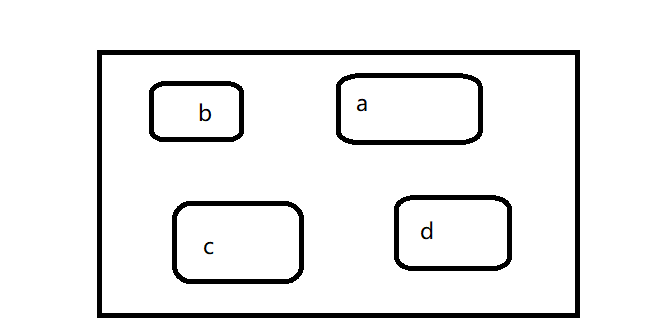
\includegraphics{img/ch7-1} \end{center}

每个名字都指向存储在内存中的一个对象

\begin{Shaded}
\begin{Highlighting}[]
\NormalTok{e <-}\StringTok{ }\KeywordTok{new.env}\NormalTok{()}
\NormalTok{e}\OperatorTok{$}\NormalTok{a <-}\StringTok{ }\OtherTok{FALSE}
\NormalTok{e}\OperatorTok{$}\NormalTok{b <-}\StringTok{ "a"}
\NormalTok{e}\OperatorTok{$}\NormalTok{c <-}\StringTok{ }\FloatTok{2.3}
\NormalTok{e}\OperatorTok{$}\NormalTok{d <-}\StringTok{ }\DecValTok{1}\OperatorTok{:}\DecValTok{3}
\end{Highlighting}
\end{Shaded}

\begin{center}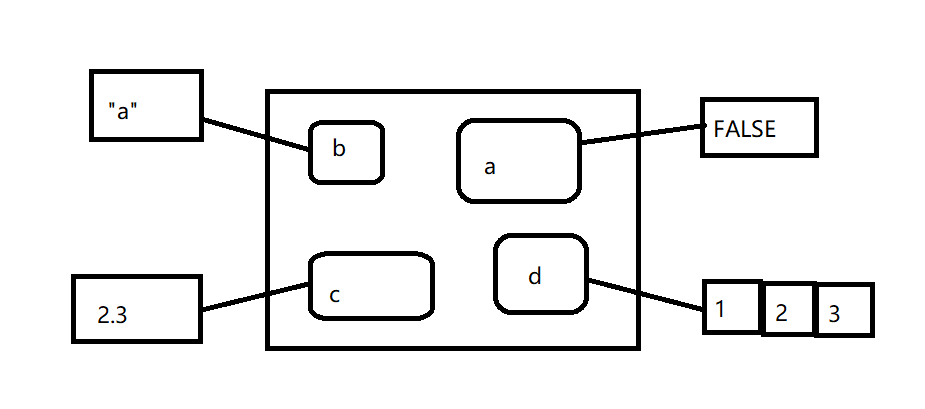
\includegraphics{img/ch7-2} \end{center}

对象并不生存在环境中,所以多个名字可指向同一个对象

\begin{Shaded}
\begin{Highlighting}[]
\NormalTok{e}\OperatorTok{$}\NormalTok{a <-}\StringTok{ }\NormalTok{e}\OperatorTok{$}\NormalTok{d}
\end{Highlighting}
\end{Shaded}

\begin{center}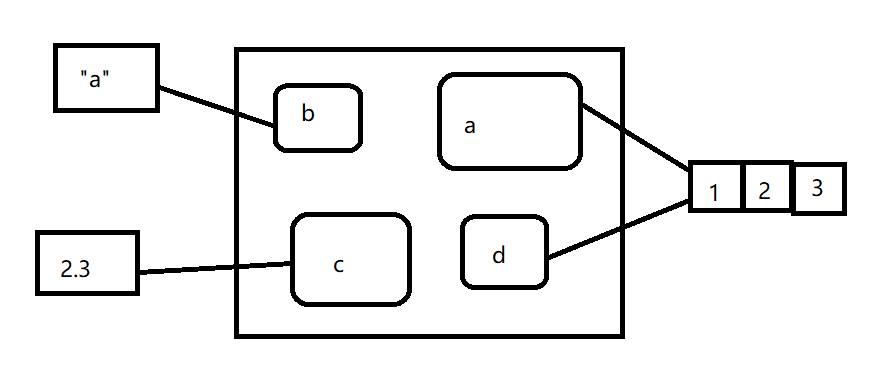
\includegraphics{img/ch7-3} \end{center}

令人困惑的是,他们还可以指向具有相同值得不同对象

\begin{Shaded}
\begin{Highlighting}[]
\NormalTok{e}\OperatorTok{$}\NormalTok{a <-}\StringTok{ }\DecValTok{1}\OperatorTok{:}\DecValTok{3}
\end{Highlighting}
\end{Shaded}

\begin{center}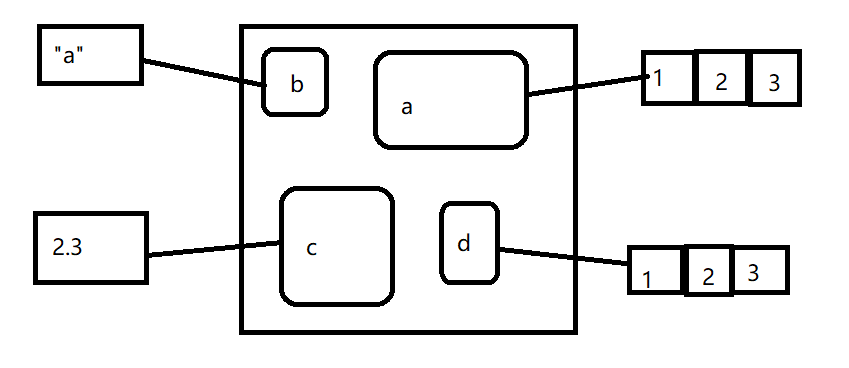
\includegraphics{img/ch7-4} \end{center}

如果对象没有指向它的名字,那么这个对象就会被垃圾回收器自动删除。

每个环境都有父环境,他是另外一个环境。在下图中,黑色小圆球代表指向父环境的指针,父环境用于实现词法作用域:如果一个名字在一个环境中没有找到,R就会到他的父环境去找(直到找到或遍历所有环境),只有空(empty)环境没有父环境

\begin{center}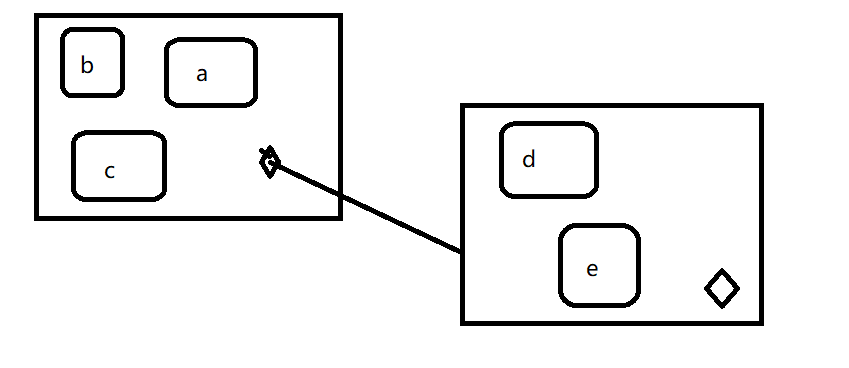
\includegraphics{img/ch7-5} \end{center}

我们可以将环境之间的关系比作家庭中成员的关系。一个环境的爷爷就是他父亲的父亲,它的祖先就包括直到空环境的所有父环境。我们基本上不会说一个环境的子环境,因为他们之间没有反向链接,给定一个环境我们没有办法找到它的子环境。

通常环境与列表相似,除一下4点外:

\begin{itemize}
\item
  环境中的每个对象都有唯一的名字
\item
  环境中的对象没有顺序
\item
  环境有父环境
\item
  环境具有引用语义
\end{itemize}

更专业一点,环境是有两部分构成:对象框,它包含名称-对象的绑定关系(行为商更像一个命名列表);它的父环境。

还有4个特殊的环境:

\begin{itemize}
\item
  globaenv()或者全局环境,他是一个交互式的工作环境,通常情况下我们就是在这个环境工作。全局环境的父环境就是libtary()或require()添加的最后一个包
\item
  baseenv(),基础环境,他是R基础软件包的环境,他的父环境是空环境
\item
  emptyenv(),空环境,他是所有环境的祖先,也是唯一一个没有父环境的环境
\item
  environment(),他是当前环境
\end{itemize}

下面看一些环境方面的方法:

\begin{itemize}
\tightlist
\item
  search()
\end{itemize}

列出全局环境的所有父环境

\begin{Shaded}
\begin{Highlighting}[]
\KeywordTok{search}\NormalTok{()}
\end{Highlighting}
\end{Shaded}

\begin{verbatim}
##  [1] ".GlobalEnv"        "package:R6"        "package:pryr"     
##  [4] "package:stats"     "package:graphics"  "package:grDevices"
##  [7] "package:utils"     "package:datasets"  "package:methods"  
## [10] "Autoloads"         "package:base"
\end{verbatim}

\begin{itemize}
\tightlist
\item
  as.environment()
\end{itemize}

访问搜索列表中的任何环境

\begin{Shaded}
\begin{Highlighting}[]
\KeywordTok{as.environment}\NormalTok{(}\StringTok{"package:stats"}\NormalTok{)}
\end{Highlighting}
\end{Shaded}

\begin{verbatim}
## <environment: package:stats>
## attr(,"name")
## [1] "package:stats"
## attr(,"path")
## [1] "D:/R-3.4.3/library/stats"
\end{verbatim}

\begin{itemize}
\tightlist
\item
  new.env()
\end{itemize}

手动创建一个环境,ls()可以列出将此环境的对象框中的所有绑定关系列出来,可以使用parent.env()查看他的父环境。

\begin{Shaded}
\begin{Highlighting}[]
\NormalTok{e <-}\StringTok{ }\KeywordTok{new.env}\NormalTok{()}

\KeywordTok{parent.env}\NormalTok{(e)}
\end{Highlighting}
\end{Shaded}

\begin{verbatim}
## <environment: R_GlobalEnv>
\end{verbatim}

\begin{Shaded}
\begin{Highlighting}[]
\KeywordTok{ls}\NormalTok{(e)}
\end{Highlighting}
\end{Shaded}

\begin{verbatim}
## character(0)
\end{verbatim}

对一个环境中的绑定关系进行修改的最简单的方法就是将其看做列表

\begin{Shaded}
\begin{Highlighting}[]
\NormalTok{e}\OperatorTok{$}\NormalTok{a <-}\StringTok{ }\DecValTok{1}
\NormalTok{e}\OperatorTok{$}\NormalTok{b <-}\StringTok{ }\DecValTok{2}
\KeywordTok{ls}\NormalTok{(e)}
\end{Highlighting}
\end{Shaded}

\begin{verbatim}
## [1] "a" "b"
\end{verbatim}

\begin{Shaded}
\begin{Highlighting}[]
\NormalTok{e}\OperatorTok{$}\NormalTok{a}
\end{Highlighting}
\end{Shaded}

\begin{verbatim}
## [1] 1
\end{verbatim}

默认情况下,ls()只能列出不是一``.''开始的名字,可以通过设置参数all.names=TRUE来显示一个环境中的所有绑定关系:

\begin{Shaded}
\begin{Highlighting}[]
\NormalTok{e}\OperatorTok{$}\NormalTok{.a <-}\StringTok{ }\DecValTok{2}
\KeywordTok{ls}\NormalTok{(e)}
\end{Highlighting}
\end{Shaded}

\begin{verbatim}
## [1] "a" "b"
\end{verbatim}

\begin{Shaded}
\begin{Highlighting}[]
\KeywordTok{ls}\NormalTok{(e,}\DataTypeTok{all.names=}\OtherTok{TRUE}\NormalTok{)}
\end{Highlighting}
\end{Shaded}

\begin{verbatim}
## [1] ".a" "a"  "b"
\end{verbatim}

\begin{itemize}
\tightlist
\item
  ls.str()
\end{itemize}

它可以将环境中的所有对象都显示出来,比str()更有用

\begin{Shaded}
\begin{Highlighting}[]
\KeywordTok{str}\NormalTok{(e)}
\end{Highlighting}
\end{Shaded}

\begin{verbatim}
## <environment: 0x000000002126a890>
\end{verbatim}

\begin{Shaded}
\begin{Highlighting}[]
\KeywordTok{ls.str}\NormalTok{(e)}
\end{Highlighting}
\end{Shaded}

\begin{verbatim}
## a :  num 1
## b :  num 2
\end{verbatim}

\begin{itemize}
\tightlist
\item
  获取绑定值
\end{itemize}

\begin{Shaded}
\begin{Highlighting}[]
\NormalTok{e}\OperatorTok{$}\NormalTok{c <-}\StringTok{ }\DecValTok{3}
\NormalTok{e}\OperatorTok{$}\NormalTok{c}
\end{Highlighting}
\end{Shaded}

\begin{verbatim}
## [1] 3
\end{verbatim}

\begin{Shaded}
\begin{Highlighting}[]
\NormalTok{e[[}\StringTok{"c"}\NormalTok{]]}
\end{Highlighting}
\end{Shaded}

\begin{verbatim}
## [1] 3
\end{verbatim}

\begin{Shaded}
\begin{Highlighting}[]
\KeywordTok{get}\NormalTok{(}\StringTok{"c"}\NormalTok{,}\DataTypeTok{envir=}\NormalTok{e)}
\end{Highlighting}
\end{Shaded}

\begin{verbatim}
## [1] 3
\end{verbatim}

\begin{itemize}
\tightlist
\item
  从环境中删除对象
\end{itemize}

\begin{Shaded}
\begin{Highlighting}[]
\NormalTok{e <-}\StringTok{ }\KeywordTok{new.env}\NormalTok{()}
\NormalTok{e}\OperatorTok{$}\NormalTok{a <-}\StringTok{ }\DecValTok{1}
\NormalTok{e}\OperatorTok{$}\NormalTok{a <-}\StringTok{ }\OtherTok{NULL} \CommentTok{#这样相当于创建了一个新的对象}
\KeywordTok{ls}\NormalTok{(e)}
\end{Highlighting}
\end{Shaded}

\begin{verbatim}
## [1] "a"
\end{verbatim}

\begin{Shaded}
\begin{Highlighting}[]
\KeywordTok{rm}\NormalTok{(}\StringTok{"a"}\NormalTok{,}\DataTypeTok{envir=}\NormalTok{e)}
\KeywordTok{ls}\NormalTok{(e)}
\end{Highlighting}
\end{Shaded}

\begin{verbatim}
## character(0)
\end{verbatim}

\begin{itemize}
\tightlist
\item
  exists()
\end{itemize}

确定一个绑定是否存在

\begin{Shaded}
\begin{Highlighting}[]
\NormalTok{x <-}\StringTok{ }\DecValTok{10}
\KeywordTok{exists}\NormalTok{(}\StringTok{"x"}\NormalTok{,}\DataTypeTok{envir=}\NormalTok{e) }\CommentTok{#查找父环境}
\end{Highlighting}
\end{Shaded}

\begin{verbatim}
## [1] TRUE
\end{verbatim}

\begin{Shaded}
\begin{Highlighting}[]
\KeywordTok{exists}\NormalTok{(}\StringTok{"x"}\NormalTok{,}\DataTypeTok{envir=}\NormalTok{e,}\DataTypeTok{inherits=}\OtherTok{FALSE}\NormalTok{) }\CommentTok{#不希望在父环境中查找}
\end{Highlighting}
\end{Shaded}

\begin{verbatim}
## [1] FALSE
\end{verbatim}

\begin{itemize}
\tightlist
\item
  identical()
\end{itemize}

identical()与==是不同的,是对两个环境进行比较

\begin{Shaded}
\begin{Highlighting}[]
\KeywordTok{identical}\NormalTok{(}\KeywordTok{globalenv}\NormalTok{(),}\KeywordTok{environment}\NormalTok{())}
\end{Highlighting}
\end{Shaded}

\begin{verbatim}
## [1] TRUE
\end{verbatim}

\begin{Shaded}
\begin{Highlighting}[]
\CommentTok{#globalenv()==environment()}
\end{Highlighting}
\end{Shaded}

\section{环境递归}

环境可以构成一棵树,因此我们非常方便的写出一个递归函数,pryr::where()会使用R的作用域法则找到定义这个名字的空间

\begin{Shaded}
\begin{Highlighting}[]
\KeywordTok{library}\NormalTok{(pryr)}
\NormalTok{x <-}\StringTok{ }\DecValTok{5}
\CommentTok{# where函数由两个参数,一个是查找的名字(字符串),一个是开始查找的环境}
\KeywordTok{where}\NormalTok{(}\StringTok{"x"}\NormalTok{)}
\end{Highlighting}
\end{Shaded}

\begin{verbatim}
## <environment: R_GlobalEnv>
\end{verbatim}

\begin{Shaded}
\begin{Highlighting}[]
\NormalTok{where <-}\StringTok{ }\ControlFlowTok{function}\NormalTok{(name,}\DataTypeTok{env=}\KeywordTok{parent.frame}\NormalTok{())\{}
\ControlFlowTok{if}\NormalTok{(}\KeywordTok{identical}\NormalTok{(env,}\KeywordTok{emptyenv}\NormalTok{()))\{}
  \CommentTok{# Base case}
  \KeywordTok{stop}\NormalTok{(}\StringTok{"Can't find"}\NormalTok{,name,}\DataTypeTok{call.=}\OtherTok{FALSE}\NormalTok{)}
\NormalTok{\}}\ControlFlowTok{else} \ControlFlowTok{if}\NormalTok{(}\KeywordTok{exists}\NormalTok{(name,}\DataTypeTok{envir=}\NormalTok{env,}\DataTypeTok{inherits=}\OtherTok{FALSE}\NormalTok{))\{}
  \CommentTok{#Success case}
\NormalTok{  env}
\NormalTok{\}}\ControlFlowTok{else}\NormalTok{\{}
  \CommentTok{#Recursive case}
  \KeywordTok{where}\NormalTok{(name,}\KeywordTok{parent.env}\NormalTok{(env))}
\NormalTok{\}}
\NormalTok{\}}
\end{Highlighting}
\end{Shaded}

有三种情况:

\begin{itemize}
\item
  基本情况: 已经到达空环境,但没有找到绑定,抛出一个错误
\item
  成功情况: 在这个环境中存在该对象,返回该环境
\item
  递归情况:在这个环境中没有找到该环境的对象,所以尝试在父环境中继续查找
\end{itemize}

\section{函数环境}

大对数环境并不是通过new.env()函数创建的,而是使用函数的结果,本节将讨论4种和函数相关的环境:封闭,绑定,执行和调用。

\begin{itemize}
\item
  封闭环境: 创建函数的环境,每个函数有且仅有一个封闭环境
\item
  使用\textless{}-讲一个函数和一个名字进行绑定,就可以定义一个绑定环境
\item
  调用函数创建一个临时的执行环境,用来存储执行期间创建的各种变量
\item
  每个执行环境都与一个调用环境关联,他说明函数在哪调用
\end{itemize}

\subsection{封闭环境}

当创建一个函数,他就获得对创建他的函数的引用,这就是封闭环境,他用作此法作用域。为了确定一个函数的封闭空间,只需调用environment()并将函数名作为第一个参数

\begin{Shaded}
\begin{Highlighting}[]
\NormalTok{y <-}\StringTok{ }\DecValTok{1}
\NormalTok{f <-}\StringTok{ }\ControlFlowTok{function}\NormalTok{(x) x}\OperatorTok{+}\NormalTok{y}

\KeywordTok{environment}\NormalTok{(f)}
\end{Highlighting}
\end{Shaded}

\begin{verbatim}
## <environment: R_GlobalEnv>
\end{verbatim}

下图中,圆角矩形代表函数,黑色菱形代表一个函数的封闭环境

\begin{center}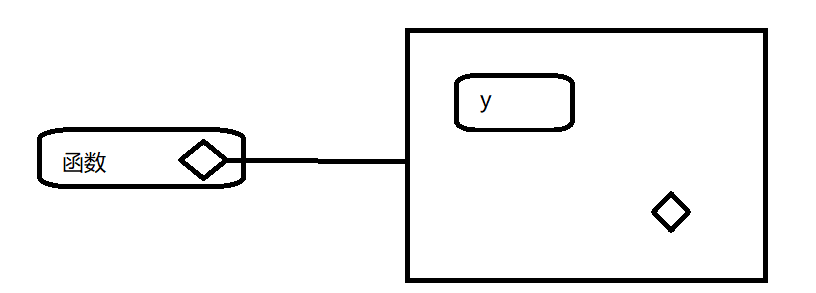
\includegraphics{img/ch7-6} \end{center}

\subsection{绑定环境}

上图太简单,因为函数没有名字,函数的名字可以通过绑定来定义,一个函数的绑定环境就是与其绑定的所有环境,下图更好的反映这种关系,因为封闭环境包含一个从f到环境的绑定

\begin{center}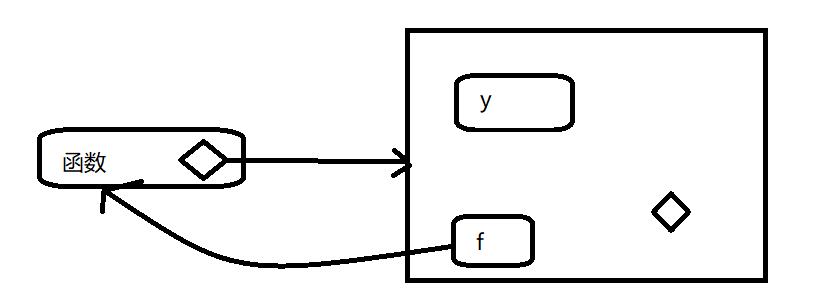
\includegraphics{img/ch7-7} \end{center}

这种情况封闭环境和绑定环境是相同的,当将一个函数分配给另一个不同的环境,那么他们就同了

\begin{Shaded}
\begin{Highlighting}[]
\NormalTok{e <-}\StringTok{ }\KeywordTok{new.env}\NormalTok{()}
\NormalTok{e}\OperatorTok{$}\NormalTok{g <-}\StringTok{ }\ControlFlowTok{function}\NormalTok{() }\DecValTok{1}
\end{Highlighting}
\end{Shaded}

\begin{center}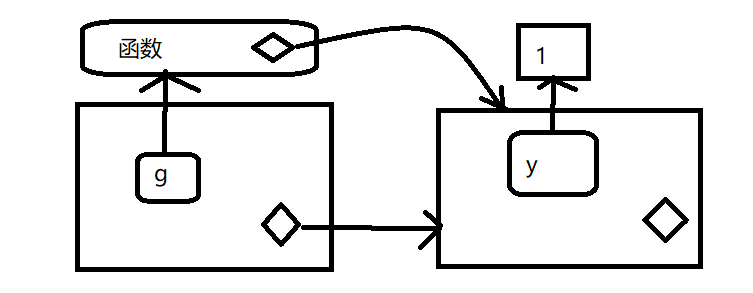
\includegraphics{img/ch7-8} \end{center}

封闭函数属于该环境,永远也不会发生改变,甚至将该函数移动到其他环境中,封闭环境决定了这个函数该如何找到值,而绑定环境空间决定如何找到该函数。

绑定空间与封闭空间的区别在于软件包命名空间是非常重要的,例如如果软件包中A使用基础包中的mean()函数,那么如果软件包B也创建了自己的mean()函数会有什么后果呢?命名空间确保软件包A使用基础包中的mean(),而不受软件包B的影响(除非显式的调用)

命名空间使用环境来实现,利用函数不一定存在于他们的封闭环境中的事实,例如基础包中的sd()函数,它的封闭环境与绑定环境是不同的

\begin{Shaded}
\begin{Highlighting}[]
\KeywordTok{environment}\NormalTok{(sd)}
\end{Highlighting}
\end{Shaded}

\begin{verbatim}
## <environment: namespace:stats>
\end{verbatim}

\begin{Shaded}
\begin{Highlighting}[]
\KeywordTok{where}\NormalTok{(}\StringTok{"sd"}\NormalTok{)}
\end{Highlighting}
\end{Shaded}

\begin{verbatim}
## <environment: package:stats>
## attr(,"name")
## [1] "package:stats"
## attr(,"path")
## [1] "D:/R-3.4.3/library/stats"
\end{verbatim}

函数sd()的定义使用var(),但是如果创建自己的var()函数,那么他也不会影响sd()

\begin{Shaded}
\begin{Highlighting}[]
\NormalTok{x <-}\StringTok{ }\DecValTok{1}\OperatorTok{:}\DecValTok{10}
\KeywordTok{sd}\NormalTok{(x)}
\end{Highlighting}
\end{Shaded}

\begin{verbatim}
## [1] 3.02765
\end{verbatim}

\begin{Shaded}
\begin{Highlighting}[]
\NormalTok{var <-}\StringTok{ }\ControlFlowTok{function}\NormalTok{(x,}\DataTypeTok{na.rm=}\OtherTok{TRUE}\NormalTok{) }\DecValTok{100}

\KeywordTok{sd}\NormalTok{(x)}
\end{Highlighting}
\end{Shaded}

\begin{verbatim}
## [1] 3.02765
\end{verbatim}

这是可执行的,因为每个软件包有两个与他相关的环境:软件包环境和命名空间环境。软件包环境包含所有可以访问的公共函数,并且存放在搜索路径上,命名空间环境包含所有函数,并且它的父环境也是比较重要的环境,其中包含了这个软件包需要的所有函数的绑定。软件包中的每一个到处函数都绑定到软件包环境,但都在命名空间环境中,如下图展示杉树关系:

\begin{center}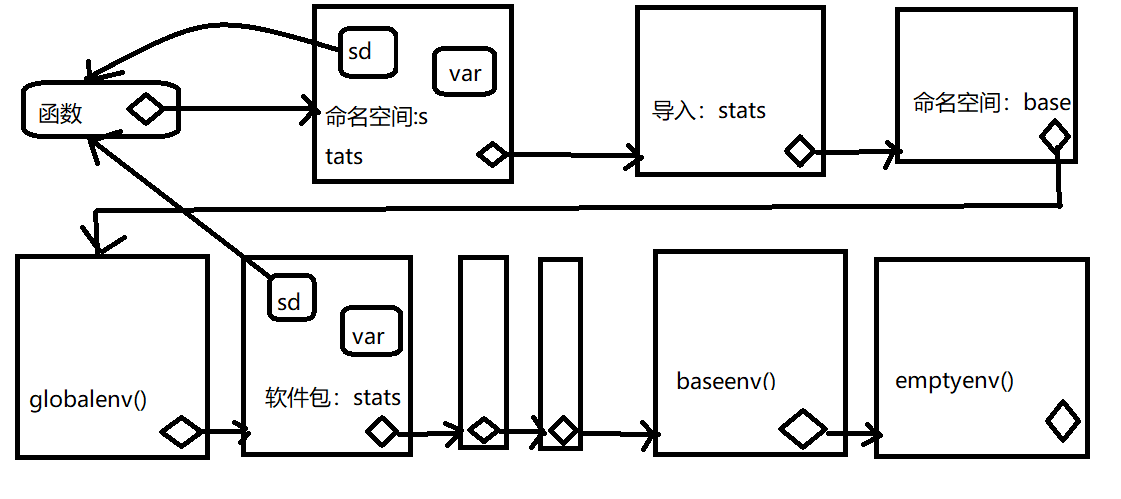
\includegraphics{img/ch7-9} \end{center}

当输入var时,R首先会到全局环境中进行查找,当sd()查找var()时,他首先到命名空间中查找,而永远不会到globalenv()中查找。

\subsection{执行环境}

第一次执行下面的函数他返回什么?,第二次呢?

\begin{Shaded}
\begin{Highlighting}[]
\NormalTok{g <-}\StringTok{ }\ControlFlowTok{function}\NormalTok{(x) \{}
  \ControlFlowTok{if}\NormalTok{(}\OperatorTok{!}\KeywordTok{exists}\NormalTok{(}\StringTok{"a"}\NormalTok{,}\DataTypeTok{inherits=}\OtherTok{FALSE}\NormalTok{))\{}
    \KeywordTok{message}\NormalTok{(}\StringTok{"Default a"}\NormalTok{)}
\NormalTok{    a <-}\StringTok{ }\DecValTok{1}
\NormalTok{  \} }\ControlFlowTok{else}\NormalTok{ \{}
\NormalTok{    a <-}\StringTok{ }\NormalTok{a }\OperatorTok{+}\StringTok{ }\DecValTok{1}
\NormalTok{  \}}
\NormalTok{  a}
\NormalTok{\}}

\KeywordTok{g}\NormalTok{(}\DecValTok{10}\NormalTok{)}
\end{Highlighting}
\end{Shaded}

\begin{verbatim}
## Default a
\end{verbatim}

\begin{verbatim}
## [1] 1
\end{verbatim}

\begin{Shaded}
\begin{Highlighting}[]
\KeywordTok{g}\NormalTok{(}\DecValTok{10}\NormalTok{)}
\end{Highlighting}
\end{Shaded}

\begin{verbatim}
## Default a
\end{verbatim}

\begin{verbatim}
## [1] 1
\end{verbatim}

每次调用这个函数都返回相同的值,每次调用函数时都创建一个新的宿主执行环境,执行环境的父环境就是函数的封闭环境,一旦函数执行结束,这个环境就会被销毁。

通过图形简单了解这个过程:虚线包围的就是执行环境

\begin{Shaded}
\begin{Highlighting}[]
\NormalTok{h <-}\StringTok{ }\ControlFlowTok{function}\NormalTok{(x) \{}
\NormalTok{  a <-}\StringTok{ }\DecValTok{2}
\NormalTok{  x }\OperatorTok{+}\StringTok{ }\NormalTok{a}
\NormalTok{\}}

\NormalTok{y <-}\StringTok{ }\KeywordTok{h}\NormalTok{(}\DecValTok{1}\NormalTok{)}
\end{Highlighting}
\end{Shaded}

1.用 \(x=1\) 调用函数

\begin{center}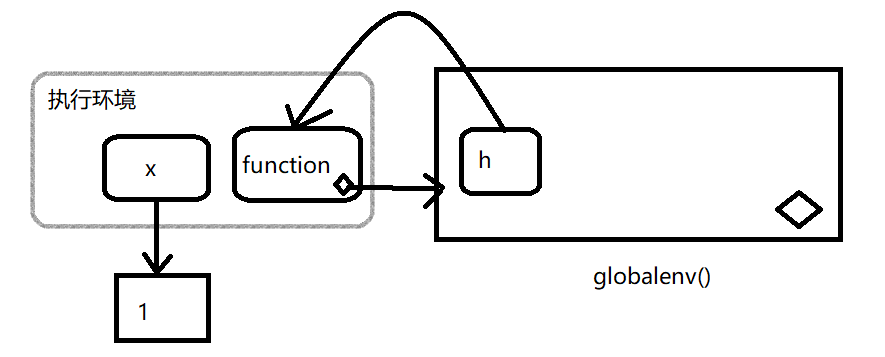
\includegraphics{img/ch7-10} \end{center}

2.a被赋值为2

\begin{center}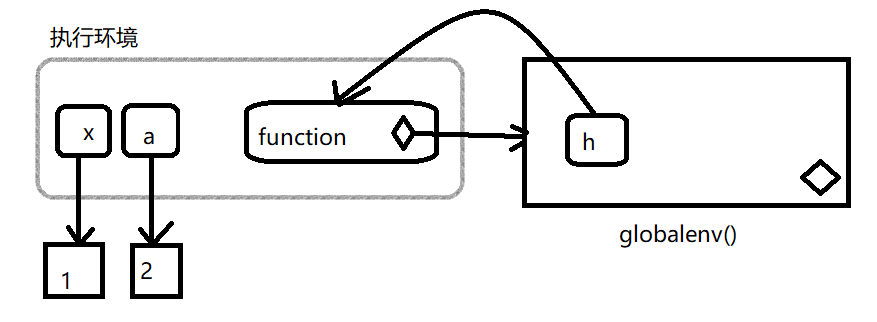
\includegraphics{img/ch7-11} \end{center}

3.函数完成后返回值为3

\begin{center}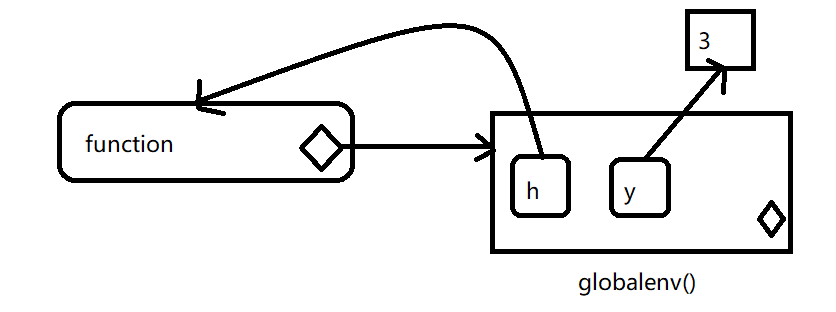
\includegraphics{img/ch7-12} \end{center}

当在另一个函数中创建一个函数的时候,子函数的封闭函数就是父函数的执行环境,而且执行环境也不再是临时的了。下面的栗子用一个函数工厂(相当于python闭包,装饰器)plus()来说明这个想法。我们使用这个工厂创建一个plus\_one()函数,plus\_one()的封闭环境是plus()的执行环境,其中x与数值1绑定

\begin{Shaded}
\begin{Highlighting}[]
\NormalTok{plus <-}\StringTok{ }\ControlFlowTok{function}\NormalTok{(x)\{}
  \ControlFlowTok{function}\NormalTok{(y) x}\OperatorTok{+}\NormalTok{y}
  \KeywordTok{message}\NormalTok{(}\StringTok{"Note: "}\NormalTok{,}\StringTok{"plus_one also a function"}\NormalTok{)}
  
\NormalTok{\}}
\NormalTok{plus_one <-}\StringTok{ }\KeywordTok{plus}\NormalTok{(}\DecValTok{1}\NormalTok{)}
\end{Highlighting}
\end{Shaded}

\begin{verbatim}
## Note: plus_one also a function
\end{verbatim}

\begin{Shaded}
\begin{Highlighting}[]
\CommentTok{#注意plus_one也是一个函数}
\end{Highlighting}
\end{Shaded}

\begin{center}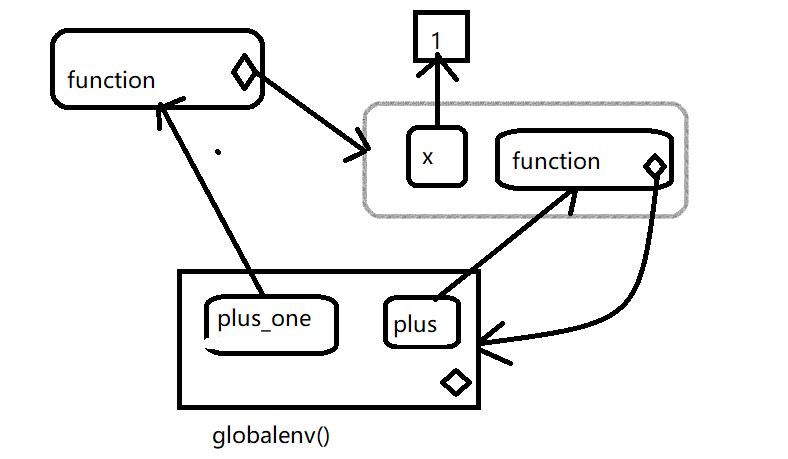
\includegraphics{img/ch7-13} \end{center}

\subsection{调用环境}

查看下面代码。当代码运行时,你期望i()返回什么?

\begin{Shaded}
\begin{Highlighting}[]
\NormalTok{h <-}\StringTok{ }\ControlFlowTok{function}\NormalTok{()\{}
\NormalTok{  x <-}\StringTok{ }\DecValTok{10}
  \ControlFlowTok{function}\NormalTok{()\{}
\NormalTok{    def <-}\StringTok{ }\KeywordTok{get}\NormalTok{(}\StringTok{"x"}\NormalTok{,}\KeywordTok{environment}\NormalTok{())}
    \CommentTok{#返回函数被调用的环境}
\NormalTok{    call <-}\StringTok{ }\KeywordTok{get}\NormalTok{(}\StringTok{"x"}\NormalTok{,}\KeywordTok{parent.frame}\NormalTok{())}
    \KeywordTok{list}\NormalTok{(}\DataTypeTok{defined=}\NormalTok{def,}\DataTypeTok{called=}\NormalTok{call,}\DataTypeTok{x=}\NormalTok{x)}
    \CommentTok{#x}
\NormalTok{  \}}
\NormalTok{\}}

\NormalTok{i <-}\StringTok{ }\KeywordTok{h}\NormalTok{()}
\NormalTok{x <-}\StringTok{ }\DecValTok{20}
\KeywordTok{i}\NormalTok{()}
\end{Highlighting}
\end{Shaded}

\begin{verbatim}
## $defined
## [1] 10
## 
## $called
## [1] 20
## 
## $x
## [1] 10
\end{verbatim}

\begin{Shaded}
\begin{Highlighting}[]
\CommentTok{#[1] 10}
\end{Highlighting}
\end{Shaded}

最外层的x(绑定到20)是为了分散你的注意力:使用普通作用域法则,h()首先找到自己是在哪里定义的,然后再寻找与x相关联的值10,但是在调用i()的环境中与x相关的值是多少?在定义h()的环境中x为10,在调用h()的环境中x为20.

注意每个执行环境都有两个父环境:一个调用环境和一个封闭环境。R普通作用域法则只使用封闭的父环境,parent.frame()允许你访问调用父环境。在调用环境而不是封闭环境中查找变量称为动态作用域(注:很少的编程语言使用动态作用域,这是因为动态调用使我们更难理解函数式如何运行的,动态调用主要用于开发交互式数据分析的函数)

\section{绑定名字和数值}

赋值操作其实就是就是将一个名字和一个值进行绑定,它对应于作用域,这个规则决定如何找到与一个名字相关联的值。可能你已经使用过上千次的R赋值语句,赋值操作为当前环境中的名称和对象建立一种绑定关系。名字通常包括字母,数字,.和\_,但是不能以\_开头,如果不遵守这些规则,则会出错。

\begin{Shaded}
\begin{Highlighting}[]
\NormalTok{_abc <-}\StringTok{ }\DecValTok{1}
\CommentTok{#Error: unexpected input in "_"}
\end{Highlighting}
\end{Shaded}

使用?Reserved可以获取完整的保留字列表,这些通常的规则也可以被重写。在一个由任何字符构成的名称的两遍加上反引号,就可以应用该名称了。

\begin{Shaded}
\begin{Highlighting}[]
\StringTok{`}\DataTypeTok{a=b}\StringTok{`}\NormalTok{ <-}\StringTok{ }\DecValTok{3}
\StringTok{`}\DataTypeTok{:)}\StringTok{`}\NormalTok{ <-}\StringTok{ "smile"}
\KeywordTok{ls}\NormalTok{()}
\end{Highlighting}
\end{Shaded}

\begin{verbatim}
##  [1] ":)"                 "a"                  "A"                 
##  [4] "a=b"                "Animal"             "area"              
##  [7] "b"                  "B"                  "b2"                
## [10] "Book"               "C"                  "c1"                
## [13] "c2"                 "cat"                "Cat"               
## [16] "cc"                 "cc2"                "circum"            
## [19] "conan"              "connan"             "Dog"               
## [22] "Duck"               "e"                  "e1"                
## [25] "e2"                 "f"                  "f1"                
## [28] "f1.character"       "f1.numeric"         "father"            
## [31] "g"                  "genderFactor"       "getShape"          
## [34] "h"                  "i"                  "j1"                
## [37] "Java"               "m1"                 "m2"                
## [40] "manager"            "member"             "Member"            
## [43] "mother"             "n1"                 "n2"                
## [46] "np6"                "NR6"                "p1"                
## [49] "Person"             "Php"                "plus"              
## [52] "plus_one"           "pr6"                "PR6"               
## [55] "R"                  "r1"                 "rc"                
## [58] "RC"                 "s"                  "s1"                
## [61] "son"                "student"            "student.attend"    
## [64] "student.default"    "student.exam"       "student.homework"  
## [67] "teacher"            "teacher.assignment" "teacher.correcting"
## [70] "teacher.default"    "teacher.lecture"    "u1"                
## [73] "u2"                 "u3"                 "User"              
## [76] "var"                "work"               "Worker"            
## [79] "x"                  "y"
\end{verbatim}

除了使用反引号外,还可以使用单引号或双引号来创建非语法的绑定,但是不推荐这样做(在赋值箭头左边使用字符串属于历史问题,在R开始支持反引号之前就已经开始使用了)

普通的赋值箭头\textless{}-总是在当前环境中创建一个变量。强制赋值箭头\textless{}\textless{}-不会再当前环境中创建变量,但是他修改父环境中已有的变量,也可以使用assign来进行深度绑定:name
\textless{}\textless{}-
value就等价于assign(``name'',value,inherits=TRUE)

\begin{Shaded}
\begin{Highlighting}[]
\NormalTok{x <-}\StringTok{ }\DecValTok{0}
\NormalTok{f <-}\StringTok{ }\ControlFlowTok{function}\NormalTok{()\{}
\NormalTok{  x <<-}\StringTok{ }\DecValTok{1}
\NormalTok{\}}

\KeywordTok{f}\NormalTok{()}
\NormalTok{x}
\end{Highlighting}
\end{Shaded}

\begin{verbatim}
## [1] 1
\end{verbatim}

还有另外两个绑定:延时绑定和主动绑定

\begin{itemize}
\tightlist
\item
  延时绑定:不是立即把结果赋给一个表达式,它创建和存储一个约定,在需要时对约定中的表达式进行求值,用特殊的赋值运算符号\%\textless{}d-\%来创建延迟绑定,他是对delayedAssign()函数的封装,如果需要更多的控制可以使用该函数。
\end{itemize}

\begin{Shaded}
\begin{Highlighting}[]
\KeywordTok{library}\NormalTok{(pryr)}
\KeywordTok{system.time}\NormalTok{(b }\OperatorTok\StringTok{ }\NormalTok{\{}\KeywordTok{Sys.sleep}\NormalTok{(}\DecValTok{1}\NormalTok{); }\DecValTok{1}\NormalTok{\})}
\end{Highlighting}
\end{Shaded}

\begin{verbatim}
##    user  system elapsed 
##       0       0       0
\end{verbatim}

\begin{Shaded}
\begin{Highlighting}[]
\KeywordTok{system.time}\NormalTok{(b)}
\end{Highlighting}
\end{Shaded}

\begin{verbatim}
##    user  system elapsed 
##       0       0       1
\end{verbatim}

\begin{itemize}
\tightlist
\item
  主动绑定:不是绑定到常量对象,相反,每次对其进行访问时都要重新计算。\%\textless{}a-\%是对基础函数makeActiveBinding()的封装。
\end{itemize}

\begin{Shaded}
\begin{Highlighting}[]
\NormalTok{x }\OperatorTok\StringTok{ }\KeywordTok{runif}\NormalTok{(}\DecValTok{1}\NormalTok{)}
\NormalTok{x}
\end{Highlighting}
\end{Shaded}

\begin{verbatim}
## [1] 0.6131557
\end{verbatim}

\begin{Shaded}
\begin{Highlighting}[]
\NormalTok{x}
\end{Highlighting}
\end{Shaded}

\begin{verbatim}
## [1] 0.6850947
\end{verbatim}

\begin{Shaded}
\begin{Highlighting}[]
\KeywordTok{rm}\NormalTok{(x)}
\end{Highlighting}
\end{Shaded}

\section{显式环境}

除了服务于作用域之外,环境也是一种很有用的数据结构,因此他们有引用语义,与R中的大多数对象不同,当你对环境进行修改时,R不会对其进行复制,例如:

\begin{Shaded}
\begin{Highlighting}[]
\NormalTok{modify <-}\StringTok{ }\ControlFlowTok{function}\NormalTok{(x)\{}
\NormalTok{  x}\OperatorTok{$}\NormalTok{a <-}\StringTok{ }\DecValTok{2}
  \KeywordTok{invisible}\NormalTok{()}
\NormalTok{\}}
\end{Highlighting}
\end{Shaded}

如果将这个函数应用于列表,原始列表不会被改变,因为修改列表实际上是创建和修改副本

\begin{Shaded}
\begin{Highlighting}[]
\NormalTok{x_}\DecValTok{1}\NormalTok{ <-}\StringTok{ }\KeywordTok{list}\NormalTok{()}

\NormalTok{x_}\DecValTok{1}\OperatorTok{$}\NormalTok{a <-}\StringTok{ }\DecValTok{1}

\KeywordTok{modify}\NormalTok{(x_}\DecValTok{1}\NormalTok{)}
\NormalTok{x_}\DecValTok{1}\OperatorTok{$}\NormalTok{a}
\end{Highlighting}
\end{Shaded}

\begin{verbatim}
## [1] 1
\end{verbatim}

\begin{Shaded}
\begin{Highlighting}[]
\CommentTok{#[1] 1}
\end{Highlighting}
\end{Shaded}

但是如果将这个函数应用于环境,那么原始环境就会被修改

\begin{Shaded}
\begin{Highlighting}[]
\NormalTok{x_e <-}\StringTok{ }\KeywordTok{new.env}\NormalTok{()}
\NormalTok{x_e}\OperatorTok{$}\NormalTok{a <-}\StringTok{ }\DecValTok{1}
\KeywordTok{modify}\NormalTok{(x_e)}
\NormalTok{x_e}\OperatorTok{$}\NormalTok{a}
\end{Highlighting}
\end{Shaded}

\begin{verbatim}
## [1] 2
\end{verbatim}

\begin{Shaded}
\begin{Highlighting}[]
\CommentTok{#[1] 2}
\end{Highlighting}
\end{Shaded}

就像可以使用列表传递数据一样,也可以使用环境,当你创建自己的环境时,应该将父环境设置为空环境,这样确保不会从其他地方继承对象:

\begin{Shaded}
\begin{Highlighting}[]
\NormalTok{x <-}\StringTok{ }\DecValTok{1}

\NormalTok{e1 <-}\StringTok{ }\KeywordTok{new.env}\NormalTok{()}

\KeywordTok{get}\NormalTok{(}\StringTok{"x"}\NormalTok{,}\DataTypeTok{envir=}\NormalTok{e1)}
\end{Highlighting}
\end{Shaded}

\begin{verbatim}
## [1] 1
\end{verbatim}

\begin{Shaded}
\begin{Highlighting}[]
\CommentTok{# e2 <- new.env(parent=emptyenv())}
\CommentTok{# get("x",envir = e2)}

\CommentTok{#Error in get("x", envir = e2) : object 'x' not found}
\end{Highlighting}
\end{Shaded}

环境时解决下面3类常见问题的有效数据结构

\begin{itemize}
\item
  避免大数据的复制
\item
  管理一个软件包的内部状态
\item
  根据名字高效的查找与其绑定的值
\end{itemize}

\subsection{避免复制}

由于环境具有引用语义,所有绝不会无意识的创建一个副本。Biocinductor包中经常使用这种技术,因为它经常需要对非常大的基因对象进行管理。在R3.1.0版本后,这种技术已经不像以前那么重要了,因为修改列表不再是深度复制了。以前修改列表的一个元素也要复制整个列表,如果有些元素非常大,就会造成昂贵的操作。

\subsection{软件包状态}

显式环境在软件包中很有用,因为他们允许你在函数调用之间保持软件包的状态,正常情况下软件包的对象是被锁定的,所以你不能直接修改他们,但是可以这样做:

\begin{Shaded}
\begin{Highlighting}[]
\NormalTok{my_env <-}\StringTok{ }\KeywordTok{new.env}\NormalTok{(}\DataTypeTok{parent =} \KeywordTok{emptyenv}\NormalTok{())}
\NormalTok{my_env}\OperatorTok{$}\NormalTok{a <-}\StringTok{ }\DecValTok{1}

\NormalTok{get_a <-}\StringTok{ }\ControlFlowTok{function}\NormalTok{()\{}
\NormalTok{  my_env}\OperatorTok{$}\NormalTok{a}
\NormalTok{\}}

\NormalTok{set_a <-}\StringTok{ }\ControlFlowTok{function}\NormalTok{(value)\{}
\NormalTok{  old <-}\StringTok{ }\NormalTok{my_env}\OperatorTok{$}\NormalTok{a}
\NormalTok{  my_env}\OperatorTok{$}\NormalTok{a <-}\StringTok{ }\NormalTok{value}
  \KeywordTok{invisible}\NormalTok{(old) }\CommentTok{#不返回old}
\NormalTok{\}}
\end{Highlighting}
\end{Shaded}

\subsection{模拟hashmap}\label{hashmap}

hashmap是一种非常有用的数据结构,它根据名字查找对象的时间复杂度为O(1)。环境默认提供这种行为,所以可以用它来模拟hashmap。CRAN的hash包就是用这种思想开发的

\section{总结}

截止到这,我们的R语言面型对象的内容介绍完了,回顾起来,首先我们介绍了R语言编程的一些规范,告诉读者要参考一些标准的规范构建自己的编程规范并在团队中做出调整,增加自己代码的可读性和运行效率,紧接着我们分了5章系统全面的介绍了R语言的面向对象编程:S3,S4,R5,R6;最后本章我们介绍了R语言环境的相关知识,环境不仅是作用域的描述,更是一种非常好用的数据结构。

最后希望阅读本电子书的R语言用户,阅读完本书后对你有一点点的帮助。

\chapter{参考文献}\label{Reference}

{[}1{]}.高级R语言编程指南{[}M{]}. hadley Wickham 著,李洪成等 译.

{[}2{]}.\href{https://wenku.baidu.com/view/fc1b919e10a6f524cdbf857d.html}{R语言面向对象编程}

{[}3{]}.数据科学中的R语言{[}M{]}. 李舰,肖凯 著.

\bibliography{book.bib,packages.bib}


\end{document}
